%
% TU/e Style Master Thesis template for LaTeX
%
% Public version 1.0
% 2010 - 2013 Thijs Nugteren and Joos Buijs
%
% THIS IS THE MAIN FILE (i.e. compile this file, compiling the others directly won't work)
%
\documentclass[a4paper,10pt,twoside]{report}

%all the other includes etc. are done in the thesis.sty file.
\usepackage{thesis}

%
% These commands need to be defined in order to produce a correct and personalized document
%
\newcommand{\shortdoctitle}{Master's Thesis}
\newcommand{\doctitle}{Investigating frameworks for integration and orchestration---a case study on a microbrewery digital twin}
\newcommand{\docsubtitle}{Master Thesis}

\newcommand{\me}{Ander Lee \\
				 1539302}
\newcommand{\keywords}{keyword1, keyword2, keyword3}
\newcommand{\version}{Version 5.1.5}
\newcommand{\monthYear}{October 2022}

%Be sure to use all the titles for your committee members!!! (their name s show up on the very first page!)
\newcommand{\firstCommitteeMember}{dr.ir. Loek Cleophas}
\newcommand{\secondCommitteeMember}{ir. David Manrique Negrin}
\newcommand{\thirdCommitteeMember}{dr.ir. Ion Barosan}
\newcommand{\fourthCommitteeMember}{dr.ir. Jeroen Keiren}

\author{\me}

%
% PDF settings
%
\pdfstringdefDisableCommands{%
  \def\\{}%
  \def\texttt#1{<#1>}%
}
\hypersetup
{
    pdfauthor={\me},
    pdftitle={\shortdoctitle},
    pdfsubject={\doctitle},
    pdfkeywords={\keywords}
}

\begin{document}

%use this include for PDF and distribution versions
\pagenumbering{roman}
\begin{titlepage}
\begin{center}

\includegraphics[height=2cm]{figures/tue-logo-high2}\\
%\LARGE
%Eindhoven University of Technology \\
\large
Department of Mathematics and Computer Science \\
Software Engineering and Technology Cluster
\vspace*{10cm}

\setlength{\TPHorizModule}{1mm}
\setlength{\TPVertModule}{\TPHorizModule}
% Set the Paragraph Indent to zero, so the first line is not Indented
% Back-up the current value so it can be put back at the end of the title page
\newlength{\backupparindent}
\setlength{\backupparindent}{\parindent}
\setlength{\parindent}{0mm}			
% Begins a textbox at 72 mm from the left of the edge of the paper and 89 mm from the top
% The width of the textbox is 95 mm (167 - 72 mm)
% The height of the box cannot be defined, so it is your task to keep the text not too long
\begin{textblock}{95}(62,89)
    \vspace*{1mm}
    \Large
    \textbf{\doctitle \\}
    \Large
    \vspace*{5mm}
    \textit{\docsubtitle}\\
    \vspace*{10mm}
    \Large
    \me\\
\end{textblock}

\large
Supervisor:\\
\begin{tabular}{c}
    \firstCommitteeMember\\
\end{tabular}

\vspace*{2mm}

\large
Mentor:\\
\begin{tabular}{c}
    \secondCommitteeMember\\
\end{tabular}

\vspace*{2mm}

\large
Committee:\\
\begin{tabular}{c}
    \thirdCommitteeMember\\
    \fourthCommitteeMember\\
\end{tabular}

\vfill
\version

\vfill
%\docdate \\
\large
Eindhoven, \monthYear\\

% Put the Paragraph Indent back to its original value
\setlength{\parindent}{\backupparindent}
\end{center}
\end{titlepage} 
\normalsize

\clearpage

%Sometimes line numbers are nice, uncomment the next line to enable:
%\linenumbers

%It could be handy to have a list of todos and brainstorms in your thesis
%\chapter*{*General todos*}\todo{remove this chapter}
%\input{chapters/general_todos}

%\chapter*{*Brainstorm results*}\todo{remove this chapter}
%\input{chapters/brainstorm_results}

\chapter*{Abstract}\label{ch:abstract}
Digital twins (DTs) are beneficial to the management of complex product life cycles because they can offer insights from both physical and virtual worlds. In order to reach its full potential, a DT often incorporates a broad range of models and toolsets. The integration and orchestration of these components pose a challenge to the DT developer. In this project, we develop a case study of a microbrewery DT and investigate frameworks that enable integration and orchestration techniques in order to simplify the design process for the trend of growing count of models in DTs.

A DT is the composite of elements from five dimensions, namely physical entities, virtual entities, services, data, and the interconnections between them. In a closed-loop, the virtual entities collect data from the physical entities, apply the data analysis services, and eventually optimize the physical entities. 

As DTs become increasingly complex, diverse tools and heterogeneous models inevitably must be brought together in order to cover all aspects of the systems. From there, the challenges in integration and orchestration arise. In short, integration concerns the encapsulation and the interface between virtual entity models. On the other hand, orchestration addresses the problem of execution sequences.
  
This study set out to investigate frameworks that embody techniques for integration and orchestration. The purpose was to identify good practices which could be reused in DT developments. A microbrewery DT was built as a case study. For now, it supports two services, namely Production Prediction and Production Control. We selected and applied three frameworks of distinctive styles to demonstrate the services. They were TwinOps---inspired by the DevOps principle; ThingsBoard---an open source platform based on the Internet of Things (IoT) and Service-Orientated Architecture (SOA); and finally Ptolemy II---based on an actor-oriented architecture which aims at experimentation in cyber-physical systems (CPS). We consider these three frameworks for their wide variety of uses, and presumed suitability for DTs.

The results indicate that a distributed framework architecture, such as TwinOps and ThingsBoard, enables a high degree of modularity and configuration which supports integration of diverse components. The extensive configuration options also contribute to a higher automation level for orchestration, as initial setup is paid off by automated processing during operations. In contrast, in a monolithic framework like Ptolemy II, the core functionalities have been unified in a self-contained package rather than assembled from a series of deployable modules or pipeline stages. As a result, it can benefit from smaller communication overhead in integration, which suggests better system timeliness. However, the same tight coupling characteristic may also restrict the flexibility of the orchestration.

Our findings highlight possible techniques for integration and orchestration. The comparison of the frameworks should be of guidance to developers considering extending a framework that suits their DT use cases.
 


\clearpage 

%An executive summary if you want:
%\chapter*{Executive summary}\label{chapter:executive_summary}
%\input{chapters/executive_summary}

%\clearpage

\chapter*{Acknowledgement}\label{ch:acknowledgement}
My special thanks go to my mentor David Manrique Negrin for his contributions to the project. He was the main supplier of the apparatuses for the brewery as well as the chemistry models. In addition, David has offered insightful advice on the design of the experiments, and the writing of this thesis.

I also want express my gratitude to my supervisor Loek Cleophas. He has monitored my progress and patiently reminded me to focus on the big picture throughout.

Finally, I am immensely grateful for my friends and family who have been an unfailing source of encouragement and reassurance. 

\clearpage 

\tableofcontents
\clearpage 

\listoffigures
\clearpage 

\listoftables
\clearpage

% \lstlistoflistings
% \clearpage

\chapter{Introduction}\label{ch:introduction}
\setcounter{page}{0}
\pagenumbering{arabic} 
The first chapter introduces the context and the main concepts of a digital twin (DT), followed by describing the current challenges associated with integration and orchestration of models in a DT. This leads to the motivation for constructing a microbrewery case study in order to investigate frameworks for integration and orchestration.

The DT concept was first introduced by Grieves in 2002 \cite{Grieves2019}. He referred to it as a concept for Product Lifecycle Management (PLM). The concept asserts that systems are dual in nature, that is, a system has a physical side and a virtual side. The premise of the model is that the two sides are bound together via a bidirectional data link.

The association to PLM is that a DT is a dynamic system that adapts to specific stages in the product's lifecycle. The stage changes made in either space are promptly translated to the subsequent outcomes in the other space. For example, the physical product may deliver data about itself or the environment to the virtual space. On the other end, the developer could tune the design on the virtual side, resulting in calibration of the physical product. This bidirectional relationship in DTs makes a clear distinction from simulations, which are frequently confused with DTs. In short, we consider that DTs go a step further by using simulations and analyses to influence the outcomes in physical space.

After Grieves' proposal of using DTs for PLM, the early adopters were from the aerospace sectors such as NASA and US Air Force \cite{Grieves2019}. The lifecycle of an aircraft normally lasts several decades \cite{boeing}. Taking a single snapshot, an aircraft is a complex composition of multi-disciplinary outputs. For instance, the jet engine is a mechanical system; the fuel system is largely based on chemical reactions; and the communication equipment is the result of electrical and computer designs. The aerospace industry has shown the utility of DTs regarding products with a broad development scale. As time passed, many more industries quickly caught up with the trend of multi-disciplinary and long-term product lifecycle. Production factories these days use dedicated software to analyze the efficiency of operations and optimize them on-the-go \cite{Zheng2018}. Hospitals also use digital assets to aid experiments on drugs and patients \cite{Kwon2022}. As a result, the study of DT development becomes more and more important.

The number and variety of DTs continue to expand these days. In the physical space, this is attributed to advancements---alongside reduction of costs---in wireless sensor networks. In the virtual space, more sophisticated modeling methods are appearing; especially, there has been a rapid progress in big-data models and artificial intelligence models \cite{Duan2019}. Under this premise we notice a problem of how to manage all the available components together in a DT in order to support the product lifecycle. To have heterogeneous tools cooperating we need integration and orchestration. These two notions include aspects as focused as data format conversion, as well as bigger considerations like inter-model scheduling. We want to investigate what are the key characteristics for integration and orchestration. 

Identifying the integration and orchestration techniques is merely the first step to improve a DT development process. Applied separately, individual techniques can hardly reduce the complexity of the process on their own. They need to be arranged in a coherent order and be governed together by operating principles. This is why we need to experiment with different frameworks for integration and orchestration in this project. A framework, simply speaking, embodies these techniques and consolidates them into a certain workflow pattern, laying out a guideline for a developer to follow. Adopting a framework when constructing DTs also ensures good practices could be reproduced consistently, as it encourages common resource utilization, for instance, through templates or libraries. Alternatively, workflow stages could also be established in the framework as discussed in the later chapters. 

An end goal of a DT is to support services in a product lifecycle. In this project we want to search for what approaches, offered by the frameworks, have the potential to enable accomplishing this goal. We choose a microbrewery as the case study, the core services we will focus on are related to the production yield aspect of the beer. A key process of a brewery is fermentation, which typically spans two weeks. The process has various variables that could be monitored by sensors, such as the alcoholic content and the temperature. Moreover, the conditions of the process are relatively mild, i.e., low temperature, medium high pressure, which allows easy observations. The fermentation process is a well studied phenomenon, making it straightforward to construct and evaluate. Taken together, these conditions within the case study give us great flexibility to test the different frameworks. 

\section{Context}\label{sec:context}
As claimed by market analysts \cite{pwc2014, ibm}, the emerging trend of Industry 4.0 is characterized by widespread digitalization. Hence DTs are becoming more widely adopted as industry moves toward a digital transformation which sets out to improve the transfer of information across the value chain. This will allow stakeholders to share knowledge about the designs, conditions, and logistics of their products and operations through digital artifacts. By facilitating the virtual mock-up of the real product, one can overcome the temporal and spatial limitations of experimenting in the physical world, thus greatly reducing the overall cost.

The concept of DT is often discussed together with the model-driven system engineering (MDSE) paradigm \cite{Bordeleau2020}. In MDSE, a complex system is treated holistically. It is described in terms of the interaction between systems, or better known as ``system of systems" \cite{Kossiakoff2011}. The system architecture is represented as models in order to support requirements, design, analysis and verification activities throughout the lifecycle. The use of modelling exploits recurring design patterns, hence helping to drive a consistent specification without significantly increasing costs as the system depth---the total number of abstraction layers---extends. It is found in many studies that DTs which follow MDSE have the potential to bring the following benefits \cite{Boschert2016, Macchi2018, Lim2019, Ansari2020, Cai2021, Gurdur2022}:
\begin{itemize}
  \item Reduced maintenance costs during a system's lifecycle.
  \item Reduced errors and inconsistencies across multiple iterations. 
  \item Improved multi-disciplinary collaboration, i.e., engineers from different job functions are able to quickly grasp the high-level overview of the design.
\end{itemize}

\section{Domain overview}\label{sec:overview}
In this section we first discuss the DT classification. After that, we provide an overview a five-dimensional view of DT which helps us to assess the individual components and their interactions.
\subsubsection{Classification}
Although the term ``digital twin" has been mentioned in much literature, such studies seldomly share the same definition \cite{Liu2021}. In some studies the definition centers on to multi-scale simulations working together \cite{Shafto2012}. In other studies it is defined as a high fidelity digital replica of the physical asset \cite{Schluse2018}. In order to find a definition that fits our case study, and to keep the later discussions consistent, we will adopt the classification proposed by Kritzinger et al. \cite{Kritzinger2018}. According to the classification, `digital twin' can be roughly divided in three categories based on the level of data integration between the physical assets and their virtual counterpart (illustrated in Figure \ref{fig:dt}):

\begin{figure}[hbt!]
  \centering
  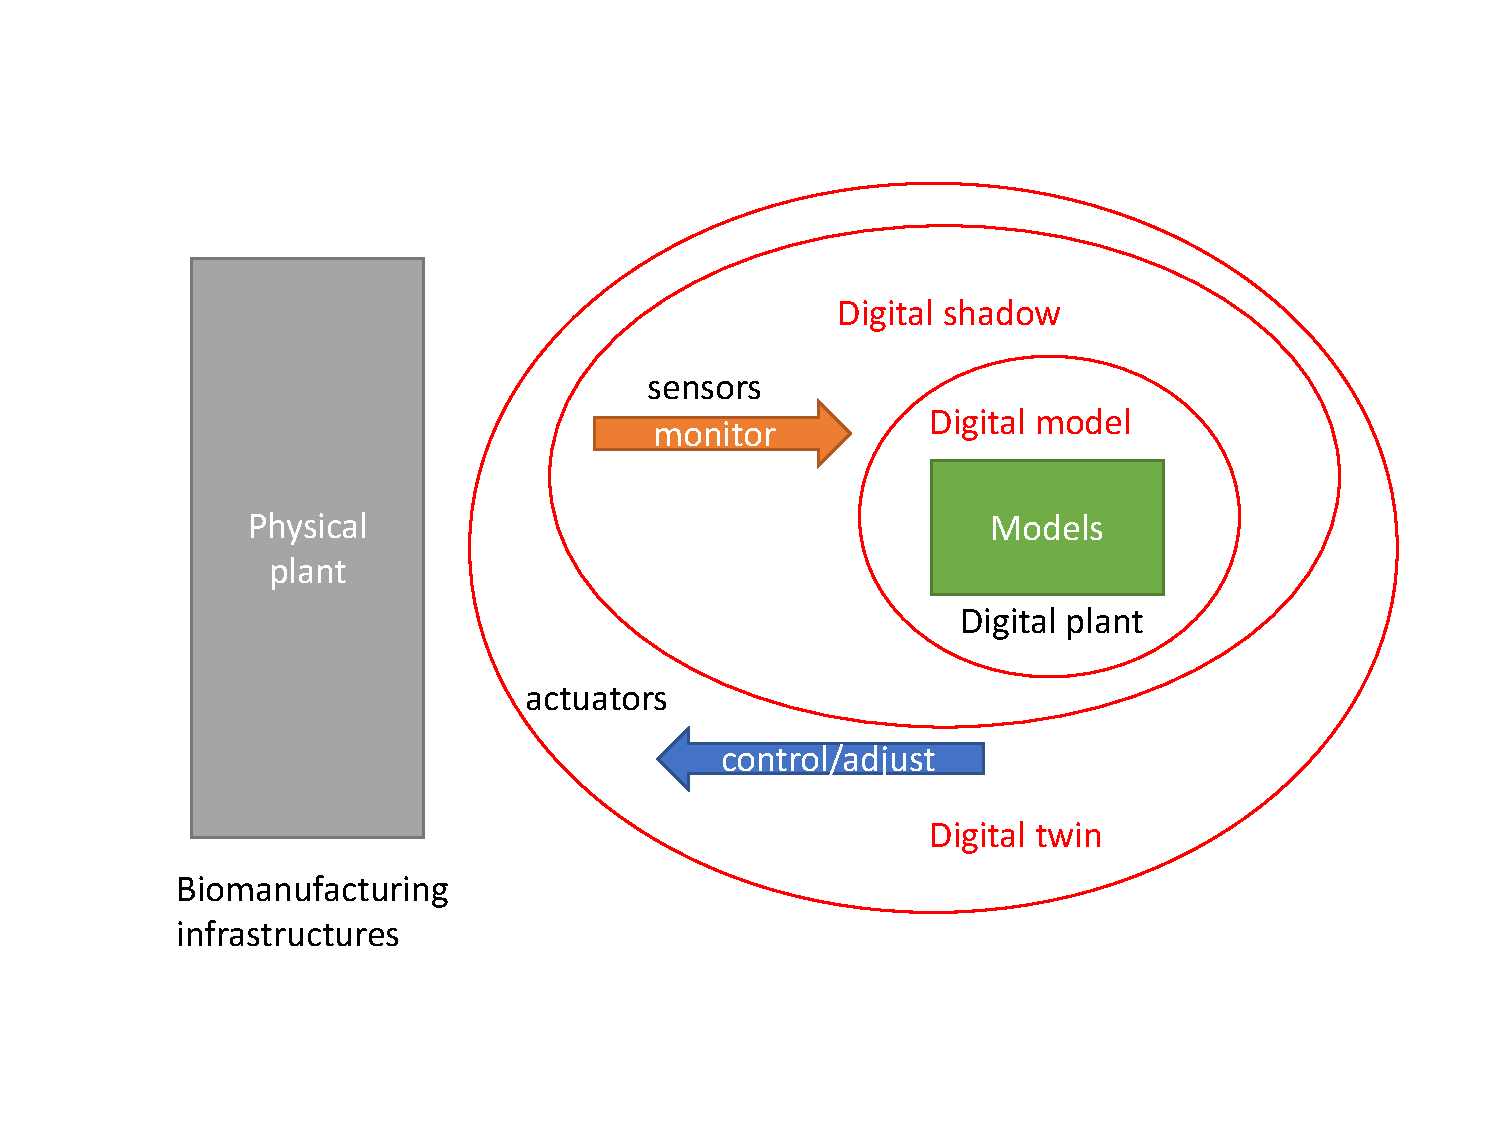
\includegraphics[scale=0.5]{figures/dt.pdf}
  \caption{Classification of digital twin}
  \label{fig:dt}
\end{figure}

\begin{itemize}

  \item \textbf{Digital model}: The virtual space does not involve data exchange with the physical space in an automated fashion. Hence the changes in one part have no direct effect on the other unless updates are performed manually.

  \item \textbf{Digital shadow}: There exists an automated one-way data communication from the physical object to the virtual one.
  
  \item \textbf{Digital twin}: Bi-directional data exchange between the physical space and the virtual space is automated. Changes made in the physical space will be reflected in the virtual space and vice versa. 

\end{itemize}

In a manufacturing plant setting, data delivered from the physical world to the virtual world is used for monitoring. The reverse direction amounts to the adjustments of actuators. It is important to note that adjusting an actuator in a DT often has a different connotation with the traditional control scheme. In an old-fashioned control style, the computed value is sent to the actuator as a direct activation of certain operations; whereas in a DT, the computed values more likely belong to the parameter set of a complex controlling model that influence the actuators in more nuances, such as adjusting the weighting factors.

A fully automated DT might be unfeasible in certain domains. In particular, for the bio-chemical domain, Udugama et al. \cite{Udugama2020, Udugama2021} recognize that human interventions are still necessary in many scenarios. In practice, it is often the case that DTs deliver the suggestions to the operator through a human machine interface (HMI) first; and the operator can act on the available data. This concept is called human-in-the-loop, and is demonstrated in \cite{Barricelli2020} for an athlete DT, where the coach manages the fitness plan for the athlete based on the reports given by the DT. Since this project concerns a microbrewery which also lies in the bio-chemical domain, the relaxed definition of DT is considered relevant.    

Another variant of DT workflow which specifically targets the bioprocessing theme is introduced in \cite{Udugama2021}. One might find the alternative relevant if the DT includes a multitude of static and dynamic chemical processes. More details can be found in Appendix \ref{apd:workflow}.

\subsubsection{Dimension}
This section introduces a DT model by Tao et al. \cite{Tao2017}, focusing on the interconnections between different parts. They propose a five-dimensional view of DT model shown in Figure \ref{fig:tao5d}. Each dimension is described as follows:

\begin{figure}[hbt!]
  \centering
  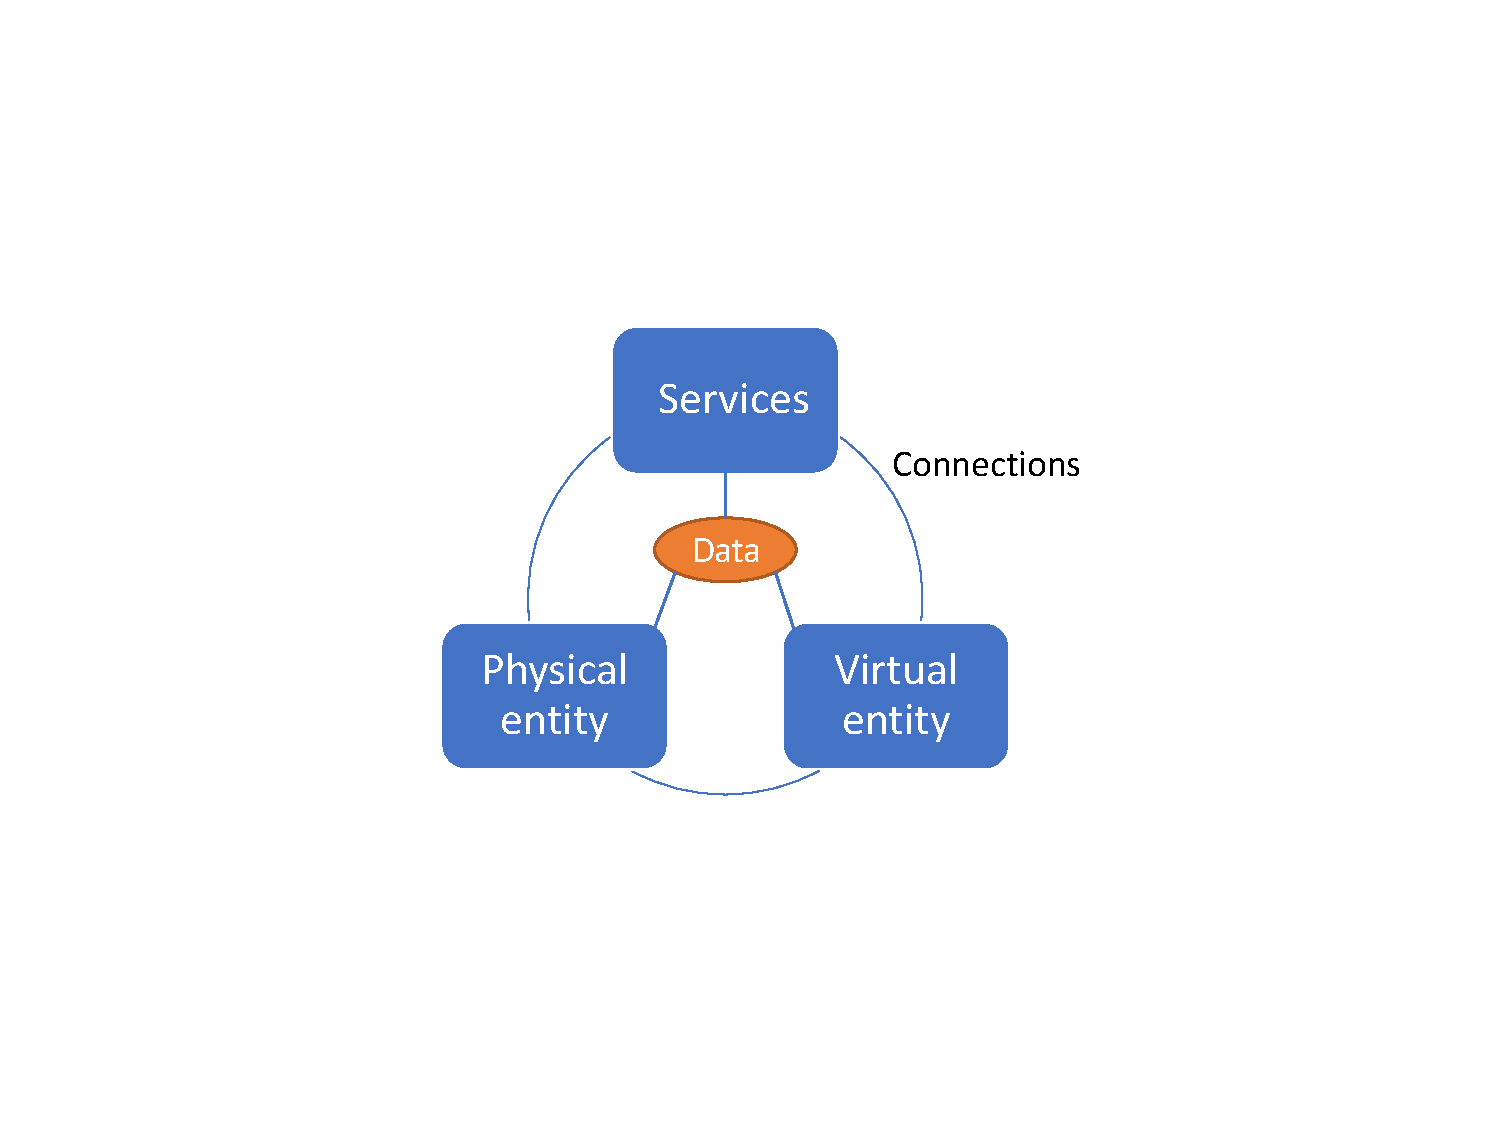
\includegraphics[scale=0.5]{figures/tao5d.pdf}
  \caption{5D view of DT model}
  \label{fig:tao5d}
\end{figure}

\begin{itemize}

  \item \textbf{Physical entity} (PE): A collection of sensors and equipment working collaboratively to collect real-time data for the intended services, meanwhile receiving control orders from the virtual world.    

  \item \textbf{Virtual entity} (VE): A digital mirror, which contains models simulating the physical counterpart with high fidelity. Calibration strategies are generated through comparing the models with entities to support models' evolution.
  
  \item \textbf{Services}: Provides various services to support the management and control of PEs as well as the operation and evolution of VEs. Services are usually requested by the users to fulfill certain functionalities.
       
  \item \textbf{Data}: A shared storage consisting of the raw data from PEs, VEs, and services. It may also be responsible for merging data from various sources to a fused format. 
   
  \item \textbf{Connections}: The connections for all four of the above-mentioned dimensions. Relevant concepts include communication protocols, access ports, etc.
  
\end{itemize}

As we can see the five elements form separate dimensions, yet it has to be ensured that they can inter-operate correctly and effectively. A main goal of integration and orchestration is to address this issue. In particular, the interoperability among VEs is what we will concentrate most on in this project, for the reason explained in the following section. 


\section{Challenges}\label{sec:challenges}
This section describes the difficulty of managing multiple models in a DT. We give explanations of why the solutions available in commercial platforms are insufficient. Hence it motivates us to look for frameworks that address the challenges. We also acknowledge that generalizing the approaches is equally important as solving for the specific microbrewery case study.

As DTs become increasingly powerful and used for complex systems, diverse tools and heterogeneous models inevitably must be used to cover all aspects for DT constructions. In this step, the challenges in integration and orchestration arise. The terms integration and orchestration can be understood as:

\begin{itemize}

  \item \textbf{Integration} couples different models by \underline{encapsulating} their properties and operations, followed by \underline{interfacing} the abstract representations with a proper communication method.

  \item \textbf{Orchestration} dictates models' \underline{execution schedule} and arranges the \underline{event queue} for the events of a particular execution.

\end{itemize}

Commercial platforms like Simulink \cite{Simulink} or CATIA \cite{CATIA} tackle the issue by expanding their ecosystem with proprietary plugins and extensions so the users can rely less on external implementations. Although these platforms still have some third-party tool support---often by means of imports---they are not promoted as common practice, and the users are more likely encouraged to use the built-in toolbox for better reliability. In the work of van den Brand et al. \cite{brand2021}, a similar observation is mentioned, stating that many commercial frameworks support integration and orchestration only to a selective modeling toolset. Therefore, we need to find a framework that extends the support to more models.

The research on an open framework that incorporates integration and orchestration as fixtures in the design workflow remains scarce. As the number of models and their interactions increases, the complexity of control and data flows will grow significantly. Adopting a framework allows the integration and orchestration to scale proportionally, and be replicated consistently. This ultimately contributes to streamlining of DT developments.

Another study produced by Negrin et al. \cite{Negrin2021} investigated the integration and orchestration concerning an autonomous truck at a distribution center. This study signifies the importance of considering the specific DT's purpose and use case context, while extracting the universal properties of integration and orchestration which can be applied in other domains.

\section{Problem definition}\label{sec:prodef}
Figure \ref{fig:intorc} illustrates the main ideas which are covered by integration and orchestration respectively. On the right side, it shows that integration comprises two aspects, namely encapsulation and interface. Encapsulation refers to the abstraction of a model, as well as discerning the relevant inputs and outputs from the rest of internal operations of the model. The common notion of a ``black box" system is a form of encapsulation. This allows the interaction with other models to take place without redundancy while still retaining all necessary information. The interface, on the other hand, is responsible for building a bridge of communication agreed by the involving models, such that the correctness---both numerical and semantic---of data can be reliably maintained. A common way of interfacing is by using an established protocol, so all data transmissions will adhere to a fixed set of rules. 

\begin{figure}[hbt!]
  \centering
  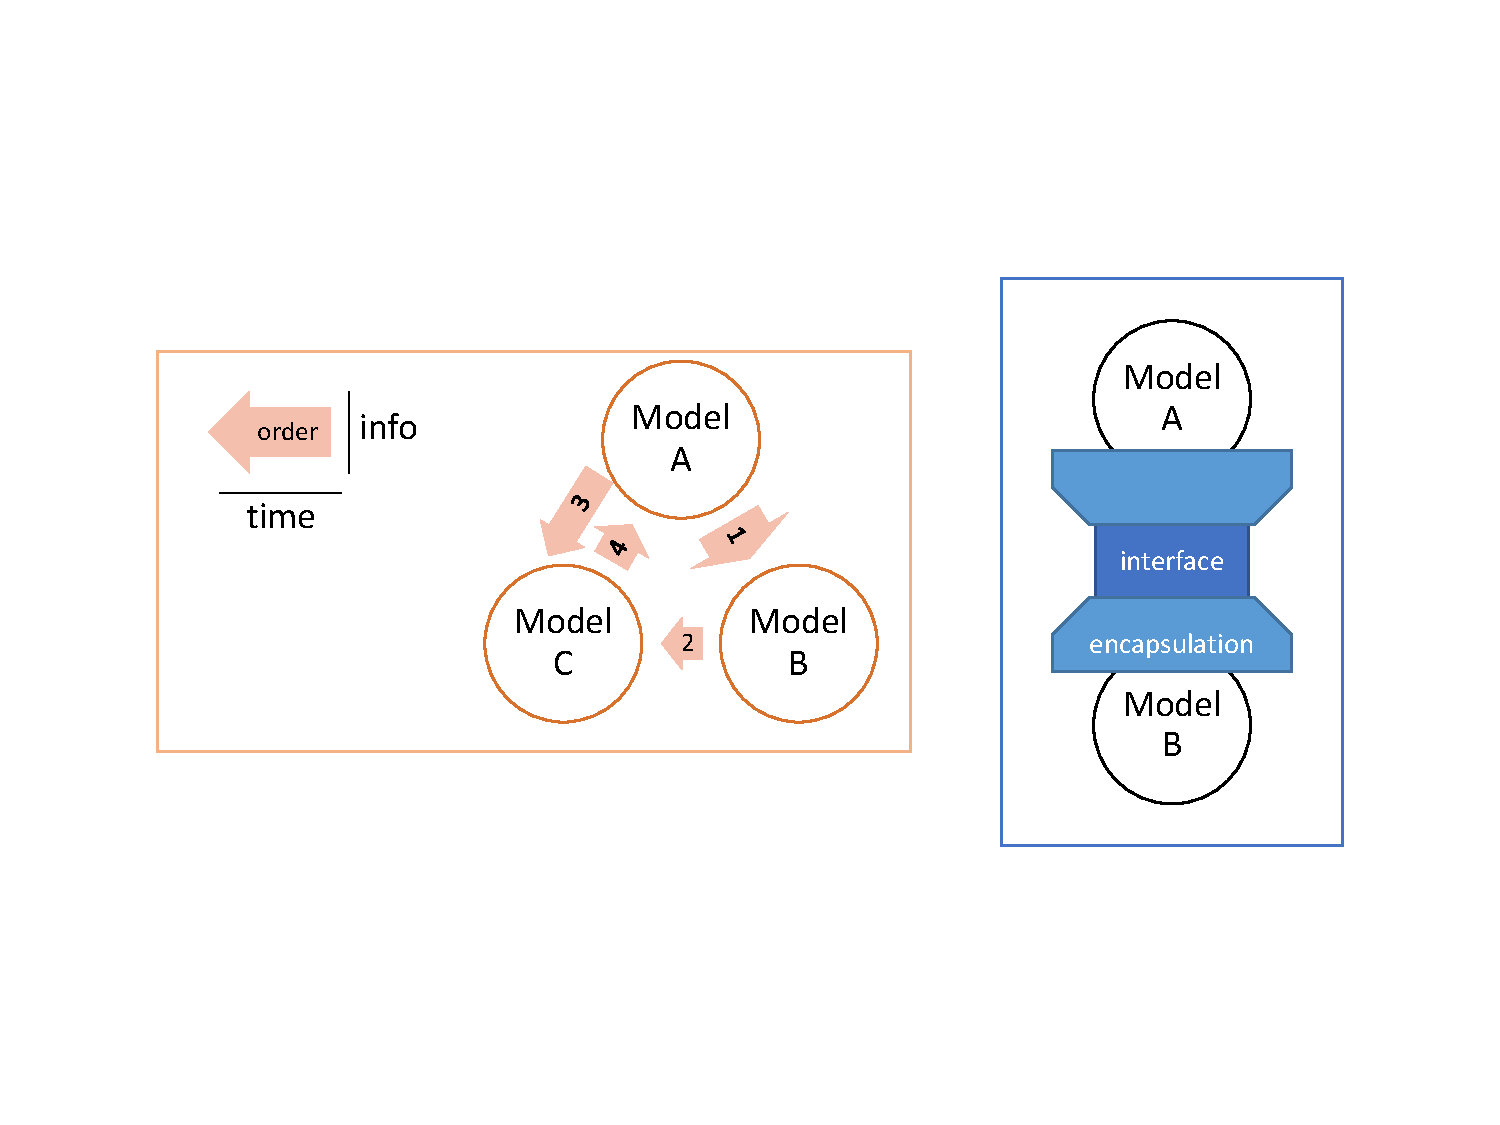
\includegraphics[scale=0.5]{figures/intorc.pdf}
  \caption{Integration (right) and orchestration (left)}
  \label{fig:intorc}
\end{figure}

On the left side, the concept of orchestration is shown. It encompasses two parts: (1) The scheduling relation between different models; in the figure it is represented by arrow shapes. The numbering in the arrows indicates the execution order. The difference in execution time incurred is represented by length variety of the arrow shapes. Furthermore, different information types may also be transferred from one model to another, whether it is a single trigger, or a stream of data, etc. The widths of the arrow shapes are used to highlight such discrepancy. (2) The handling of events, that is, the policy to control how event instances are accessed in the event queue \cite{Ptolemaeus2014}. In here the events refers to internal events of a particular execution. 

While (1) looks at individual model as an abstraction, (2) focuses on the task sequence within the model in order to ensure a deterministic outcome. A situation that might require event handling, is when several models are scheduled to execute concurrently, their respective events might arrive and leave in different order.

\section{Project Scope}\label{sec:scope}
This is an exploratory project of the possible frameworks for integration and orchestration techniques, supported by the implementation of the microbrewery DT as case study. 

The fermentation process models in the DT are given, they are developed by tutor Manrique Negrin, a hobby brewer and a chemist by training. Hence the details of these models or simulation algorithms are not within the scope. A comparative study of the three selected frameworks---detailed in Chapter \ref{ch:methodology}---will be conducted in parallel to the DT services development. Despite the considered use case being influenced by a bio-chemical theme, we strive to maintain universality in the analysis, such that the findings can be applied in other domains as well.

Functional and system level testing of the DT are also part of the implementation scope in order to evaluate the performance outcomes.

\section{Research questions}\label{sec:rqs}
Given the premises, in this study an attempt is made to answer the following research questions: 

\begin{itemize}

  \item \textbf{RQ1}: What are the key ingredients for integration and orchestration of models in different services for a microbrewery DT?
  \item \textbf{RQ2}: How can these ingredients be generalized to benefit other application domains? 
  \item \textbf{RQ3}: In what circumstances do the selected frameworks best fit these ingredients?  
  
\end{itemize}

Collectively, the answers to these research questions will lead to expanding our knowledge of: \textit{What are considered good practices for the integration and orchestration of DT models?}

\section{Report structure}
The rest of this report is structured as follows: 

\begin{itemize}

\item Chapter \ref{ch:background} presents the state of the art regarding the technologies that constitute a DT. We will also examine a number of related works which address the topic of integration and orchestration.

\item Chapter \ref{ch:methodology} describes the high-level architecture of the design process. The proposed services as well as their requirements and KPIs will be elicited. We will discuss the selected frameworks for integration and orchestration.

\item Chapter \ref{ch:implementation} describes the workflow of individual frameworks, from initial setup to resultant implementation.

\item Chapter \ref{ch:discussion} explains and compares the results between the frameworks, then summarizes the findings.

\item Chapter \ref{ch:conclusion} uses the findings to answers the research questions, and discusses future work.

\end{itemize}



\clearpage

\chapter{Background}\label{ch:background}
This chapter first covers the state of the art in DT technologies in Section \ref{sec:sota}, specifically the three major aspects of monitoring, modelling, and controlling. Although these aspects do not directly address the integration and orchestration topics, however, since they are the core parts of a DT (as explained in Section \ref{sec:overview}), the DT services will certainly rely on them to achieve the intended outcomes. We reckon it is important to be informed about the state of the art in each aspect, so that when building a DT we can take this state of the art into account---including its effects on integration and orchestration.

In Section \ref{sec:relatedwork} the discussion will shift toward the available integration and orchestration approaches, and how they have been used under the context of bioprocessing DTs.

\section{State of the art}\label{sec:sota}

We review the latest developments of monitoring, modelling, and controlling respectively. Naturally, the DT services are built upon these aspects, implying the frameworks for integration and orchestration have to accommodate them in order to ensure the services running well.

\subsection{Monitoring} \label{sec:monitoring}
In DT development, the monitoring of the physical world is normally performed using sensors. Clusters of sensing nodes may work collaboratively as enabled by Internet of Things (IoT) technologies. 

\textit{Hard sensors} normally refer to the electronic instruments that detect and collect measurements directly from their vicinity, for instance, a thermostat or pressure gauge. More advanced instruments like spectroscopies---based on the interaction of electromagnetic waves and molecular bonds to measure biomass---are gaining ground \cite{Gargalo2020}. By virtue of their computing capability of properties that are obscured or out of reach to human perceptions, these sort of advanced sensors can be placed in harsh environments such as an agitated bioreactor to provide process data while maintaining non-invasive to the system. In general, high accuracy and low latency are advisable for generating reliable online data.

\textit{Soft sensors} are the inferential sensing technology that estimate process variables that cannot be directly measured, by combining data collected from hard sensors into equations and a mathematical model. Based on the techniques, they can be categorized roughly to two classes, namely \textit{model-driven} or \textit{data-driven} \cite{Udugama2021}. \textit{Model-driven} soft sensors are built upon first principles models, which rely on in-depth knowledge of the target process, and that implies higher degree of complexity. The advantage of a model-driven approach is that it has a solid foundation based on physical laws and theories, and that allows an easier generalization of the process provided the user also possesses sufficient know-how of the field \cite{Rasheed2020}. Alternatively, \textit{data-driven} sensors are fed massive data quantities in order to generate predictions. Common approaches include black-box models such as MultiVariate Data Analysis (MVDA), a form of statistical model that processes multiple variables simultaneously and eventually aims to decrease the dimensionality. Another data-driven approach that is rapidly gaining popularity is Artificial Neural Networks (ANN), thank to the wide availability of hardware support like Graphical Processing Units (GPUs), and software library support such as TensorFlow \cite{tensorflow}, and PyTorch \cite{pytorch}.

\subsection{Modelling}
Rather similar to the classifications of soft sensors described above, modeling approaches can be sorted by their level of abstraction \cite{Narayanan2020, Zhou2021}. At the higher level, techniques like first principles and mechanistic models in biochemical domains; or Computer-Aided Design (CAD) and topological models used in mechanical domains \cite{Jiang2021} are considered knowledge-based, i.e., more demanding in domain expertise, hence requiring less online data to construct. In contrast, at a lower level of abstraction, Artificial Intelligence (AI) related techniques rely more heavily on empirical data.

The step for merging the monitored data into the model states is known as data assimilation. Recursive parameter estimation is an approach for data assimilation. It refers to taking old estimates (old model parameters) obtained from fitting one set of data points to generate new estimates when new data points (new observations) are added to the original data set \cite{Rutan1990}. Another technique within the same category is extended Kalman filter, which is broadly used to perform state estimation \cite{Oisiovici2000, Kramer2016}.

Although the models used in this project are given, it is still useful to have an understanding of what modelling techniques are used these days, because different techniques consume and generate different forms of data that may require different treatments of integration and orchestration.

\subsection{Controlling}
We can consider controlling as the last piece in DTs that ``closes the loop" between the virtual world and and the physical world. Proportional–Integral–Derivative (PID) controllers have been used  in industrial control for decades. Their popularity can be attributed the robustness and simplicity in a wide range of industrial settings \cite{pidni}. On the other hand, the advancement of high volume data acquisition enables growing adoption of model predictive control (MPC), which goes beyond merely a reactive mechanism as PID, also taking into account the contextual knowledge of the underlying complex process. Hong et al. \cite{Hong2018} examine the advantage of a hybrid scheme that combines adaptive model-based feedback with direct PID control for optimizing startup, changeover, and shutdown. The study also discusses functionally partitioning components to improve flexibility and reduce operation cost for constructing hybrid models.  

In the control service which will be introduced in Chapter \ref{ch:methodology}, we use the PID approach for its simplicity as a proof-of-concept. Nonetheless, as the microbrewery DT will continue to expand and mature, we do not rule out the possibility of migrating to the MPC approach in the future. 

\section{Related work}\label{sec:relatedwork}
This section first introduces the recent progress in integration and orchestration approaches. They serve as the references for the designs to consider when choosing the frameworks in Chapter \ref{ch:methodology}. Real case studies of DT will also be described in order to show how the integration and orchestration approaches could improve DT operations.

\subsection{Integration} \label{sec:inte}
Integration is a key step of models' communication and execution. In a production plant context, communication infrastructures commonly comprise the following aspects \cite{Gargalo2020}:

\begin{itemize}

  \item A supervisory control and data acquisition (SCADA) system that handles the interfacing of monitor and control operations. Its components include remote terminal units (RTU) for processing commands; programmable logic controllers (PLC) for processing control signals; HMI for aiding the operator in various actions.
  
  \item Data standards such as XML, JSON that deliver string-value pairs of the monitoring/controlling variables. It may also contain information about the computational pipeline of the process.
  
  \item Communication protocol stacks that address each Open Systems Interconnection (OSI) layer. Common patterns such as client/server in TCP/IP, or publish–subscribe in Message Queuing Telemetry Transport (MQTT) are well documented in IoT literature.
  
\end{itemize}

It is important that the above infrastructures are classified and understood well, because in our DT construction they will become the underlying elements supporting the services to communicate information. In Chapter \ref{ch:methodology} and \ref{ch:implementation}, some of the above notions will reoccur sporadically.

Apart from the generic infrastructures, we further introduce two open source standards that target specifically the integration in modelling, namely Computer-Aided Process Engineering (CAPE)-OPEN \cite{capeopen}, and Functional Mock-up Interface (FMI) \cite{fmi, Blochwitz2011}.

\begin{figure}[hbt!]
    \centering
    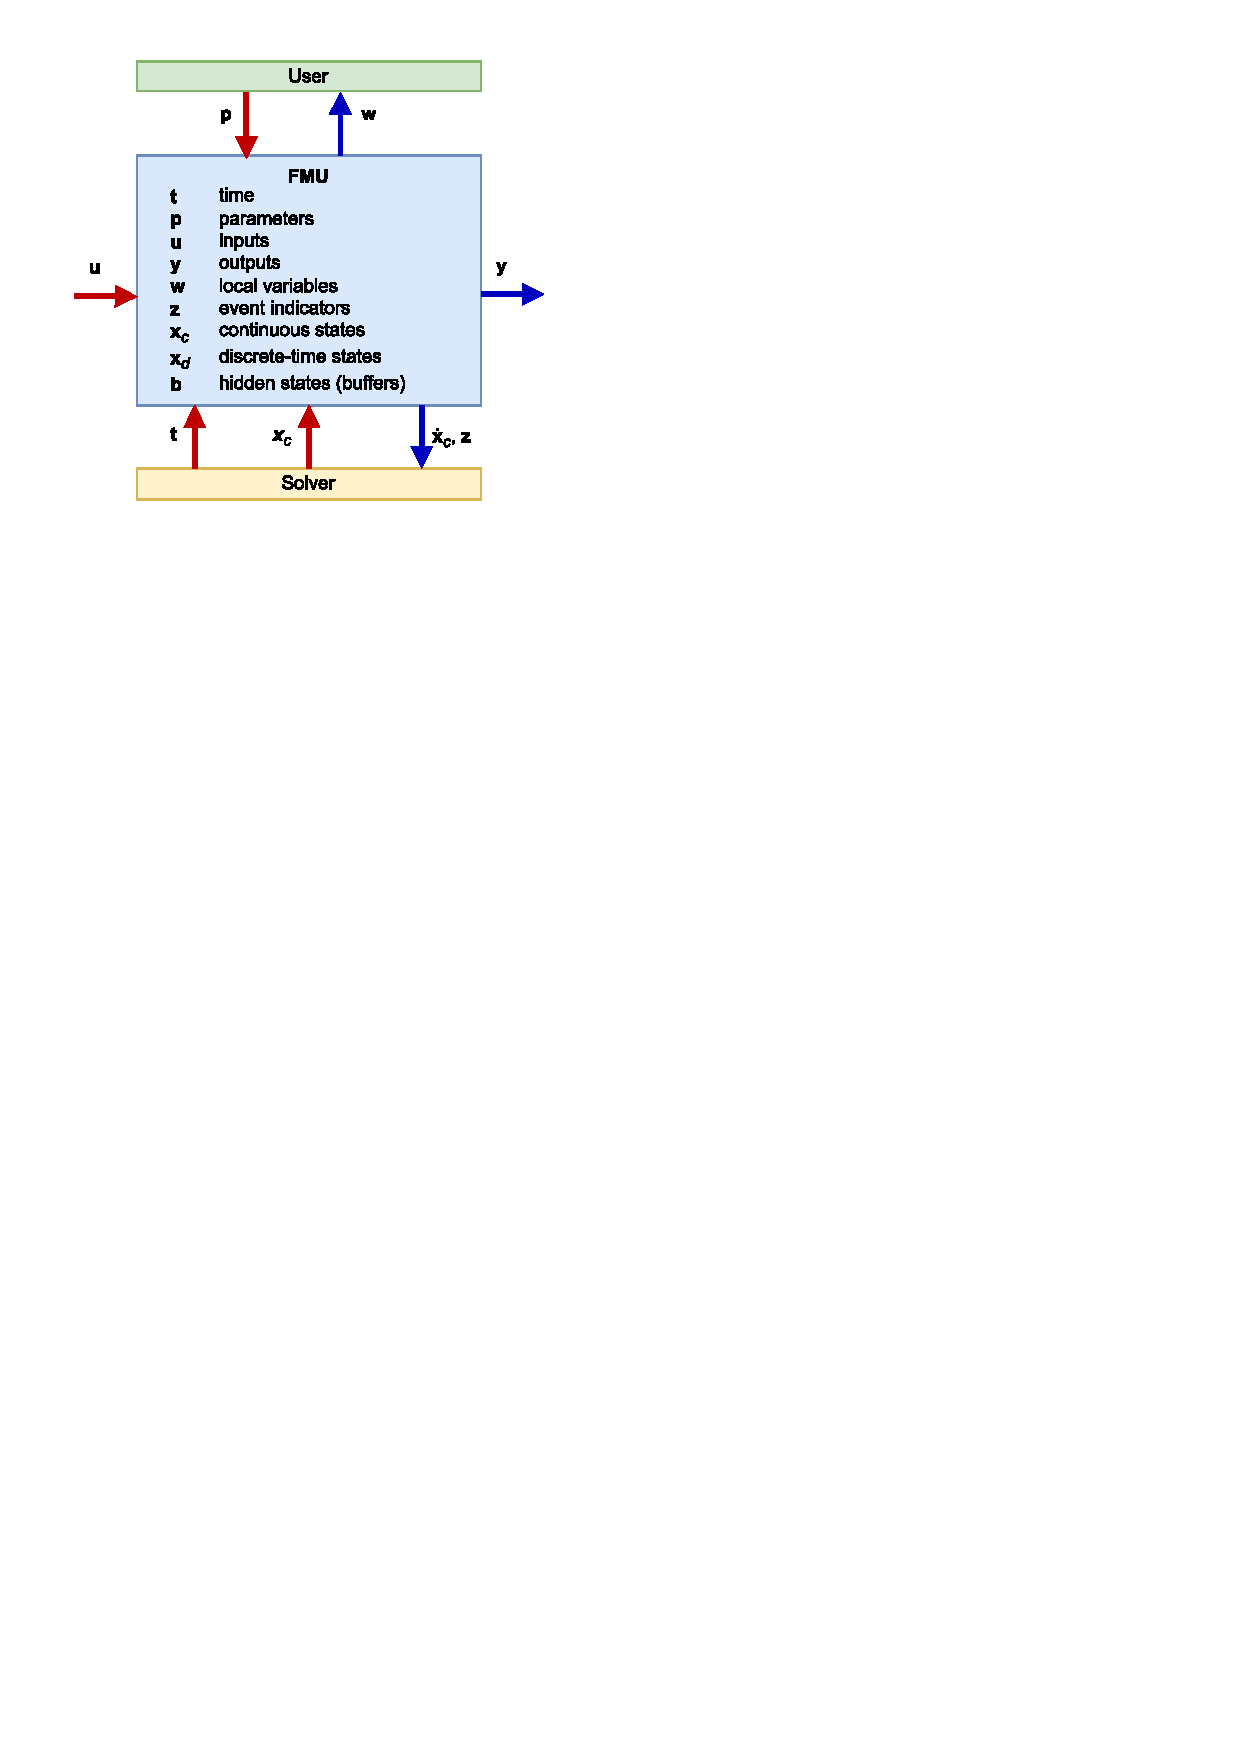
\includegraphics[scale=0.6]{figures/fmi_me.pdf}
   	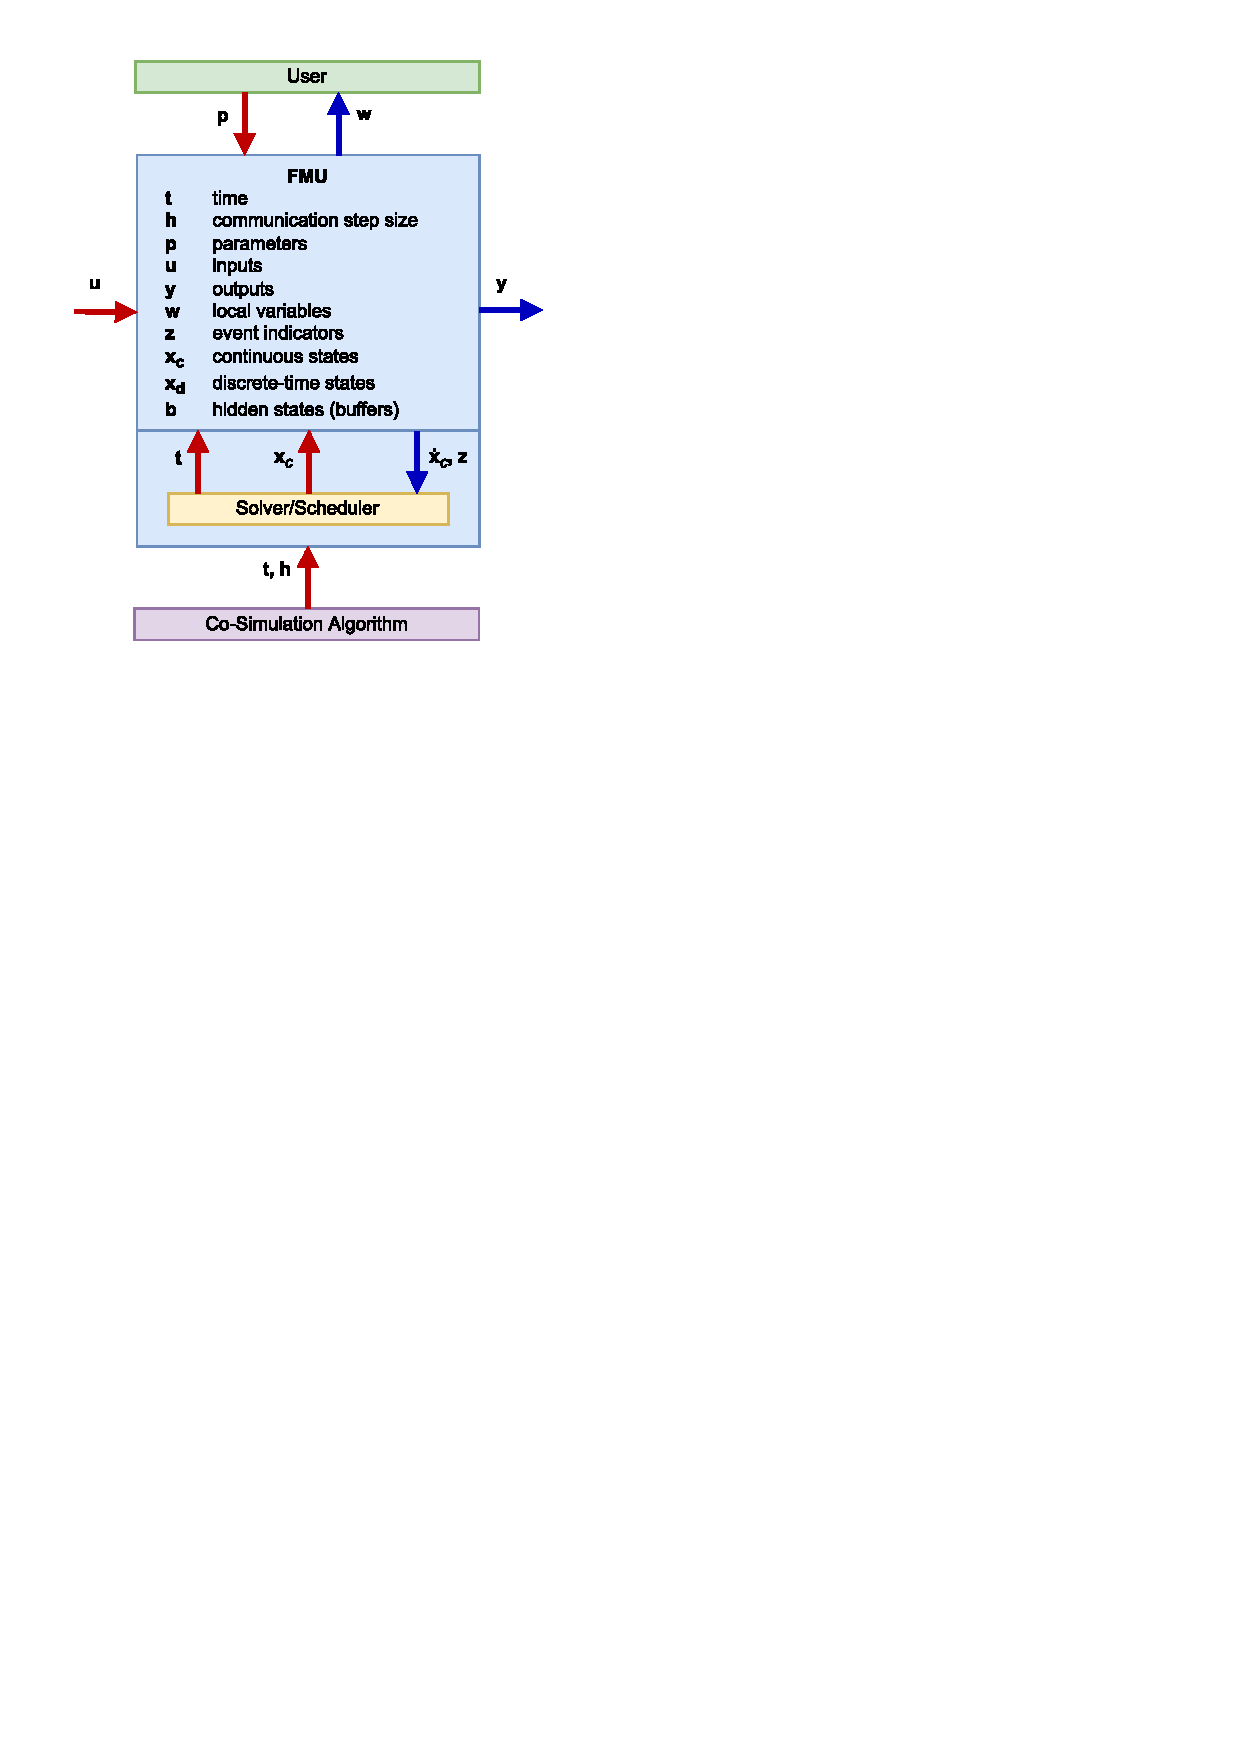
\includegraphics[scale=0.6]{figures/fmi_cs.pdf}
    \caption[FMI for model exchange (left), and FMI for co-simulation (right)] {FMI for model exchange (left), and FMI for co-simulation (right) \cite{fmidoc}}
    \label{fig:fmi}
\end{figure}

In short, CAPE-OPEN is a standard of a component-based approach to process simulation \cite{Belaud2002}, especially addressing the chemical manufacturing domain. The standard can be seen as having two parts. The first is Process Modelling Components (PMC), they represent functionally separated building blocks such as thermodynamic and physical properties engines, or numerical solvers that compute highly nonlinear equations which arise from the flowsheet. The second one, Process Modelling Environment (PME), is essentially a flowsheet---a common diagram used by chemical engineers to indicate the flow of plant processes and equipments---that utilizes services from PMCs, and is supposed to handle the related connections seamlessly. CAPE-OPEN compliant simulations made by different vendors are able to maintain consistent interoperability without ``glue code" or other manually coded wrappers. 

While CAPE-OPEN primarily pertains to the chemical industry, FMI is applicable to more general Cyber-Physical Systems (CPS). FMI handles the interfacing of functional mock-up units (FMU), which is the encapsulation of a model in XML format. The XML schema could contain model variables, time-step information, etc. The APIs of the FMI and the specifications of the FMU depend on the choice of interface types. There are currently three types, which are model exchange, co-simulation, and scheduled execution. Since the third type is relatively new---introduced in FMI 3.0---it has not been fully supported by many development environments, thus we will focus on the first two types. They are described as follows (see also Figure \ref{fig:fmi}): 

\begin{itemize}

  \item Model Exchange: exposes a numerical algorithm (e.g. ODE) to an external solver of an importer (the simulation environment). Using this solver, the FMU is evaluated at a specific time instant.
  
  \item Co-Simulation: implements not only the model algorithm, but also the required solution method. The data exchange between FMUs is restricted to discrete communication points, thus the co-simulation algorithm (serving as the master algorithm) is shielded from how individual FMUs advance time internally.

\end{itemize}

In brief, CAPE-OPEN targets a specialized domain, in this case, the bio-chemistry production. FMI is more generic such that it addresses to a wider range of models. Both approaches are valuable to the DT developer as different DT services may include a narrow set of model domains, or they could utilize models from considerably diverse disciplines.

\subsection{Orchestration} \label{sec:orch}
This subsection covers four distinctive approaching styles for orchestration:
\begin{itemize}

\item General-purpose modeling language.

\item Development-and-Operations (DevOps).

\item Service-orientated architecture (SOA).

\item Actor-orientated model.


\end{itemize}

The styles are deliberately chosen because they originate from different software domains. We welcome the diversity because it helps to find out what strategies are suitable for further developing as a framework for our DT. A general-purpose modeling language such as Systems Modeling Language (SysML) \cite{sysml} is crucial for system engineers to convey designs. The DevOps paradigm is based on the increasing demands of rapid software production by business enterprises. SOA is adopted broadly in cloud computing and IoT applications. Finally, an actor-orientated model like Ptolemy II \cite{ptolemy} is inspired by the proliferation of CPSes which is followed by the desire for an experimentation platform.

\subsubsection{General-purpose modeling language}

As general-purpose modeling language, Unified Modeling Language (UML) and SysML are two of the more well-known ones. In fact, SysML is a dialect of UML targeting especially MDSE applications, which makes it more relevant under the DT context. SysML---and UML, to a vast extent---emphasizes in providing rich static and dynamic behavioral information in the form of diagrams. To gain an idea of how SysML can describe interactions of a complex system, we summarize its taxonomy in Figure \ref{fig:sysmltax}.

\begin{figure}[hbt!]
  \centering
  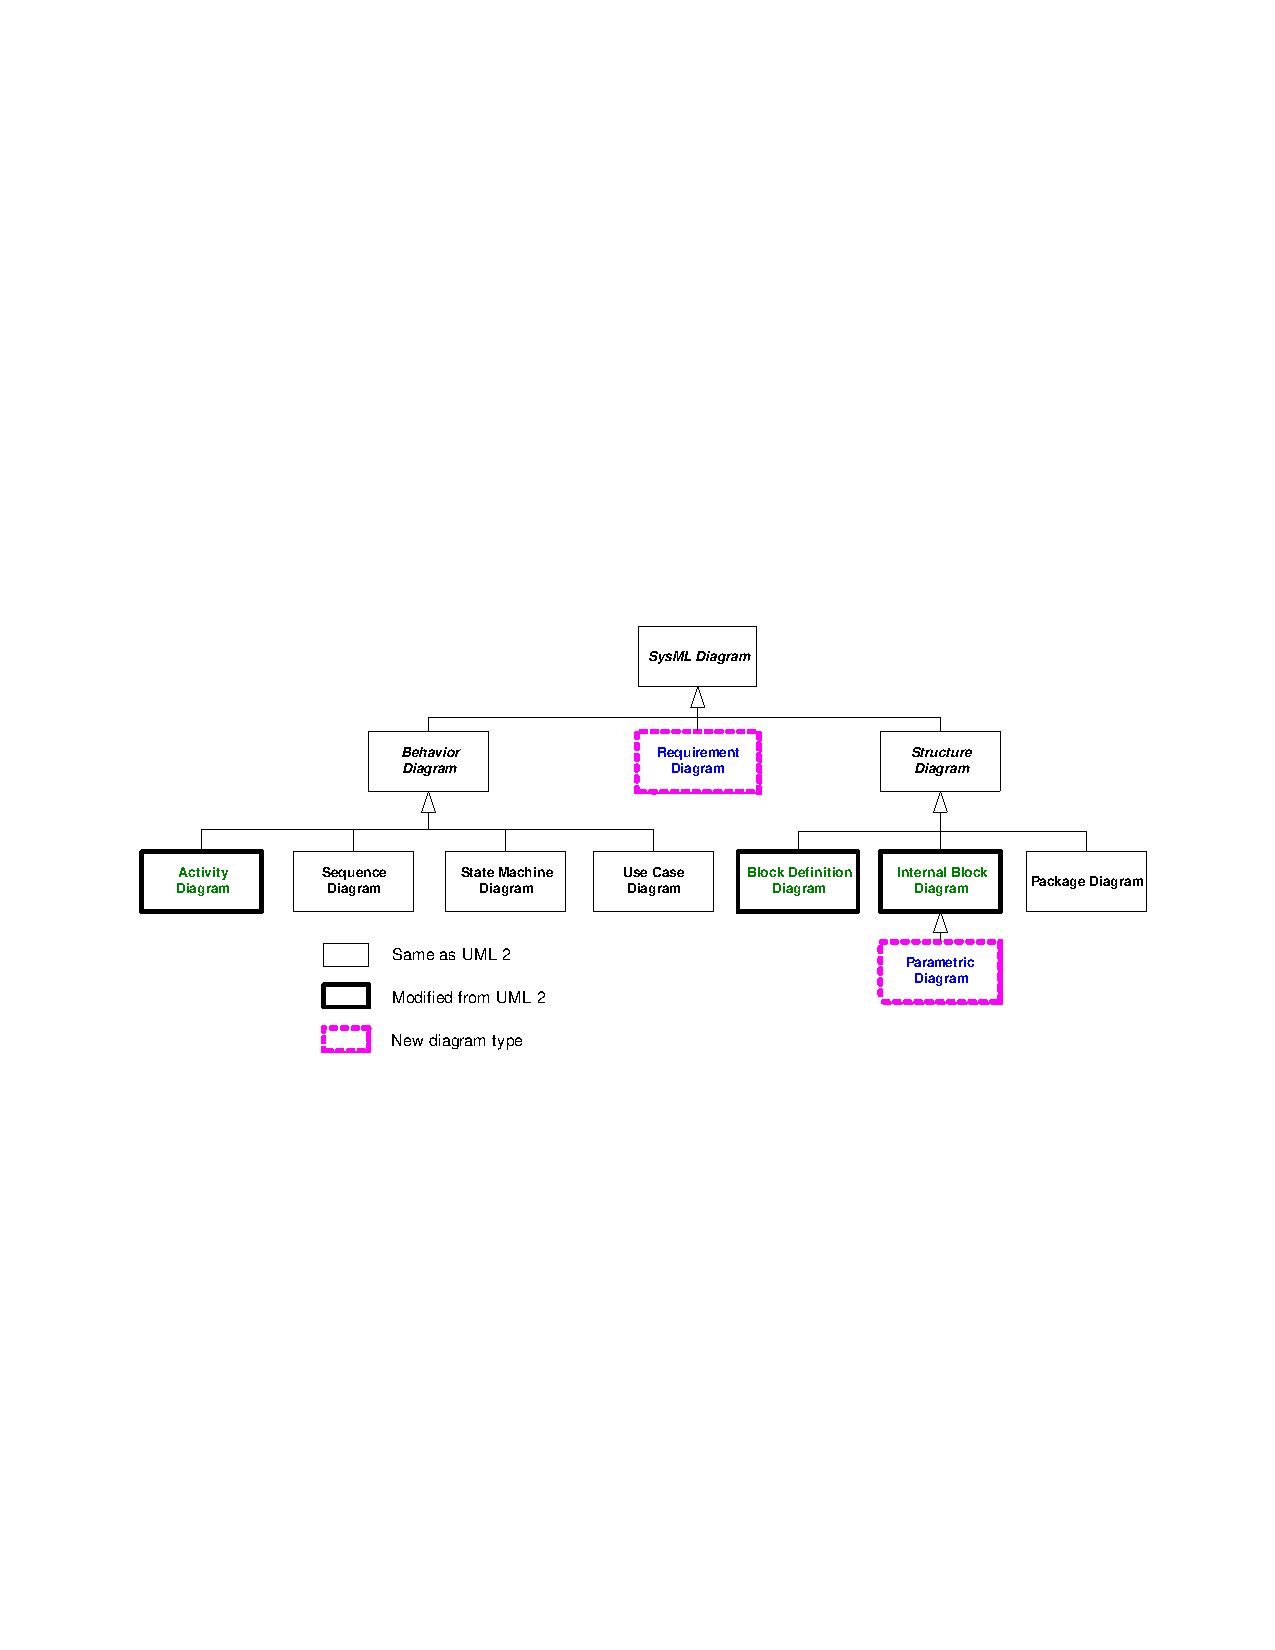
\includegraphics[scale=0.75]{figures/sysml_tax.pdf}
  \caption[SysML diagram taxonomy]{SysML diagram taxonomy \cite{sysmlspec}}
  \label{fig:sysmltax}
\end{figure}

The structure (static) diagrams can represent the system structures in varying degrees of transparency, for instance, Block Definition (black-box), Internal Block (white-box), or Requirement (declarative). The behavior (dynamic) diagrams represent the interactions of internal parts. For example, Activity Diagram describes the flow and the decisions of the component processes. Sequence Diagram extends the precision further by describing the sequence of the processes and what data they propagate in each step. 

The various diagram types in SysML enable the inclusion of system descriptions on different abstraction levels, so throughout all stages of the developmental cycle, the stakeholders---likely from various disciplines---can understand relevant diagrams without much efforts. However, one aspect SysML does not concentrate on is the ability to coordinate with external toolsets, especially if they do not adhere to the modeling language syntax in the first place. One who wishes to establish a ``live link" to SysML modelling environment from the outside will often find themselves working considerably on a conversion layer. Due to this reason, we incline not to consider it in the framework selection of this project.

SysML is a modelling language, not a framework per se. Yet there exists a number of platforms which utilize SysML to accomplish modelling and design activities, including the orchestration of models within the platform environment; one of them is IBM Rhapsody \cite{IBMSYSML}. This kind of platform inherits the previously mentioned disadvantages of SysML, i.e., cumbersome to incorporate external toolsets that do not adhere to the SysML syntax. However, we find the diagram approach in SysML keeps the execution workflow of the components very well organized. This is an attractive property for orchestration that we would like to have in our DT too.

\subsubsection{DevOps}
DevOps practice has received much attention, attributing to its emphasis on fast provisioning of business processes \cite{Ebert2016}. The core idea is that the development and operation are merged into one continuous loop of forward delivery and feedback (see Figure \ref{fig:devops}), often referred collectively as continuous integration and continuous deployment (CI/CD).

\begin{figure}[hbt!]
  \centering
  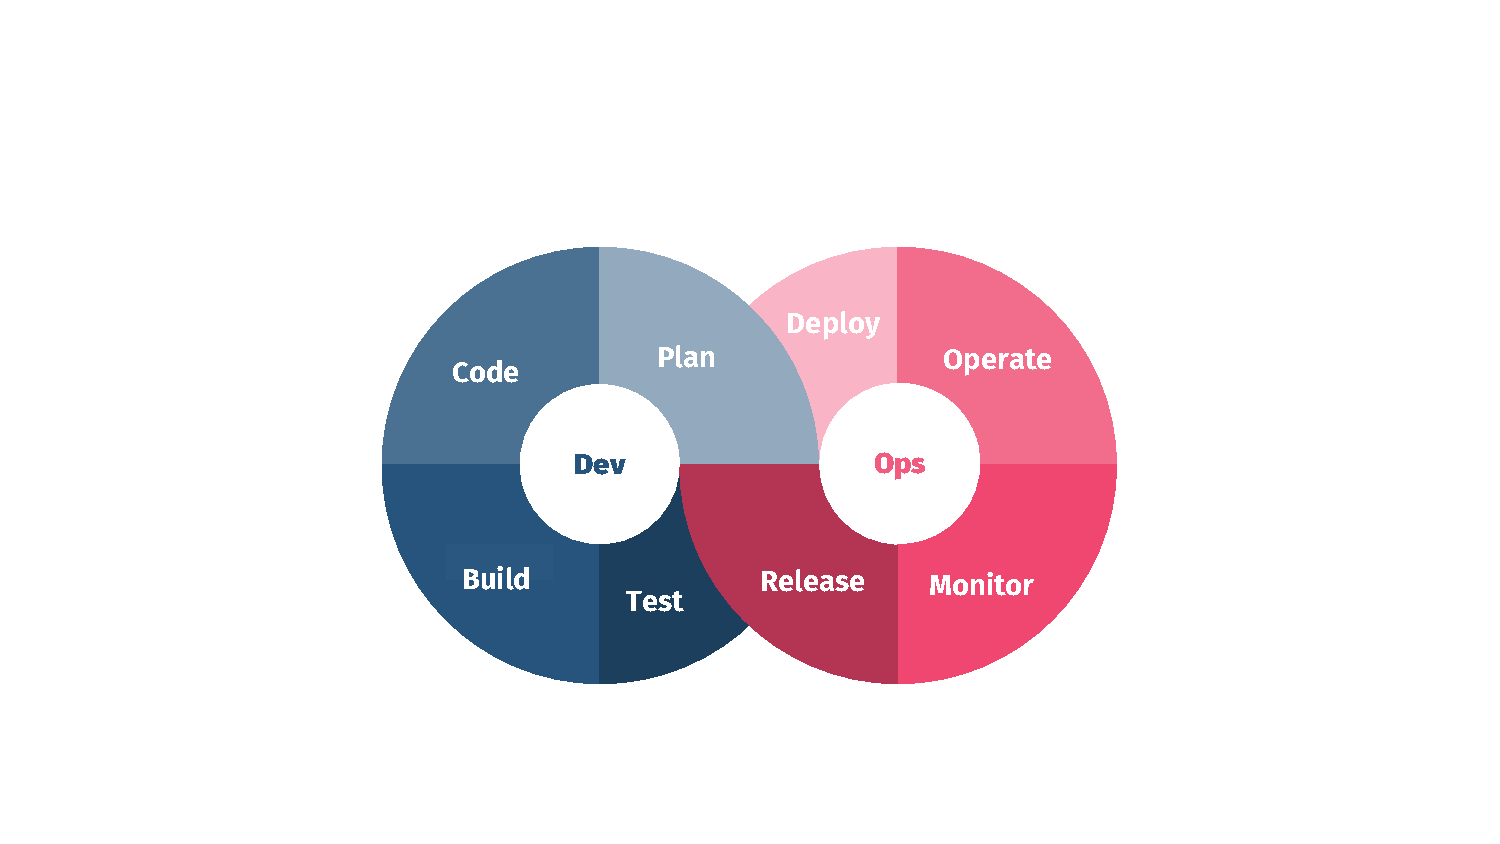
\includegraphics[scale=0.4]{figures/devops.pdf}
  \caption{DevOps concept portrayed by the infinite loop}
  \label{fig:devops}
\end{figure}

\begin{figure}[hbt!]
  \centering
  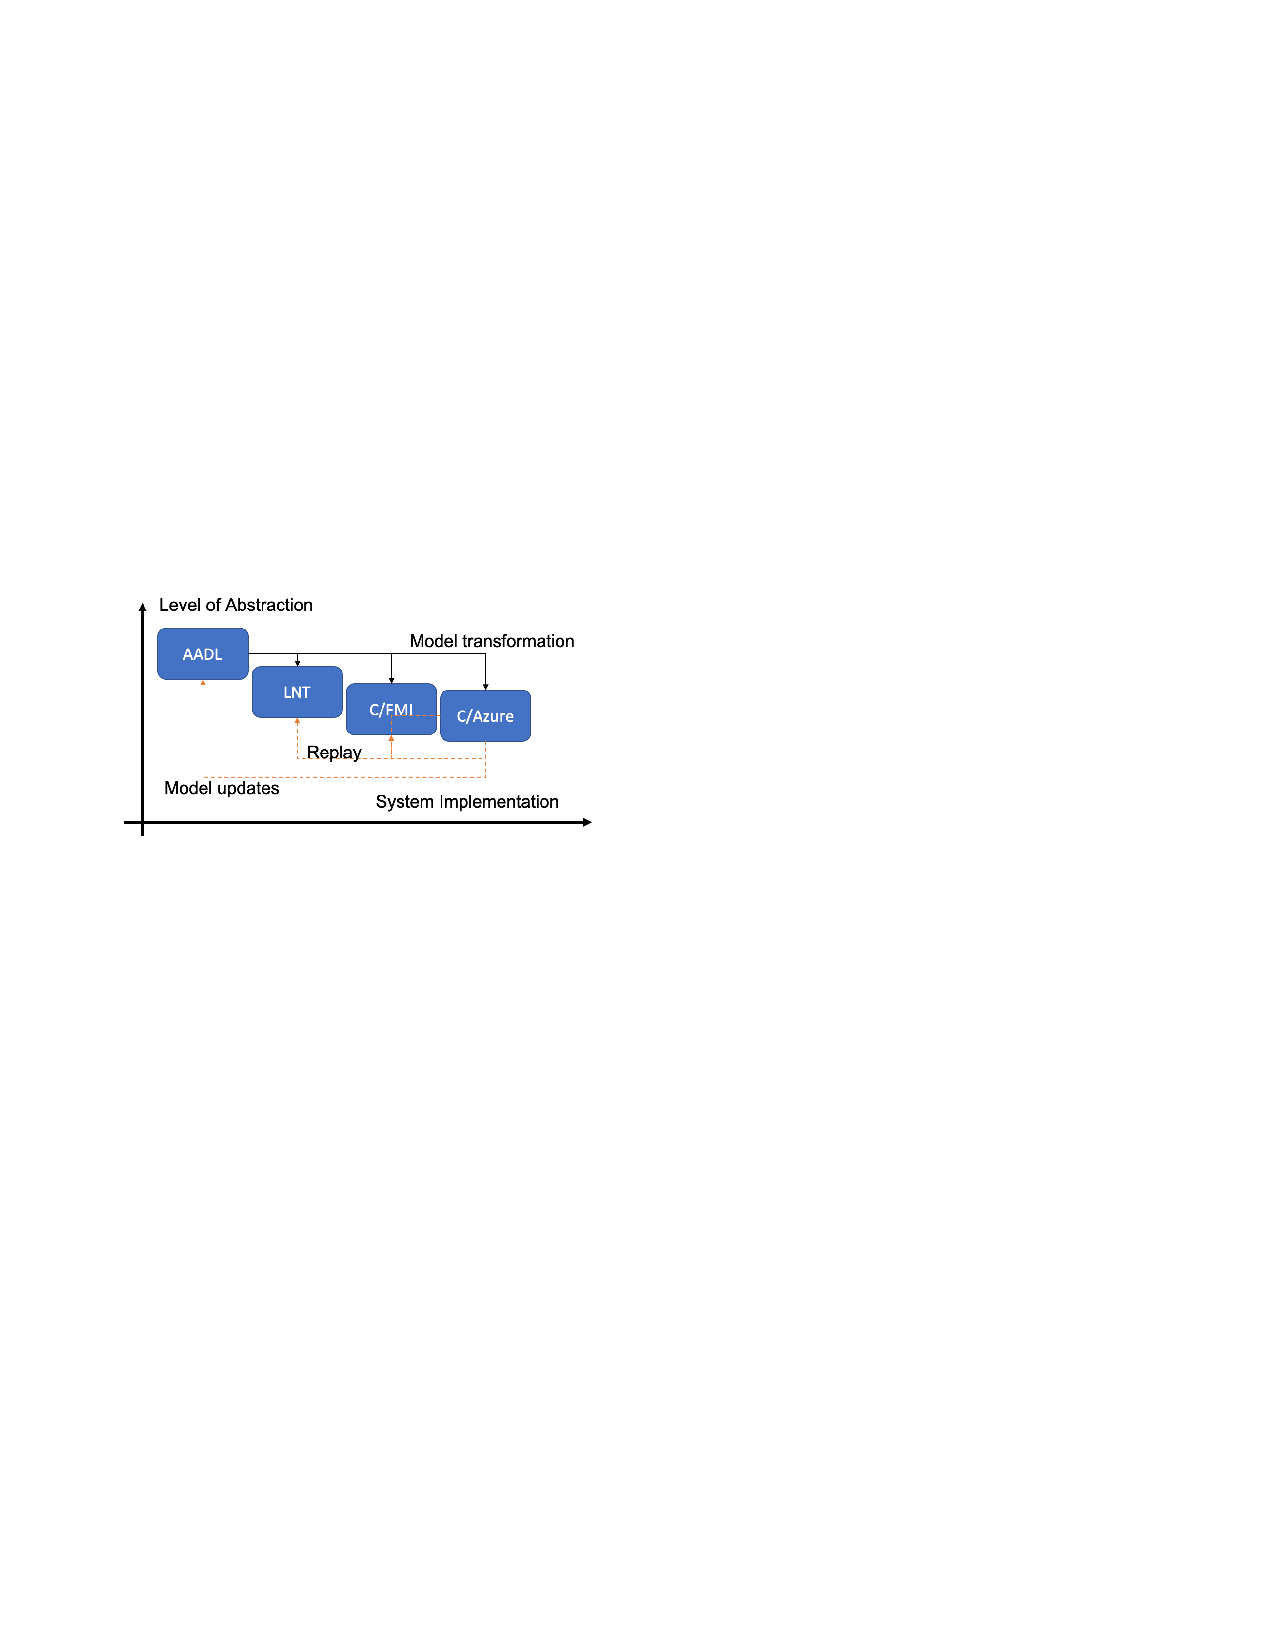
\includegraphics[scale=0.9]{figures/twinopsloop.pdf}
  \caption[TwinOps forward and feedback loop]{TwinOps forward and feedback loop \cite{Hugues2020}}
  \label{fig:twinopsloop}
\end{figure}

Hugues et al. \cite{Hugues2020} borrows this idea and proposes a DT variant of DevOps called TwinOps. In TwinOps, the ``Dev" part transcends to DT model integration and target code generation; and the ``Ops" part is overloaded with data collection and analysis in DTs. As illustrated in Figure \ref{fig:twinopsloop}, the black arrows are the code generation forwarded to various targets, and the orange arrows represent the data analytic feedback. In the work of Hugues, the exemplified case study of a building monitoring system utilizes the technology stack consisting of AADL, LNT, C, FMI, and Azure to build a pipeline. The AADL toolchain is responsible for specifying the modeling architecture as well as requirements. The LNT target enables model-checking. The C/FMI target supports modeling and simulation of the virtual entity. Finally the C/Azure target leverages a containerized cloud system to deploy execution command on the physical entity.

It is worth to note that under the DevOps presumption, the orchestration is implicit in TwinOps. The orchestration is embedded in the CI/CD pipeline for which the user takes the responsibility to configure the steps for transporting and transforming the model states.

TwinOps will be taken as a framework to be investigated further in Chapter \ref{ch:methodology}.

\subsubsection{SOA} 
As cloud services continue to gain popularity, there is a number of studies \cite{Preuveneers2018, Borghesi2021, Hung2022} that look into constructing DTs in line with SOA. In this approach, it regards either the VE models or the services in DTs as independent microservices. The VEs are often deployed as containers, and orchestrated by off-the-shelf applications such as Kubernetes \cite{Kubernetes}, for example, Kubernetes could use DNS for service discovery and exploits network traffic controls for scaling. This view of DTs provides the benefits of rapid deployment, as well as auto monitoring, scaling, and load balancing among other features which are found in commercial cloud services. 

As the number of entities introduced to the existing microservices pool continues growing, we can establish a machine-to-machine (M2M) network. An M2M network is characterized by localized---in the sense of not requiring a powerful computing node from another distant network---exchanges of data and services among the entities. It is contrary to the old-fashioned approach where only one central mainframe responsible for all services. This feature is considered attractive under the DT orchestration context, since DT models are also logically separated; can exchange data and contribute to the services. 

SOA will be the basis of the ThingsBoard framework which we choose to investigate further in this project. More will be discussed in Chapter \ref{ch:methodology}.

\subsubsection{Actor-orientated model}
An actor-orientated model as used by the Ptolemy II framework coordinates actors in various models of computation (MoC) while maintaining strong semantics of each individual model \cite{Ptolemaeus2014}. The term ``actor" refers to a self-contained component in the system that can interface with other components, comparable to the ``object" in object-oriented programming (OOP). The main difference is while OOP objects interface through ``methods", the actors interface primarily through ``ports". The notion of MoC refers to an abstract collection of rules that govern the interaction between components in a design. It is analogous to the ``laws of physic" that are used to describe a given system. Figure \ref{fig:moc} shows\footnote{In the figure, the meanings of the colors were never specified in the original source} a summary of the relationship between MoCs, which are represented as ``domains" in Ptolemy II.

\begin{figure}[htb!]
  \centering
  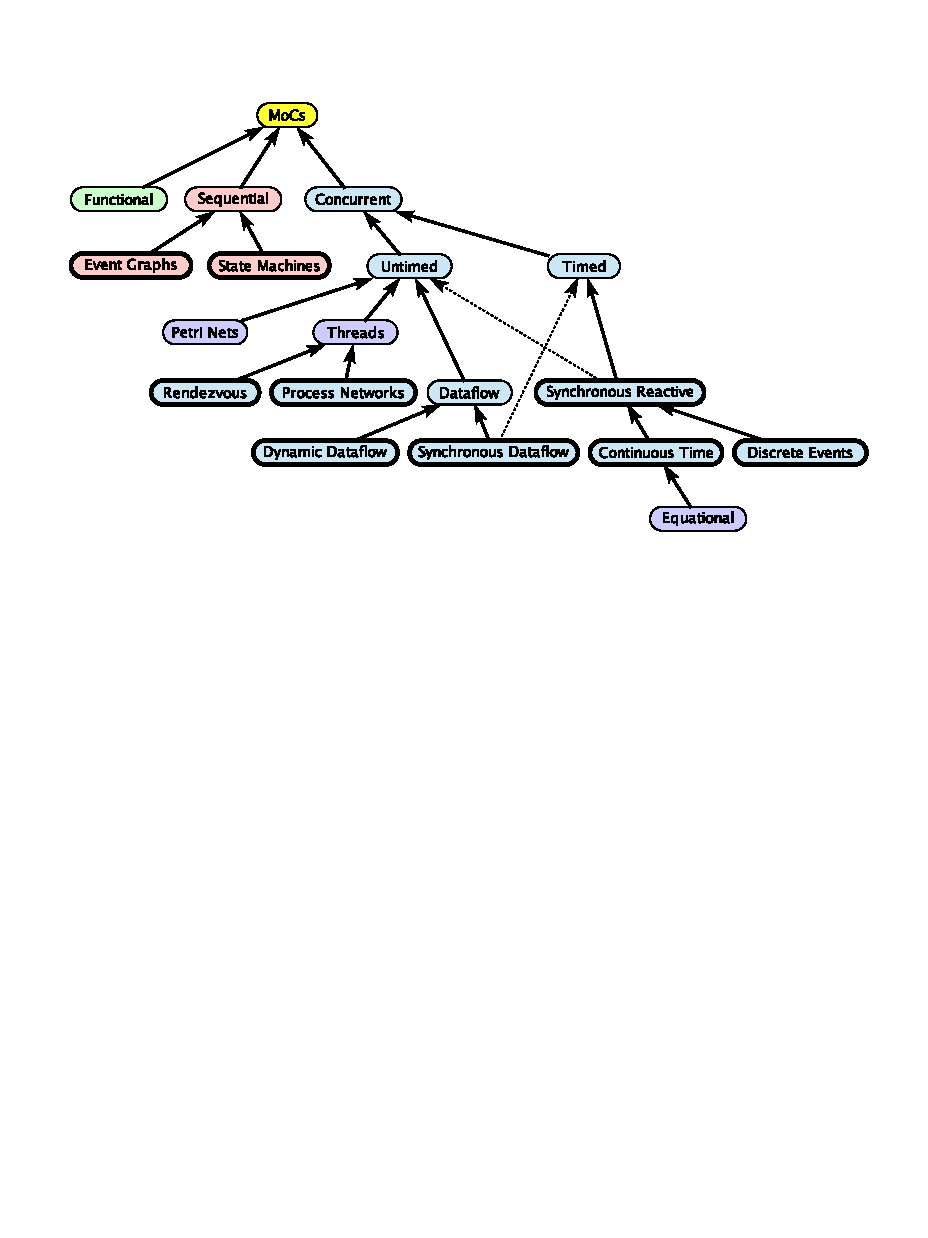
\includegraphics[scale=0.8]{figures/moc.pdf}
  \caption[MoCs relationship]{MoCs relationship \cite{Ptolemaeus2014}. The nodes with thick edges are currently supported by the latest Ptolemy II version. Bold arrows indicate primary associations. Dotted arrows denote alternative associations with either timed or untimed mode.}
  \label{fig:moc}
\end{figure}

We will consider Ptolemy II as one of the frameworks to be investigated further in Chapter \ref{ch:methodology}. Below is a list of some MoCs that we consider more applicable to the DT contexts of manufacturing and production plant:

\begin{itemize}

  \item Process network (PN) \cite{Tripakis2014} : scheduling for concurrent distributed processes. It has a benefit of determinacy as long as there is a unique solution to the balance equations of the nodes within the network. 

  \item Finite state machine (FSM): captures control-dominated behaviors. 
  
  \item Discrete event (DE): suited for modelling the behaviors of complex systems over time, e.g., queuing systems.
  
  \item Continuous time: essential for solving ODEs.

\end{itemize}

\subsection{DT in bioprocessing} \label{sec:dtbio}
In this subsection a number of case studies will be reviewed. They all share the common theme of bioprocess production, which is also shared by the microbrewery DT in our case. We will briefly discuss the integration and orchestration techniques used by these studies.

A study of enzyme production \cite{Mears2017} proposes a model-based strategy to maximize the final fill of a fed-batch process. The study demonstrates a multi-layer approach for orchestration. The cascaded layers are separated by a supervisory layer and a regulatory layer. The supervisory layer implements a mechanistic model that calculates the required start fill. This is the model-based batch planning for initial conditions. The model's parameters are re-fitted using a least squares approach. As for the regulatory layer, the calculated feed rate is adjusted by a PID controller. The results show that orchestrating an additional layer makes the final yield more predictable, which in turn makes the downstream resource allocation easier to manage.

Lopez et al. \cite{Lopez2020} propose a DT of ethanol fermentation. The researchers use a data-driven soft sensor that takes the online spectroscopy measurements to compute the glucose  concentration---referred as process variable (PV)---in real-time. PV is then used as the input to a PID algorithm in order to generate a final control signal---referred as manipulated variable (MV)--- that adjusts the feed rate of the controlled pump. The PV-MV transformation in this example showcases how monitoring models and controlling models can be integrated.

In their manufacturing platform for antibodies, Feidl et al. \cite{Feidl2020} manage to build a process‐wide control with a SCADA system. The system collects unit-relevant data streams from each process unit, then converts to a centralized data storage, which contextualizes and adds a timestamp to each data point, in which the data is transformed to process-relevant. Afterward, the SCADA system is able to send newly determined setpoints to the respective local control units. Hence, an automated end‐to‐end integration of the supervisory control with the data acquisition system is achieved. 

Eppinger and colleagues from Siemens \cite{Eppinger2021} design a DT for ketchup production. The control objectives are evaluated by a set of Key Performance Indicators (KPI). The DT firstly obtains the model parameters from historical data through a machine learning based analysis. A hybrid model that combines an equation-driven model and a data-driven model is then developed before being applied a model order reduction process, such that it can be made compatible with the real-time hard sensors. Once the reduced model is generated, the soft sensors---referred as virtual sensors---can be synthesized and be used to predict the KPIs. Finally, given all available information, the agent of the reinforcement learning algorithm executes actions toward the physical plant and tunes itself with respect to target KPIs by using feedbacks. This study explains a method to orchestrate hybrid models under time critical constraints. 

\section{Summary}
In Section \ref{sec:sota} we surveyed the recent development of DTs regarding monitoring, modelling, and controlling. They are not directly within the topics of integration and orchestration, but the information will be helpful in choosing technologies for our DT building blocks. Besides, some properties of integration and orchestration in fact arise under the influences of these aspects, as they are arguably the backbone of all DT services.

In Section \ref{sec:relatedwork}, we described the approaches for integration, the approaches for orchestration, and multiple DT case studies in the bioprocessing domain, in that order. For integration standards, we presented CAPE-OPEN and FMI, the former targets bio-chemistry applications, while the latter is more general. For orchestration strategies, we reviewed four distinctive styles but decided only three are suitable for our DT. The SysML approach, despite its excellence at propagating system-level descriptions, lacks the features for collaborating with external toolsets. 



\clearpage

\chapter{Methodology and Design}\label{ch:methodology}
We have highlighted the close relationship between DTs and MDSE in Section \ref{sec:context}, hence we choose to adopt the steps in MDSE methodology to present our DT system design. Our steps are as follows:

\begin{enumerate}

\item Describe the system context
\item Identify the requirements
\item Describe the use cases
\item Select the frameworks

\end{enumerate}

Before proceeding to the steps, it is worth to show an overview of the DT architecture.

\section{Architecture of the microbrewery DT}\label{sec:5dbrewery}
\begin{figure}[hbt!]
  \centering
  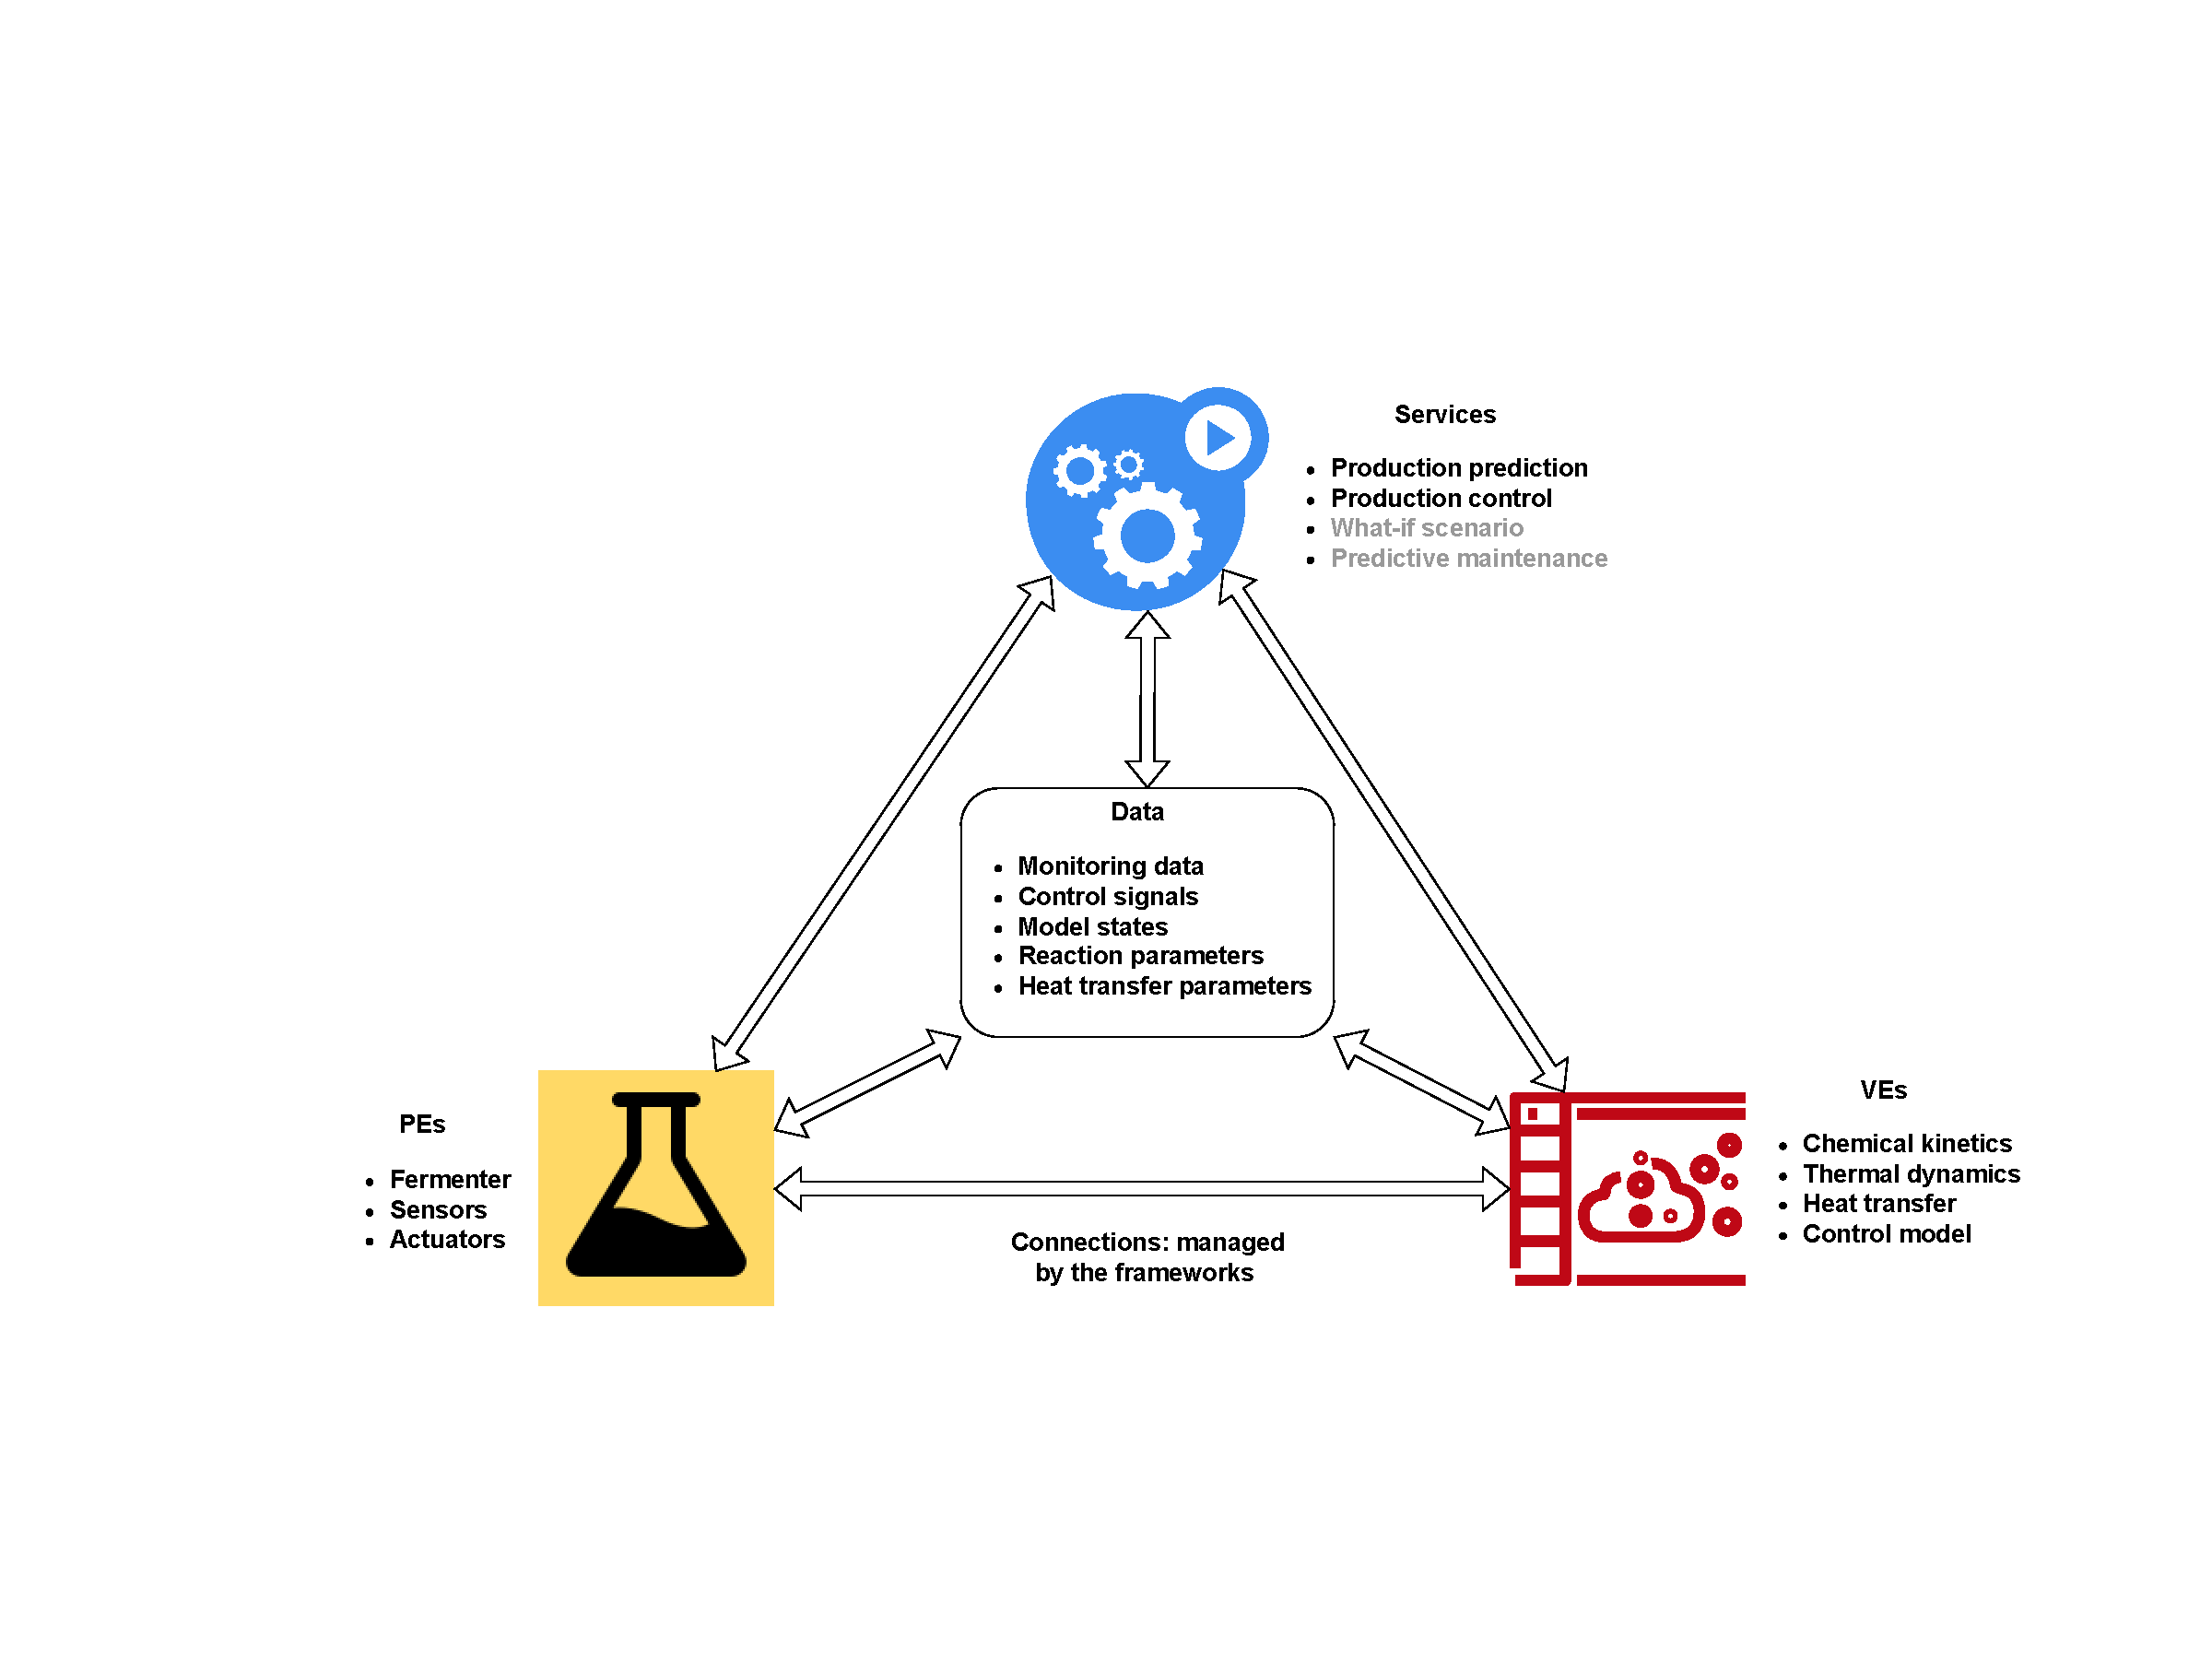
\includegraphics[scale=0.45]{figures/brewery5d.pdf}
  \caption{5D view of the microbrewery DT}
  \label{fig:brewery5d}
\end{figure}

The high level architecture is described using the 5D view (see also Section \ref{sec:overview}), illustrated in Figure \ref{fig:brewery5d}.

\begin{itemize}
  \item \textbf{PEs}: The \textit{fermenter} (also known as bioreactor) is the vessel that holds the wort---the liquid extracted from the mashing process during the brewing of beer. The sensors monitor the temperatures---both inside the fermenter and from the environment, the ambient humidity, and the gravity in the fermenter. The \textit{actuator} is a water pump that can influence the temperature in the system. Appendix \ref{apd:workbench} provides further details of the workbench setup.

  \item \textbf{VEs}: The \textit{chemical kinetics model} is a dynamic model that computes alcohol and yeast concentrations. The \textit{thermal dynamics model} calculates the amount of heat being generated in the system. The \textit{heat transfer model} predicts the future wort temperature. Finally the \textit{control model} produces commands for the actuator in order to alter the temperature to a target value.
  
  \item \textbf{Services}:
  	\begin{itemize}
  	\item \textbf{Production prediction (S1)}: predict the properties of end-product and whether its quantity and quality will meet the demand based on the given materials and resources. 

  	\item \textbf{Production control (S2)}: organize the production schedules and regulate the process such that the utilization of resources is optimized.
  	
  	\item \textbf{What-if scenarios (S3)}: create a hypothetical situation and predict its effect on the production in order to generate variants of the production schedule.
  	
\item \textbf{Predictive maintenance (S4)}: use the data stream from the plant and physical-based modelling to generate a prognosis of the remaining lifetime of plant components.
	\end{itemize}
	
	In order to assess the services and understand the key actors and stakeholders, it is important to recognize their respective phases in the lifecycle. Figure \ref{fig:lifecycle} shows a four-phase lifecycle view \cite{Liu2021} from an industrial perspective and where each proposed service belongs in the cycle.
	\begin{figure}[hbt!]
		\centering
		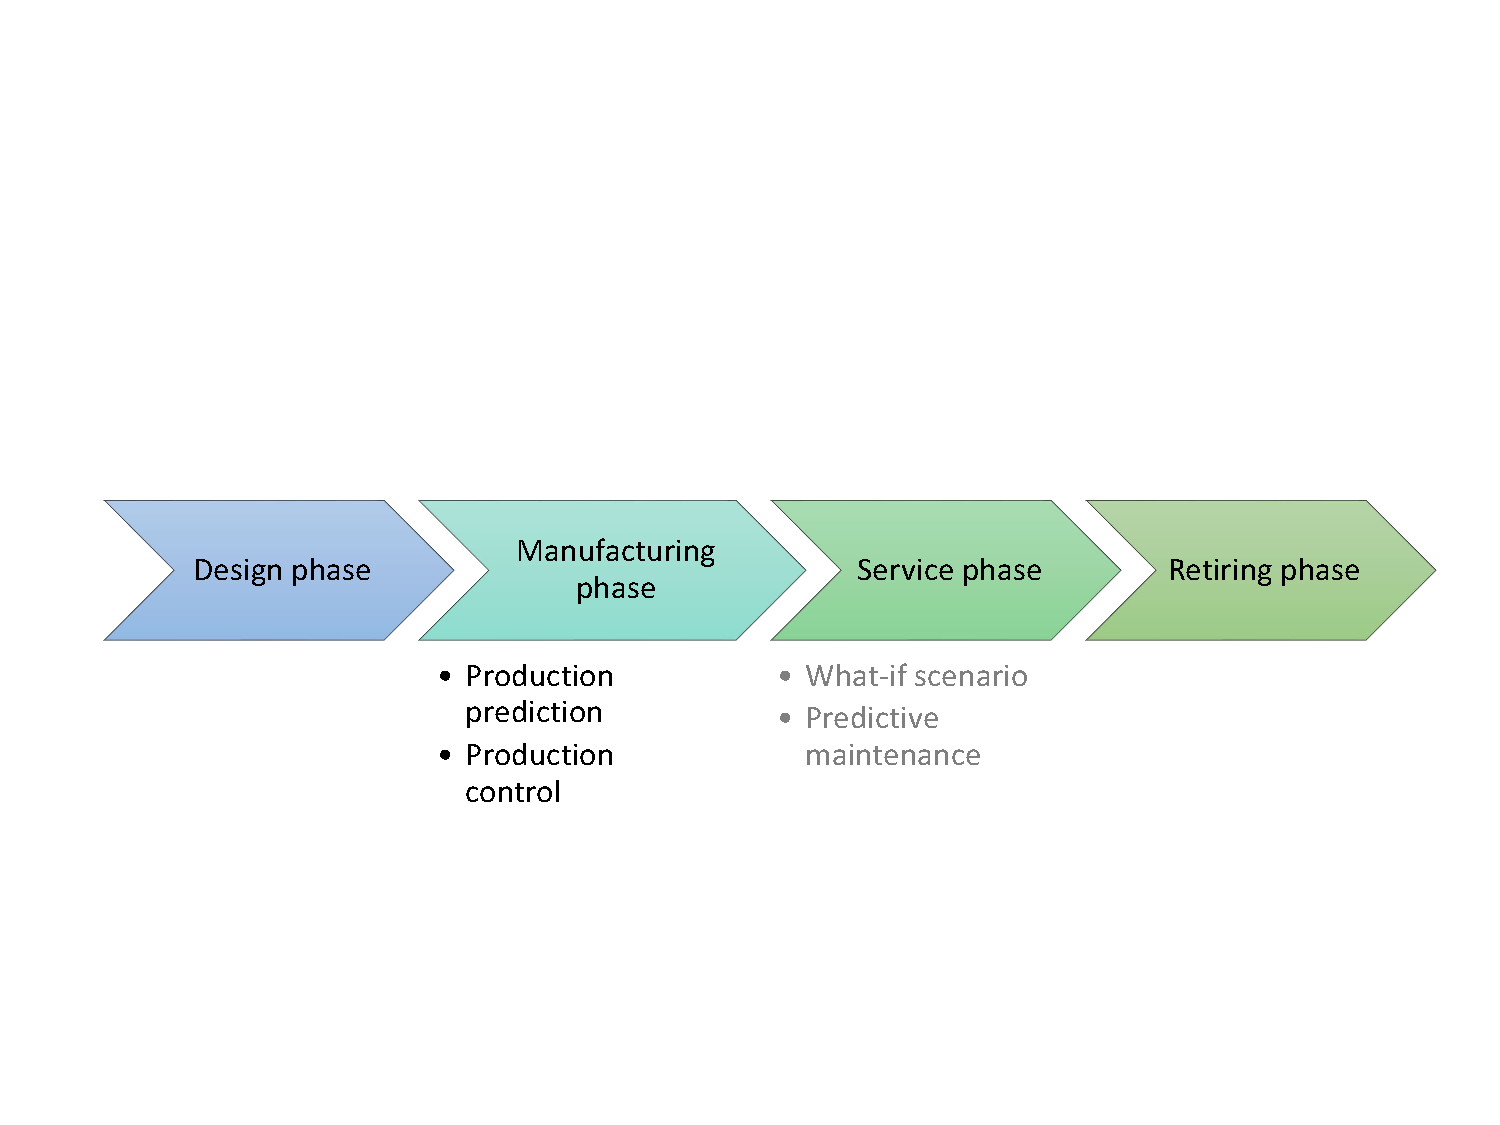
\includegraphics[scale=0.5]{figures/lifecycle.pdf}
		\caption{Services of microbrewery DT in different product lifecycle phases}
		\label{fig:lifecycle}
	\end{figure}
	
The \textit{design phase} encompasses the designs of product, process, and plant, in increasing order of scale. The \textit{manufacturing phase} concerns goods production, and the internal logistical affairs involved. \textbf{S1} and \textbf{S2} primarily concern the questions of production quantity as well as the strategies to optimize the quantity. Therefore, they are considered to be in the manufacturing phase. The \textit{service phase} includes external logistics, user experiences; the detection of anomalies, and repairs. \textbf{S3} and \textbf{S4} fall under this category. In the \textit{retiring phase}, decommissioning of the product is dealt with. Valuable data and parts can be obtained from this recycling action so as to improve the future lifecycles.

Due to the stringent timeline, we only implement \textbf{S1} and \textbf{S2} in this project, reason being that they are considered essential for the brewery operations, and also because \textbf{S3} and \textbf{S4} are, to a considerable extent, based upon the functionalities of the first two services. Nevertheless, we discuss some preliminary designs of \textbf{S3} and \textbf{S4} in the Future work section (Section \ref{sec:futurework}).

  \item \textbf{Data}: The monitoring data are directed from the PEs, and the control signals are directed toward the PE. In the VE space, the \textit{reaction parameters} depend on the chosen beer flavor. The \textit{heat transfer parameters} are the static function of the physical attributes of the fermenter. The remaining data from the VEs are generally denoted as model states. 
   
  \item \textbf{Connections}: They are managed in different fashions by the selected frameworks. More about them will discussed in the later Section \ref{sec:selframe} and Chapter \ref{ch:implementation}.

\end{itemize}

\section{System context description}
Using SysML syntax, the system context is described in Figure \ref{fig:systemcontext} below. The physical components, such as \textbf{Fermenter}, \textbf{Sensors}, and \textbf{WaterPump} are given as the parts of project context.

\begin{itemize}
\item \textbf{DigitalBrewery} is the representation of the microbrewery DT. It makes associations with the other blocks which represent the components of the DT.

\item \textbf{PredictionSystem} and \textbf{ControlSystem} are the embodiments of the VE models and the corresponding services.

\item \textbf{DataManagement} corresponds to the components that manage the storage and the transferring of data.

\item \textbf{I\&O\_Framework} corresponds to the selected integration and orchestration framework in this project. 

\end{itemize}

\begin{figure}[hbt!]
  \centering
  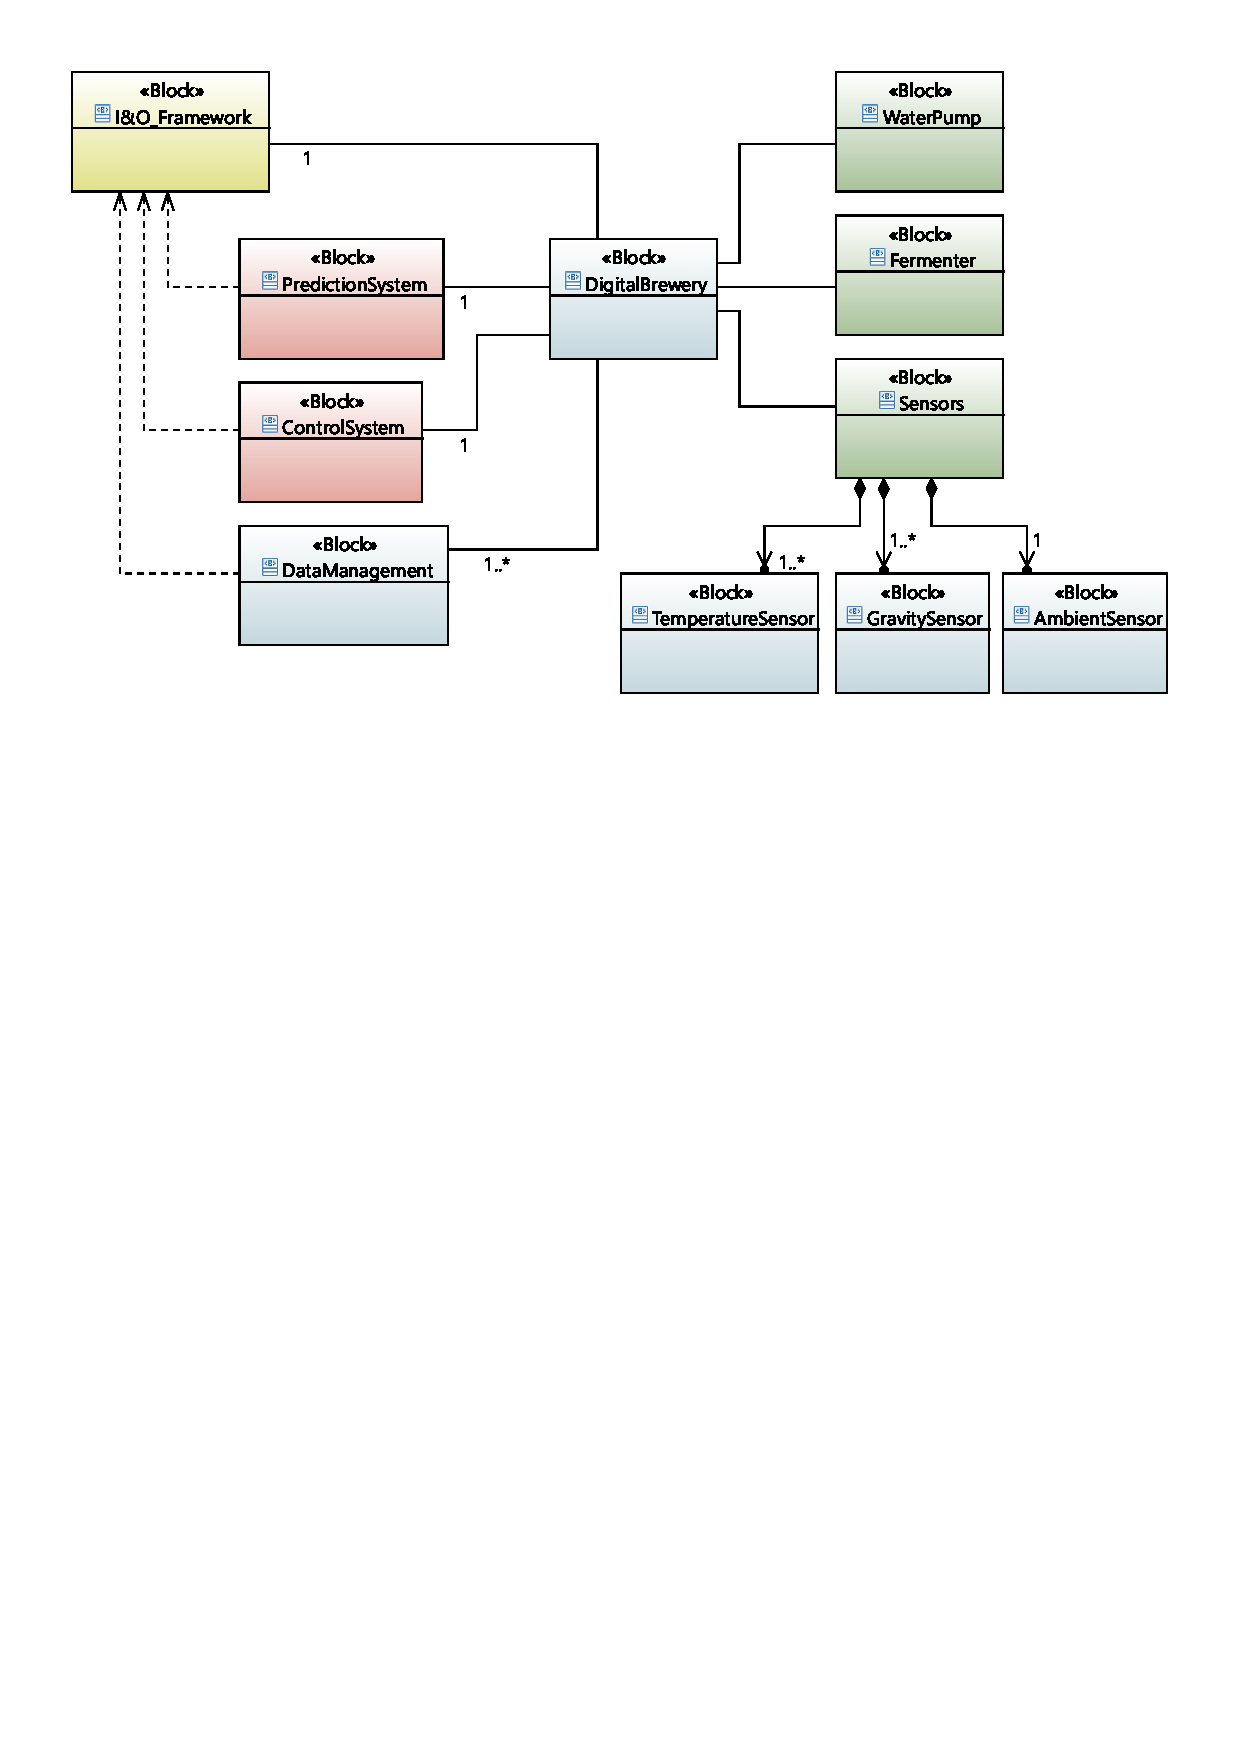
\includegraphics[scale=0.75]{figures/systemcontext.pdf}
  \caption[System context of the brewery DT]{System context of the brewery DT. The PE components are denoted in green. The blocks in red color encompass the services and the process models in VEs. The yellow block represents the integration and orchestration framework.}
  \label{fig:systemcontext}
\end{figure}

\newpage
\section{Requirements identification}\label{ch:req}
\subsubsection{Derivation rationale}
First we highlight a collection of characteristics aligning with the integration and orchestration theme. This collection is gathered based on the high frequency of occurrences found across the literature of bioprocessing DTs. The findings are elicited in Table \ref{tab:iotopics}. Later in this section, these characteristics will become the basis for deriving the requirements of the DT services.

\begin{table}[hbt!]
\centering
\begin{tabular}{|l|l|}
\hline
\textbf{ID} & \textbf{Integration} \\ \hline           
I1 & Configurability of parameters and time advancement \\ \hline
I2 & Automated code/data generation for integration \\ \hline
I3 & Data exchange consistency \\ \hline
I4 & Modularity \\ \hline    
I5 & Ontology checking \\ \hline
\hline                     
   & \textbf{Orchestration} \\ \hline
O1 & Control workflow and execution sequence \\ \hline
O2 & Managing mixed fidelity/granularity \\ \hline
\end{tabular}
\caption{Highlighted characteristics of integration and orchestration}
\label{tab:iotopics}
\end{table}

\textbf{I1} can be further broken down to two parts. First is the adjustability of initialization of the subsystems. As Tolksdorf et al. \cite{Tolksdorf2016} point out, upon the convergence of sub-models into one flowsheet, process engineers often face the challenge of guessing sensible initial values as the sub-models no longer are transparent to them, and a poor guess can easily lead to underperforming models. Therefore, it is argued that the accessibility to critical parameters throughout the whole process is essential to integration. The second part is related to the importance of time step management. In \cite{Neema2014}, the researchers experiment with varying execution step-sizes for a vehicle DT, showing that to a certain degree, distributed components can be ran with different clock rates and still produce matching results. The ability to parameterize time advancement extends flexibility in the platform under design.

\textbf{I2} refers to the required automation to combine models in order to reduce human errors. As chemical process optimizations are rarely accomplished by one single program, manually interfacing multiple simulation packages becomes impractical as soon as the system grows large \cite{Krone2020}. A systematic method to generate ``glue code' including data adaptation is an ideal solution. In practice, we tend to consider a hybrid scheme with varying levels of automation as realistic, as full automation could be too difficult to achieve.

\textbf{I3} suggests in the case when a variable is transferred from one model to another, it shall retain its structure and its dependency relation with other objects. An important implication of this property occurs when several solvers are working on shared data. If information about algebraic dependencies between outputs and inputs is supplied, the importing tool is able to detect and handle algebraic loops automatically \cite{Blochwitz2011}.
 
In \textbf{I4} the modularity property implies not only the plug-and-play accessibility of the models, but also the support for templates---static reuse of resources---and instances---dynamic reuse of resources. Actor-oriented design orthogonalizes component definition and component composition, allowing them to be considered independently \cite{Lee2004}. It promotes modularity which in turn reduces the associated design costs. 

\textbf{I5} considers ontologies. An ontology is the  explicit organization of constituent concepts and the relations between those concepts. More specifically, an ontology can help to express the intended use of a model. In \cite{Ptolemaeus2014}, it is indicated that errors may arise from ontology inconsistencies, as illustrated in Figure \ref{fig:o2ont}.

\begin{figure}[hbt!]
  \centering
  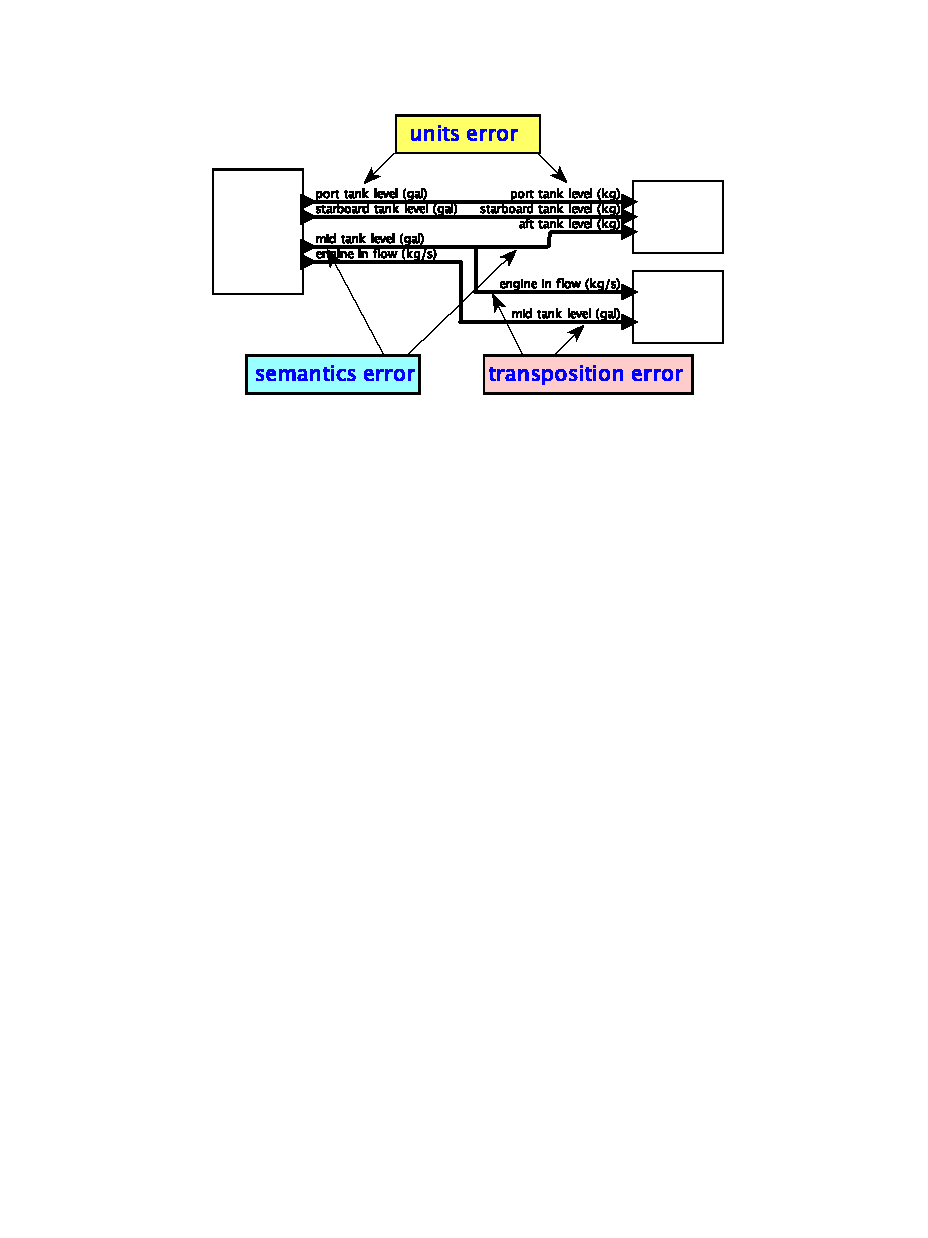
\includegraphics[scale=0.9]{figures/o2ont.pdf}
  \caption[Errors that can be detected by ontology checking]{Errors that can be detected by ontology checking  \cite{Ptolemaeus2014}}
  \label{fig:o2ont}
\end{figure}

\newpage
\textbf{O1} reinforces the importance of effective scheduling. One of the key factors that influences the workflow between models is coupling \cite{Karolius2018}, that is, how tightly are models intertwined with one another. A loose coupling relation generally requires less complex schedules. One may use strategies such as using an external framework to de-couple a pair of inherently coupled models. Other considerations, such as atomicity, might be required should there be concurrent processes.

\textbf{O2} concerns time synchronization and convergence across different models. For instance, merging discrete and continuous time granularities by techniques of sampling and quantization; another example, signaling between time and untimed models. In the case of FMI, an event instant may be driven by a predefined time event or at the transition of state event indicators \cite{Blochwitz2011}. This is to allow numerical robustness, and is a part of the FMI feature which is known as ``hybrid ODE".

The mixed fidelity of data implies varying levels of accuracy in which models' data to quantify the system. This property is often correlated to the computational intensity used by the models. The discrepancy may be solved by data manipulation techniques such as interpolating missing data or sampling out redundant data.

\subsubsection{Production Prediction (S1) Requirements}
The requirements for Production Prediction service are shown in Table \ref{tab:s1req}. The rightmost column indicates the relevant integration and orchestration characteristics.

In addition to requirements, we elicit a set of KPIs in Table \ref{tab:s1kpi}, whose purpose is to verify the effectiveness of the DT regarding how it satisfies the requirements. In principle, each KPI should be a measurable metric that reflects a certain aspect of system performance or non-functional quality. The KPIs are defined in relation to the specific requirements they address.

\begin{table}[hbt!]
\centering
\begin{tabularx}{\textwidth}{|p{1cm}|X|p{2.5cm}|}
\hline
\multicolumn{3}{|c|}{\textbf{Requirements}} \\
\hline
\textbf{ID} & \textbf{Requirement description} & \textbf{Derived from} \\ 
\hline            
R1 & The model state variables shall be validated with real-time empirical data. & I3, I5, O2 \\ 
\hline
R2 & The operator shall be able to configure the initial model parameters and the model execution scheme. & I1 \\ 
\hline
R3 & The model states shall update automatically based on the latest real-time data. & I2, I3, O1 \\ 
\hline
R4 & The model may be queried for its past states in order to optimize its present parameters. & I1, I4, O1 \\ 
\hline
\end{tabularx}
\caption{S1 requirements}
\label{tab:s1req}
\end{table}

\begin{table}[hbt!]
\centering
\begin{tabularx}{\textwidth}{|p{1cm}|p{2.5cm}|X|p{1.5cm}|}
\hline
\multicolumn{4}{|c|}{\textbf{KPIs}} \\ 
\hline
\textbf{ID} & \textbf{Name} & \textbf{Description} & \textbf{Verifies} \\ 
\hline
KPI1 & Level of automation & What are the manual steps required to support the automation of the validation workflow. & R1, R4 \\ 
\hline
KPI2 & Updating delay & How long does it take to perform model state updates. & R3 \\ 
\hline
KPI3 & Data history & What is the amount of historical data that is available for performing predictions. & R4 \\ 
\hline
KPI4 & Modifiability & What configuration options are accessible for model executions and initial values after startup & R2 \\ 
\hline
\end{tabularx}
\caption{S1 KPIs}
\label{tab:s1kpi}
\end{table}

\subsubsection{Production Control (S2) Requirements}
Table \ref{tab:s2req} and Table \ref{tab:s2kpi} shows the requirements and KPIs respectively for the Production Control service.

\begin{table}[hbt!]
\centering
\begin{tabularx}{\textwidth}{|p{1cm}|X|p{2.5cm}|}
\hline
\multicolumn{3}{|c|}{\textbf{Requirements}} \\
\hline
\textbf{ID} & \textbf{Requirement description} & \textbf{Derived from} \\ 
\hline            
R1 & Model optimization may be triggered on the detected disturbance, time, or plant-wide performance. & I5, O1, O2 \\ 
\hline
R2 & Controller calibration may be triggered on time, or state variables deviation. & I2, I5, O1, O2 \\ 
\hline
R3 & Service shall ensure that the calibrations comply with the controller's desired operating range. & I1, I5, O1 \\ 
\hline 
\end{tabularx}
\caption{S2 requirements}
\label{tab:s2req}
\end{table}

\begin{table}[hbt!]
\begin{tabularx}{\textwidth}{|p{1cm}|p{2cm}|X|p{1.5cm}|}
\hline
\multicolumn{4}{|c|}{\textbf{KPIs}} \\ 
\hline
\textbf{ID} & \textbf{Name} & \textbf{Description} & \textbf{Verifies} \\ 
\hline
KPI1 & Traceability & How accessible is the information which concerns the control-induced transitory behaviors. & R3 \\ 
\hline
KPI2 & Latency & What is the response time of actuator triggering. & R1, R2 \\ 
\hline
\end{tabularx}
\caption{S2 KPIs}
\label{tab:s2kpi}
\end{table}

\section{Use case description}
This section covers the use case description for \textbf{S1} and \textbf{S2}.

Figure \ref{fig:usecase1} illustrates the use case diagram for the \textbf{PredictionSystem}. This is corresponding to S1, Production Prediction service.

\begin{figure}[hbt!]
  \centering
  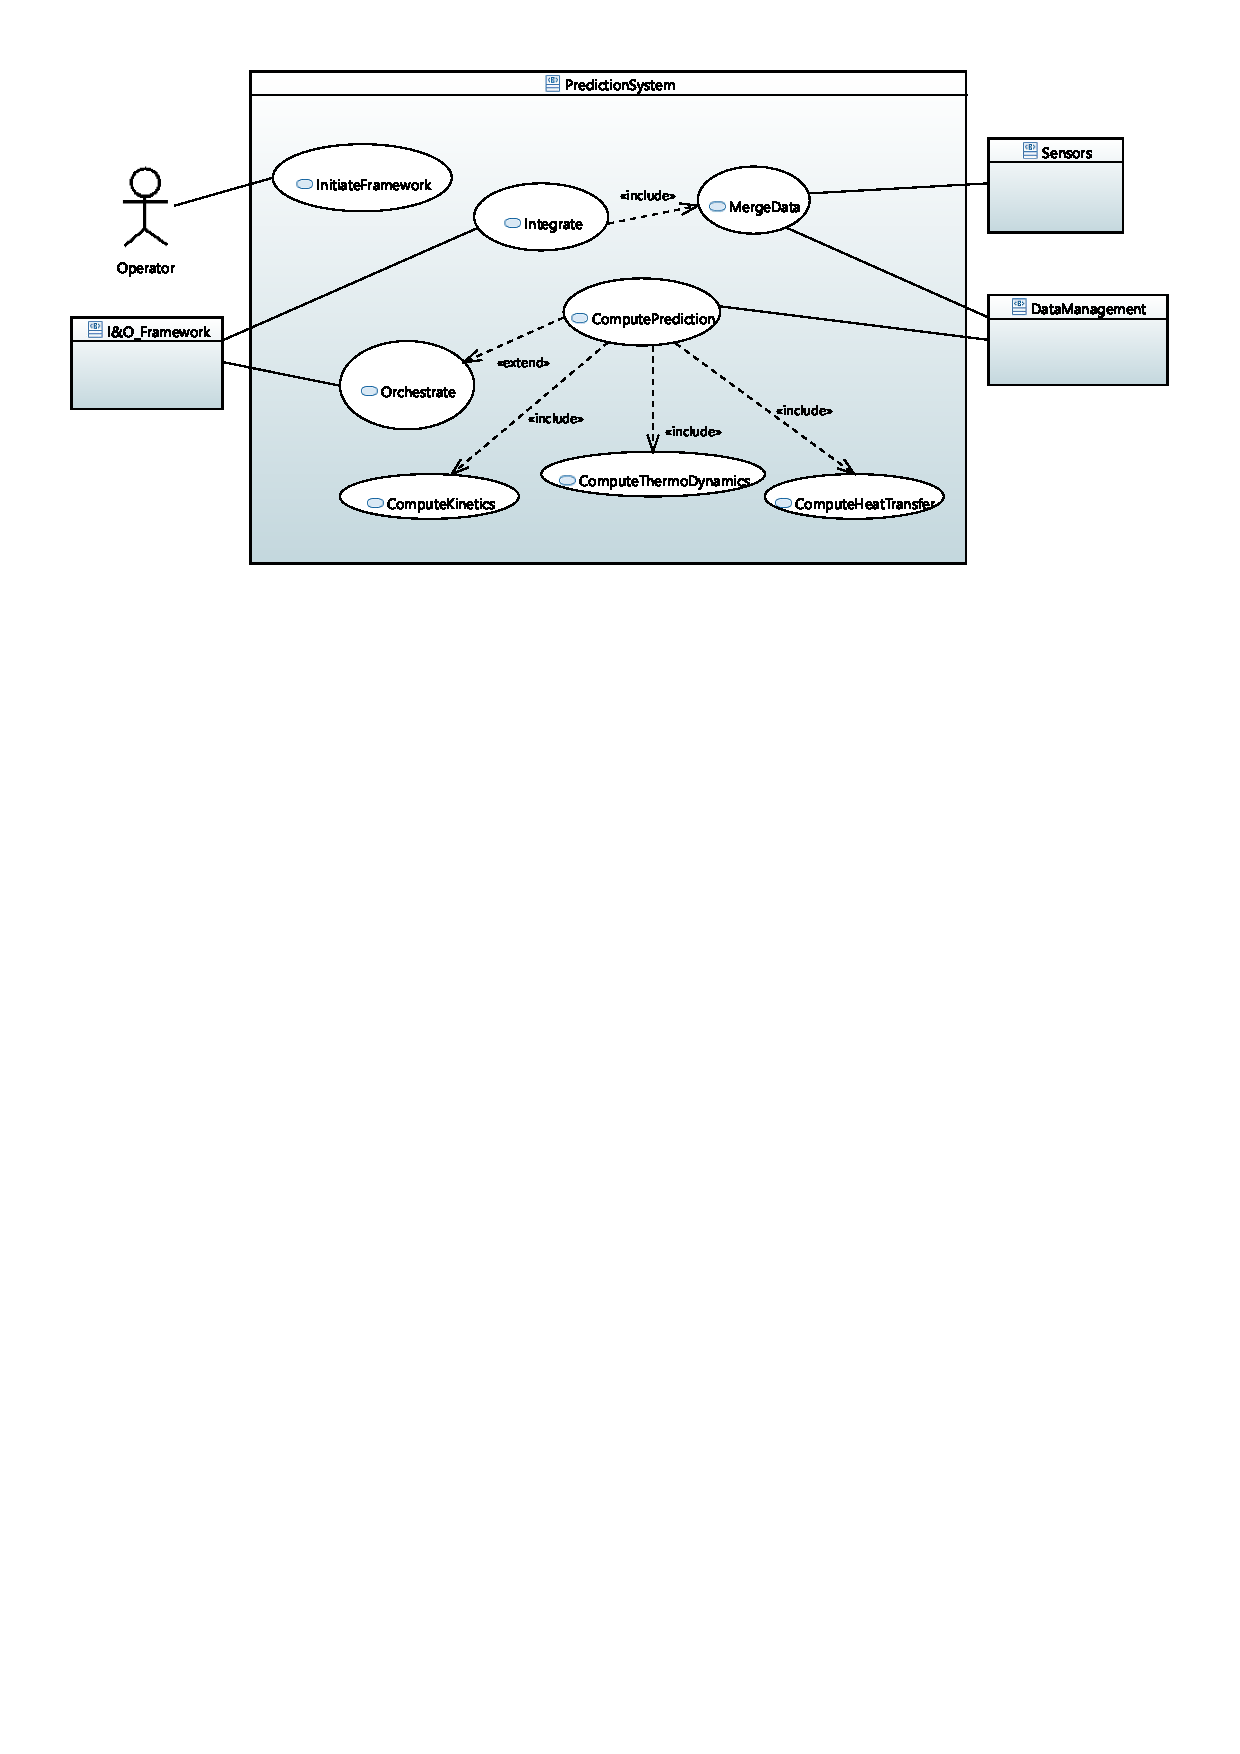
\includegraphics[scale=0.8]{figures/usecase1.pdf}
  \caption{Use cases for S1 scenario}
  \label{fig:usecase1}
\end{figure}

\begin{itemize}
\item In the \textbf{InitiateFramework} use case, \textbf{Operator} accesses the user interface and configures the framework in order to start up the DT.  

\item \textbf{Integrate} manages the data from different sources. It includes \textbf{MergeData} which merges data of the sensors and the model states.

\item \textbf{Orchestrate} manages the scheduling among the models, as well as the validation and updates of the model states.

\item \textbf{ComputePrediction} includes all the calculations in order to generate a prediction value. It includes three use cases that correspond to the VE models of the same name.

\end{itemize}

Figure \ref{fig:usecase2} illustrates the use case diagram for the \textbf{ControlSystem}. This is corresponding to S2, Production Control service.

\begin{figure}[hbt!]
  \centering
  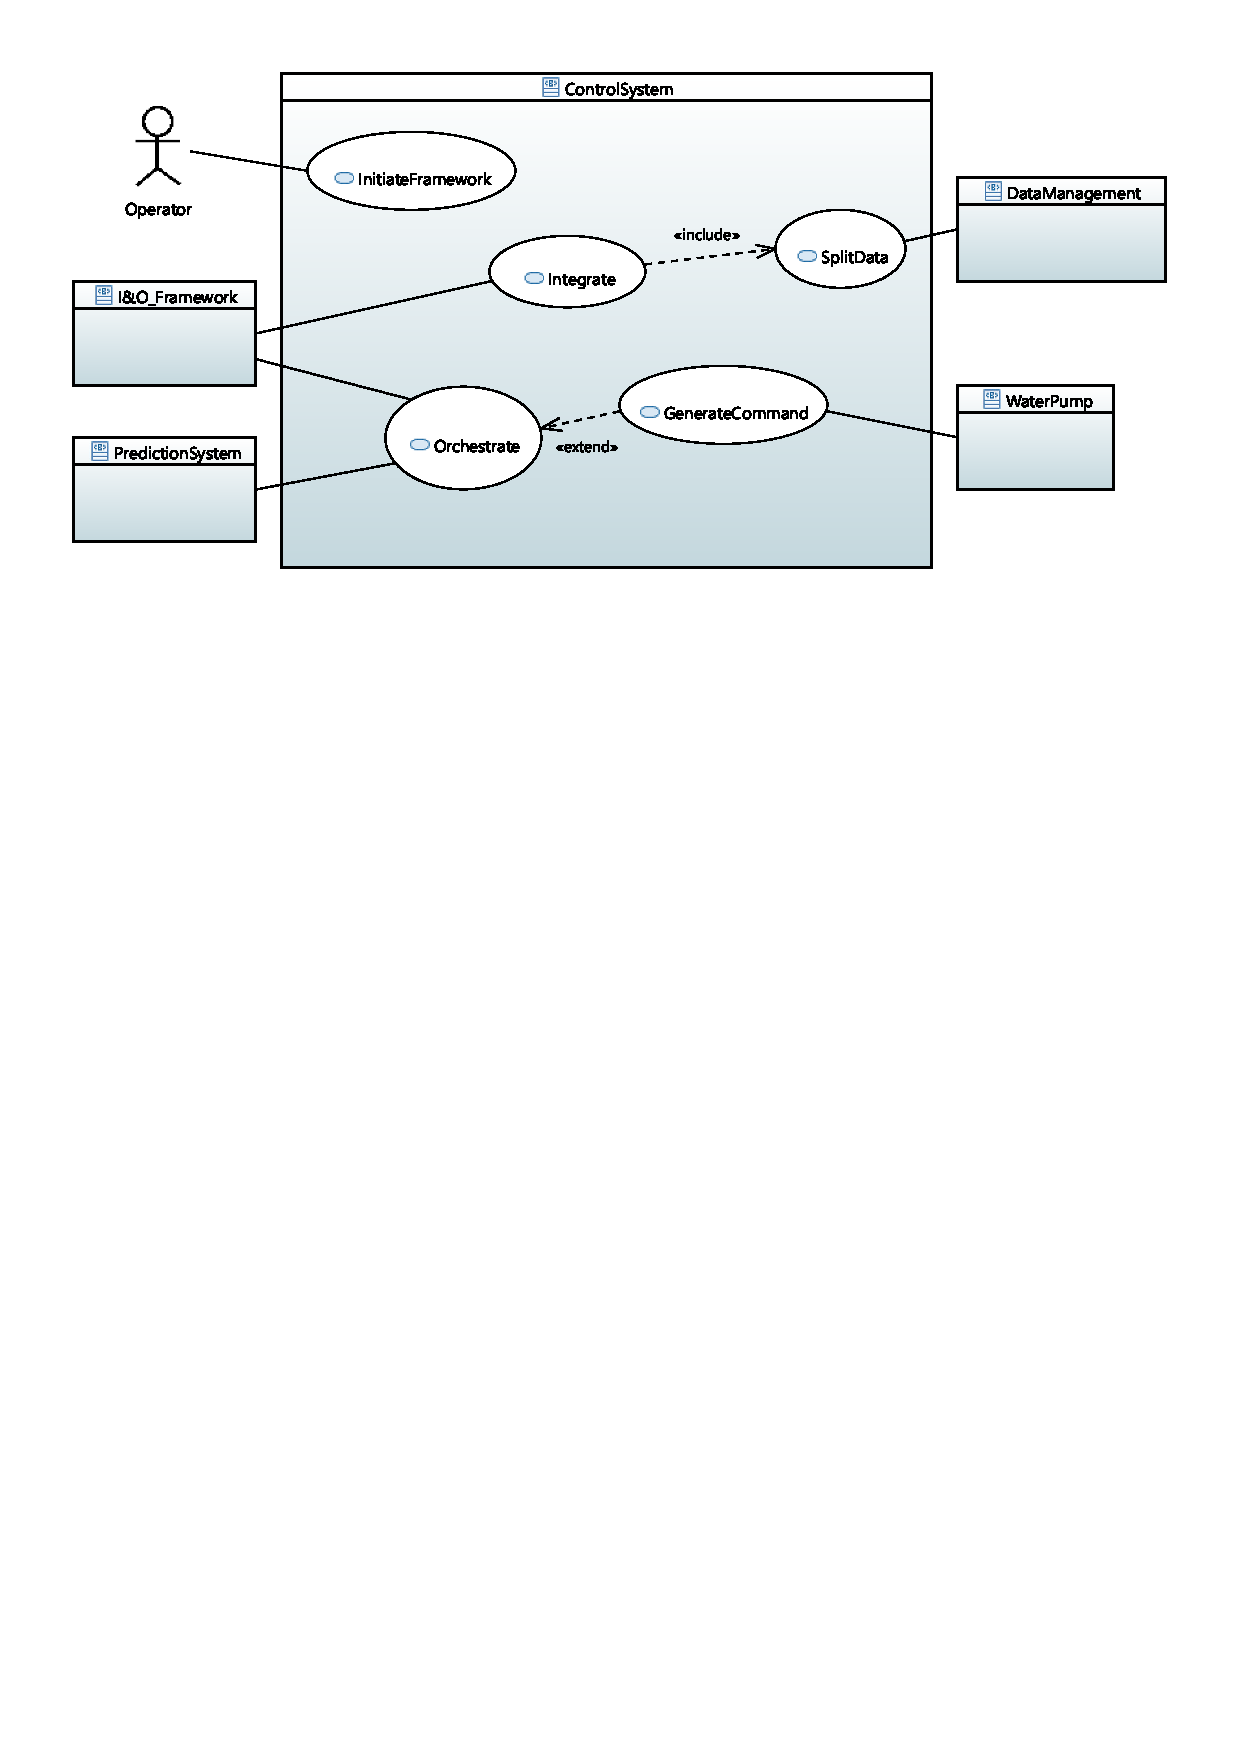
\includegraphics[scale=0.75]{figures/usecase2.pdf}
  \caption{Use cases for S2 scenario}
  \label{fig:usecase2}
\end{figure}

\begin{itemize}
\item \textbf{InitiateFramework}, \textbf{Integrate}, and \textbf{Orchestrate} use cases have the same behaviors as in the S1 scenario.

\item \textbf{SplitData} splits the raw data of control to the right destinations in \textbf{DataManagement}, with the necessary formatting modifications.

\item \textbf{GenerateCommand} uses the control model in VE to generate the control signals to the \textbf{WaterPump}.
\end{itemize}


\section{Selected frameworks} \label{sec:selframe}
This section covers the architecture and workflow of three frameworks, namely, TwinOps, Thingsboard, and Ptolemy II. They are intended for applying integration and orchestration techniques.

These three frameworks are chosen to reflect on the broad spectrum of the software technology sectors, and to highlight the similarity and difference of approaches under the DT context. TwinOps inherits the CI/CD paradigm from DevOps which aims to eliminate the boundary of developments and operations in order to accelerate the software delivery. We argue that this concept can improve the delivery of DT services as well. Thingsboard has its root in the IoT field, which has always regarded the connectivity between ``things" as its core focus. We think this focus can also benefit the connectivity of DT entities. Ptolemy II provides an experimentation platform for CPSes. The management of cyber-objects and physical objects in Ptolemy II is highly applicable to the orchestration and integration of DTs.
 
\subsection{TwinOps} \label{sec:selframe_twop}
The workflow of TwinOps stresses automated transformations, starting at the models in VEs, all the way to the programs running in the PEs. This is also referred as \textit{Model-to-Code-to-Target CI/CD} in the original paper \cite{Hugues2020}. For the feedback direction, the execution traces from PEs are used to validate and update the models, hence closing the pipeline loop. Figure \ref{fig:twinops_workflow} illustrates:

\begin{figure}[hbt!]
  \centering
  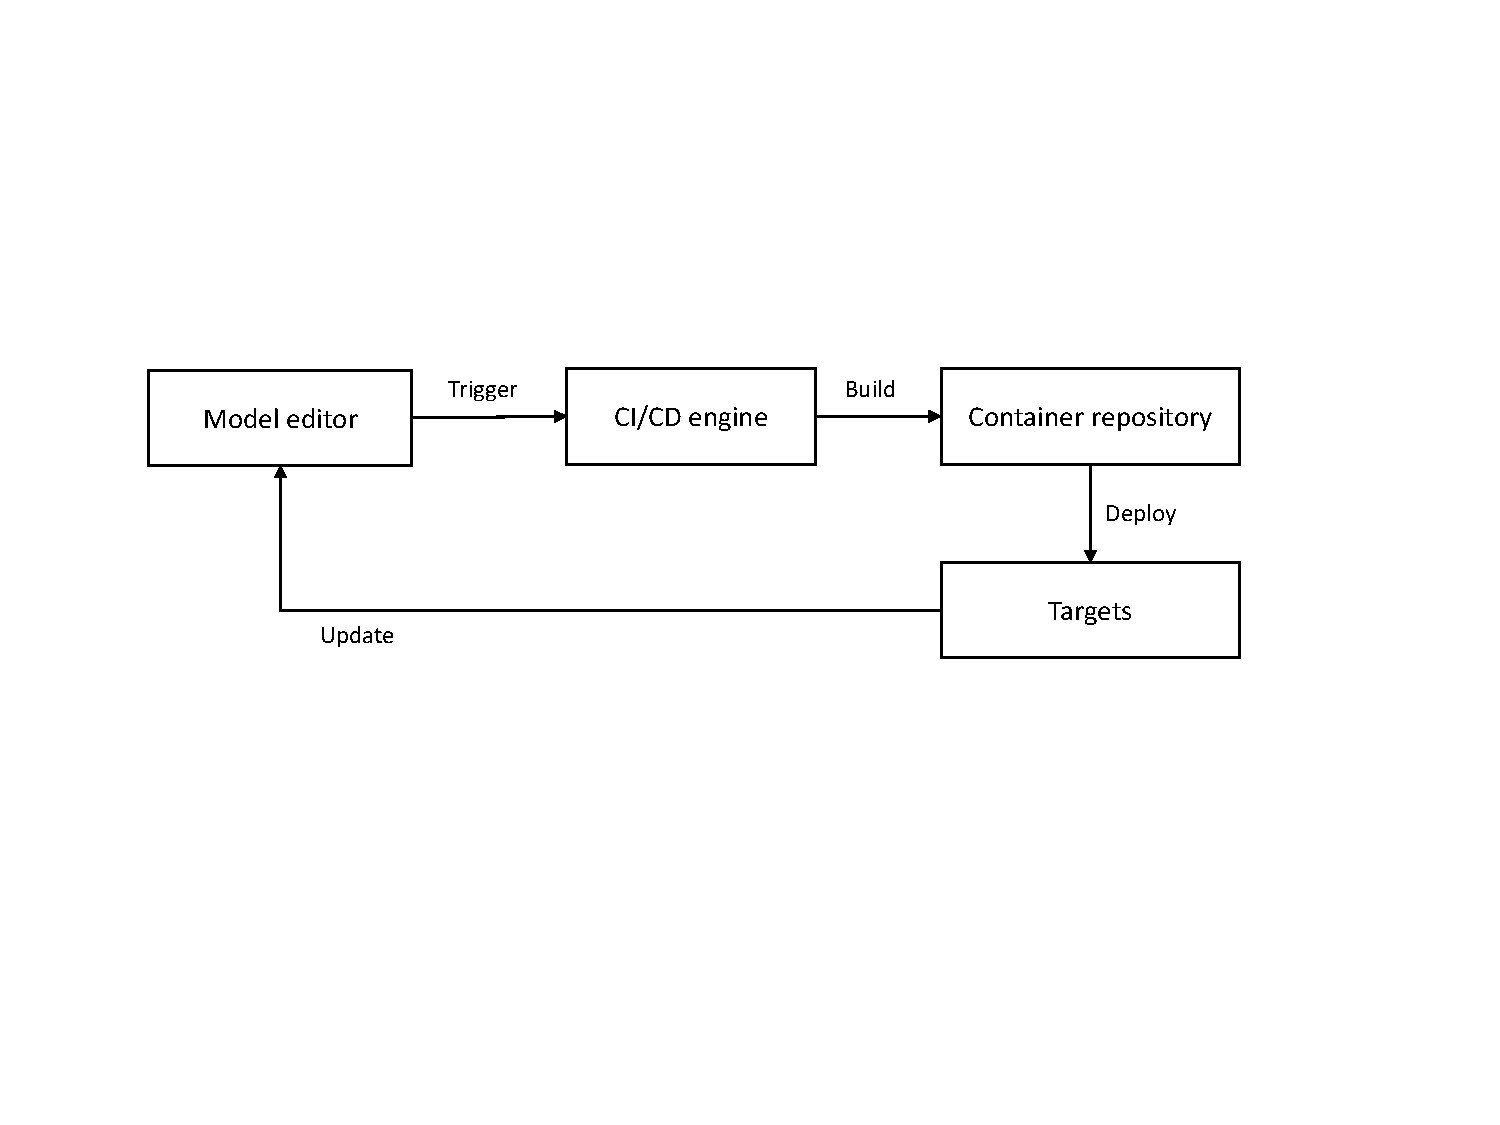
\includegraphics[scale=0.6]{figures/twinops_workflow.pdf}
  \caption{TwinOps workflow}
  \label{fig:twinops_workflow}
\end{figure}

\begin{itemize}

\item \textbf{Model editor}: responsible for building models, drawing the ports topology, and configuring the initial states. 
\item \textbf{CI/CD engine}: integrating the models committed by the previous pipeline stage; validating the models with real-world data; building the containerized image upon passing of all integration tests.
\item \textbf{Container repository}: a hub which stores numerous iterations of models' artifacts---such as the generated code---for the targets. This allows the targets to use the latest codes or rollback to previous versions. It is presumed that the targets in DTs run on diverse platforms (e.g., x86, x64, or ARM), hence the container infrastructure helps to distribute the artifacts efficiently.
\item \textbf{Targets}: a collection of PEs, which can pull the updated program from the repository, as well as produce data analytics which are used for the services.

\end{itemize}

It is important to recognize that the TwinOps framework is not bound to specific technologies or tools. The DT operator has the liberty to choose the collection of building blocks which fits best to the use case, as long as this choice is able to fulfill the workflow outlined in Figure \ref{fig:twinops_workflow}. The toolset implemented in the microbrewery DT will be described in Subsection \ref{sec:s1twop}.

\subsection{ThingsBoard} \label{sec:selframe_tb}
ThingsBoard \cite{Thingsboard} project supports M2M-style network. Essentially, it is an open-source platform that enables rapid development, management, and scaling of IoT projects. The key concepts of ThingsBoard are that the user can provision devices and assets; define relations between them and build rule chains that handle the event processing across the relations. From these features, we see the potentials in supporting the integration and orchestration of our DT. Figure \ref{fig:thingsboard_workflow} illustrates the workflow.

\begin{figure}[hbt!]
  \centering
  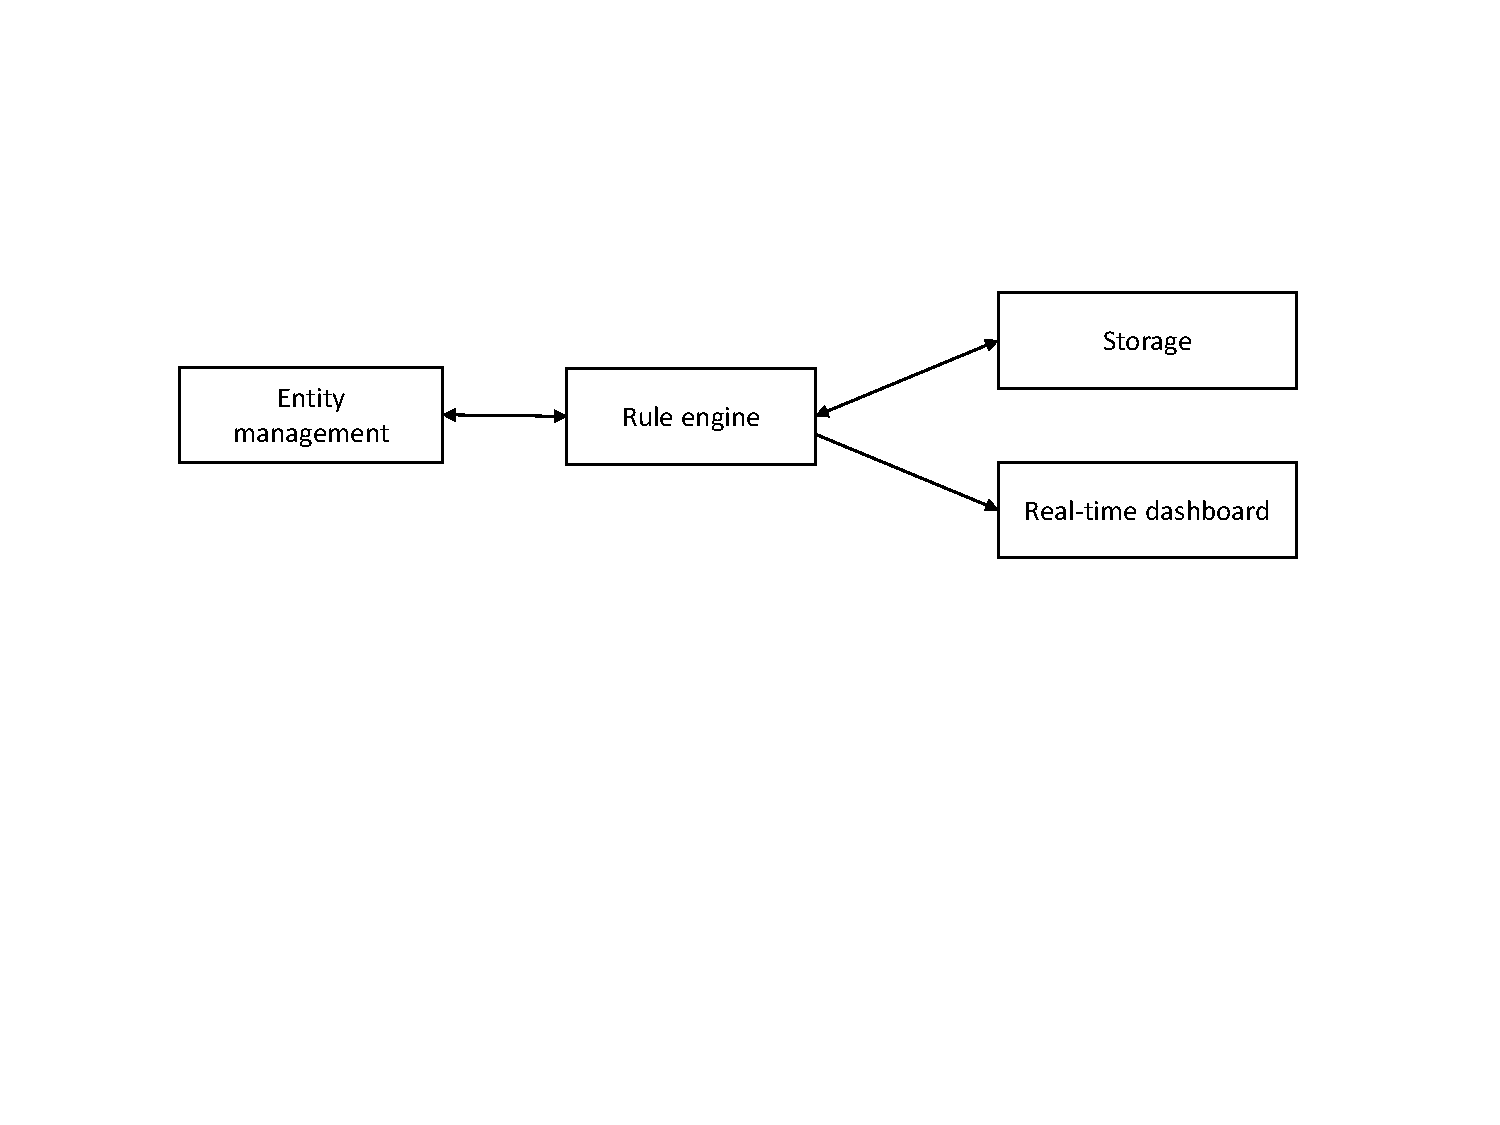
\includegraphics[scale=0.6]{figures/thingsboard_workflow.pdf}
  \caption[ThingsBoard workflow]{ThingsBoard workflow. The arrows represent the direction in which each stage could make modifications to the other stages}
  \label{fig:thingsboard_workflow}
\end{figure}

\begin{itemize}
\item \textbf{Entity management}: this is the first step where the user should define all the involved entities and their relations. There are two main entity types. \textit{Device} entity type refers to the basic unit that transmit and receive messages. The \textit{Asset} entity is an abstract type that can form logical grouping of \textit{devices} or other \textit{assets} via \textit{relations}. Commonly used \textit{relations} are ``contains", ``manages", etc.

\item \textbf{Rule engine}: refers to the event-based \textit{rule chains} which are customized by the user. A rule chain consists of connected \textit{rule nodes} which represent functions or conditions. There are built-in node type such as ``filter" or ``transform", etc. The user can also define their own nodes using JavaScript. When a message arrives from the entities the rule engine will produce the corresponding actions based on the \textit{rule chains} and the \textit{relations} which have been given in the entity management stage. As an example, a ``smart building" could impose crowd traffic monitoring using \textit{rule chains} to broadcast the readings of the passengers counter---a \textit{device}---in one elevator to all the other elevators which the building---\textit{an asset}---``contains".

\item \textbf{Storage}: ThingsBoard supports in-memory storage itself, or one can use the data the supported external space, e.g.,  cloud-based.

\item \textbf{Real-time dashboard}: this is related to the user experience and the user interface aspects. The operator can add \textit{widgets} in the dashboard to reflect the events happening in the rule engine in the forms of chart, table or various other visualizations.

\end{itemize}

There are a couple of underlying services called \textit{ThingsBoard Core} and  \textit{ThingsBoard Transports} that basically handle the M2M networking on the platform. They provide communication protocol stacks and account for maintaining the connectivity states. Consequently, they greatly influence system performance. Because these two are background processes, they are omitted in the workflow shown in Figure \ref{fig:thingsboard_workflow}.

\subsection{Ptolemy II}
In Subsection \ref{sec:orch} we have briefly described Ptolemy II from the perspective of actor-oriented model. Here we look at Ptolemy II from the software architecture angle. We aim to utilize it as a DT framework.

The official documentation \cite{Ptolemaeus2014} presents a meta model that describes the Ptolemy II software architecture, as seen in Figure \ref{fig:pt2meta}. Below are some important highlights of the figure:

\begin{itemize}
\item Every component in a Ptolemy II model is an instance of the \texttt{NamedObj} class. There are four subclasses of \texttt{NamedObj}. These are \texttt{Attribute}, \texttt{Entity}, \texttt{Port}, and \texttt{Relation} respectively.
\item \texttt{Relation} class represents communication path between the instances of \texttt{Entity}. 
\item \texttt{Port} class has many-to-many links to \texttt{Relation}, and it also hosts the \texttt{Receiver} interface that implements methods relating to data communication. Together they can be used to manage the models integration. 

\item Implemented by \texttt{Director}, the \texttt{Executable} interface contains methods that orchestrate the modeling progressions. In other words, the interface coordinates the iterations among actors based on the rules of the selected MoC.
\end{itemize}

\begin{figure}[hbt!]
  \centering
  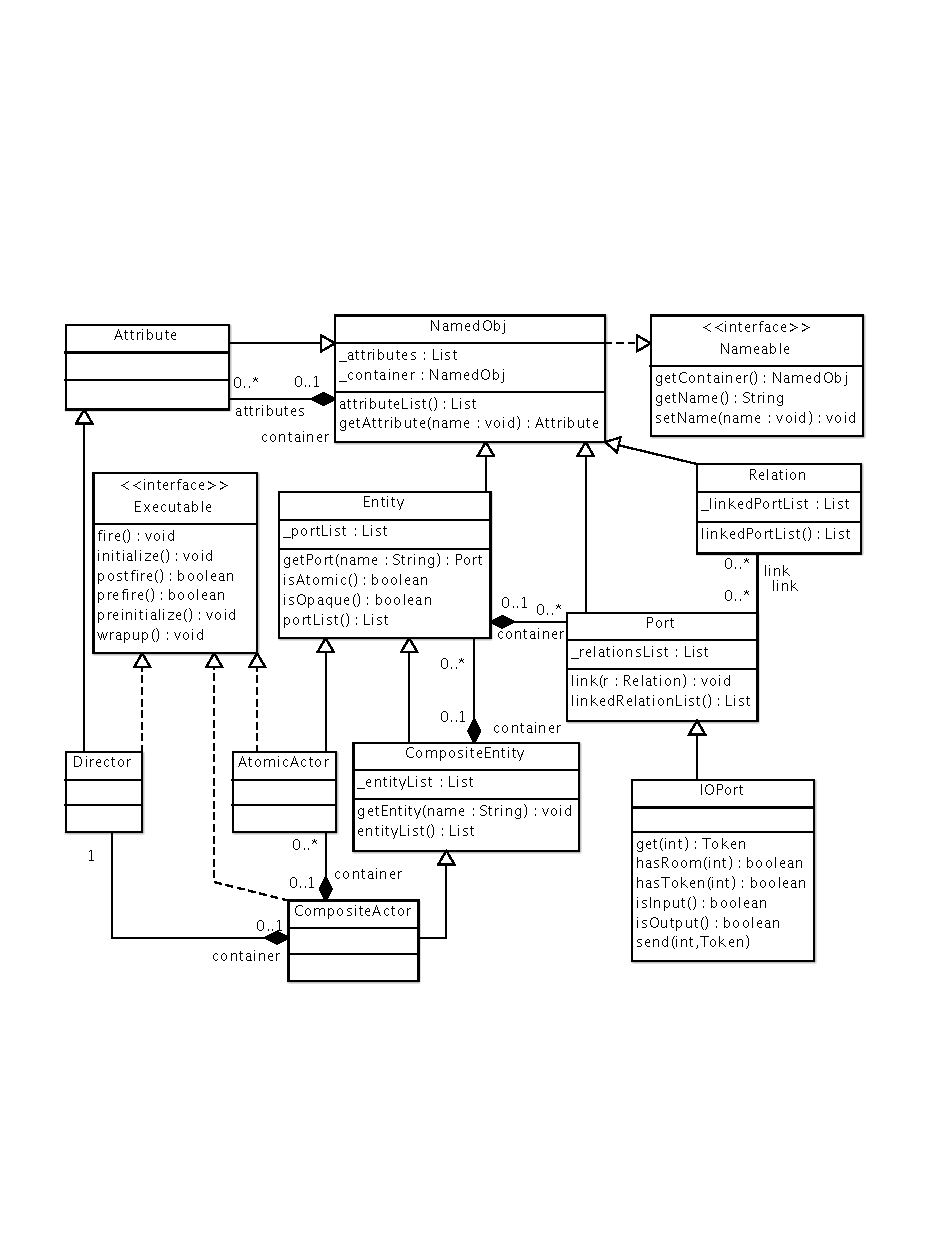
\includegraphics[scale=0.8]{figures/pt2meta.pdf}
  \caption{Meta model of Ptolemy II}
  \label{fig:pt2meta}
\end{figure}

The abstract syntax are implemented as a collection of Java classes and packages. Ptolemy II enables the user to interact with these abstract syntax by the mean of a graphical editing interface, utilizing drag-and-drop actions to accomplish designs.



\clearpage

\chapter{Implementation}\label{ch:implementation}
This chapter presents the implementations\footnote{This is an open source project. One can find the essential software implementations on our GitLab page at \url{https://gitlab.tue.nl/20181234/brewery_dt}, as well as the overview of equipment in Appendix \ref{apd:workbench}.} of \textbf{S1} (Production Prediction) and \textbf{S2} (Production Control) mentioned in Chapter \ref{ch:methodology}, using each of the three selected frameworks in order to showcase the possibilities of integration and orchestration approaches. As explained in Section \ref{sec:5dbrewery}, \textbf{S3} and \textbf{S4} are not implemented in this project.

Despite the influence of bio-chemistry theme in our case study, we choose to convert all VE models to FMUs over the CAPE-OPEN standard for the sake of generalizing the approach so they can extend to other domains. As FMI is more inclusive to a wider range of models for integration.

\section{Production Prediction (S1) demonstrations}\label{sec:s1demo}
In \textbf{S1}, the DT collects readings from the three sensor devices of the PE. The scanning period is set to five minutes; we consider this frequency adequate for monitoring the slow variations of the process. After merging the monitoring data, the models of the VE will be invoked to compute the final predicted wort temperature using the given data. Besides, the three chemistry models (see also Section \ref{sec:5dbrewery}) have data dependency to one another.

\subsection{S1 in TwinOps} \label{sec:s1twop}
Figure \ref{fig:s1_twop_workflow} shows the technologies that compose the building blocks of the TwinOps workflow:

\begin{figure}[hbt!]
  \centering
  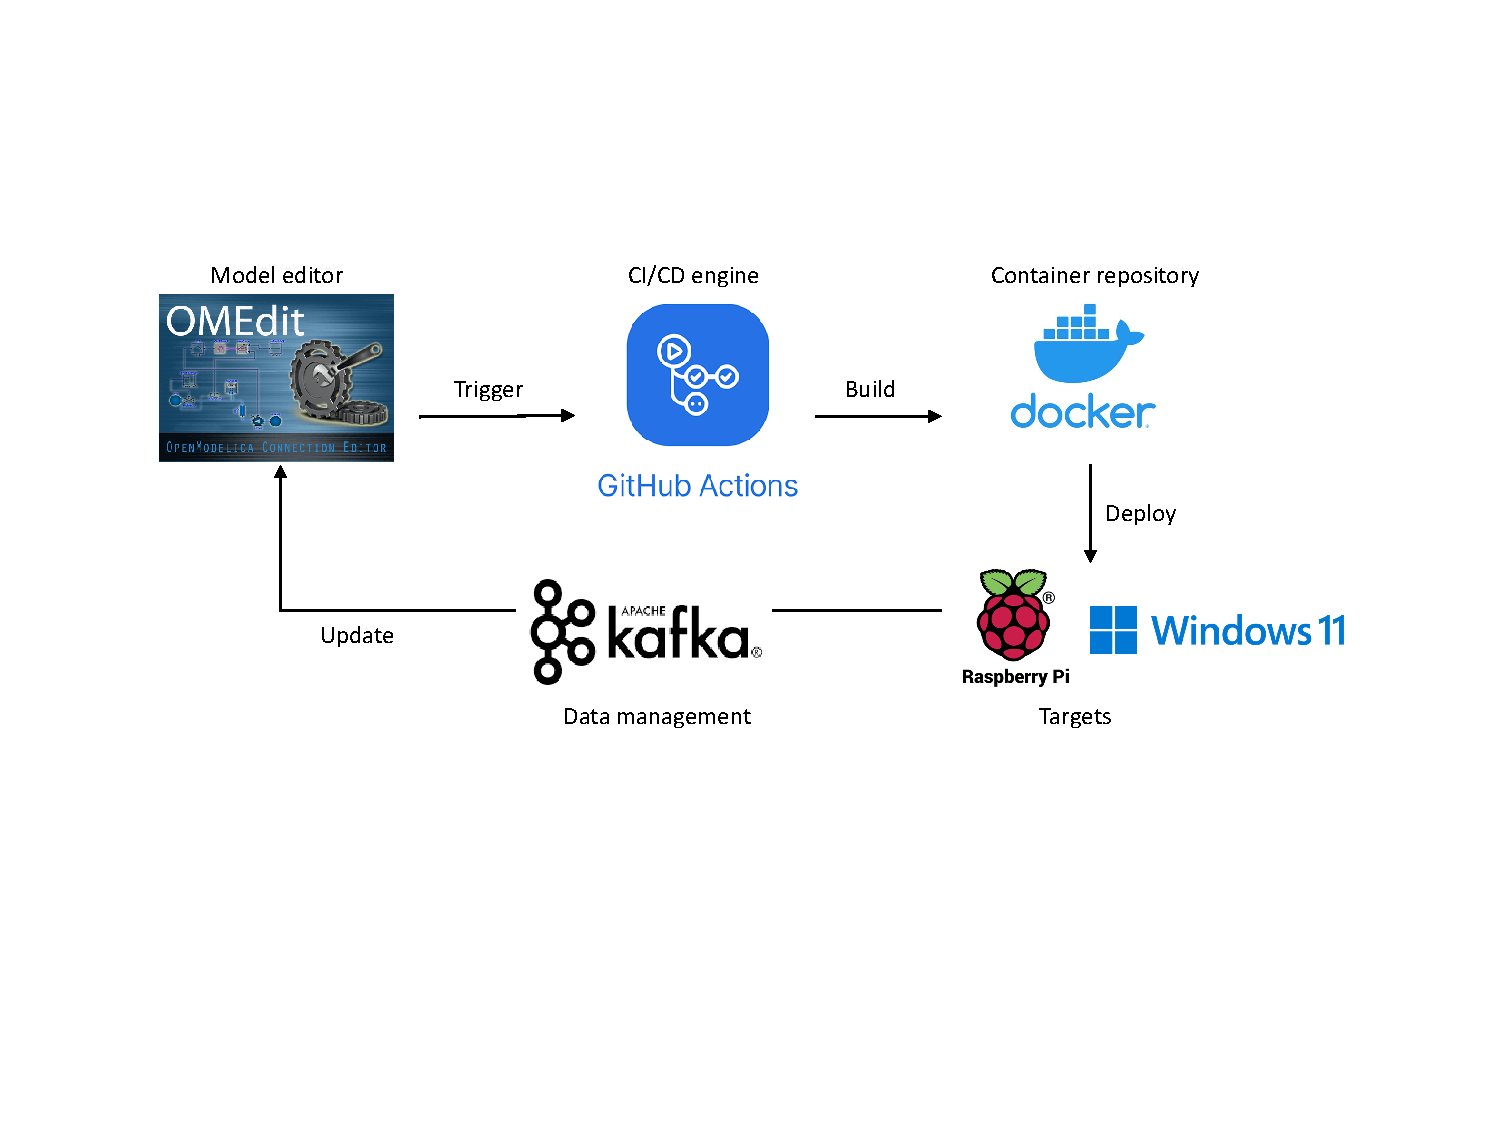
\includegraphics[scale=0.6]{figures/s1_twop_workflow.pdf}
  \caption{TwinOps implementation workflow for S1}
  \label{fig:s1_twop_workflow}
\end{figure}

For the \textit{model editor} stage, OMEdit \cite{OMEdit} is chosen to achieve the task. It is a graphical editing tool that allows user to connect individual FMUs to each other, and then export the topology to the System Structure and Parameterization (SSP) format \cite{SSP}. SSP is an open standard used to describe the port connections of a set of FMUs. It was created by the same organization which initiated the FMI standard, the Modelica Association. It is supported by an increasing number of major simulation environments which also support FMI. Figure \ref{fig:s1_twop_omedit} shows the layout of our use case in OMEdit.

\begin{figure}[hbt!]
  \centering
  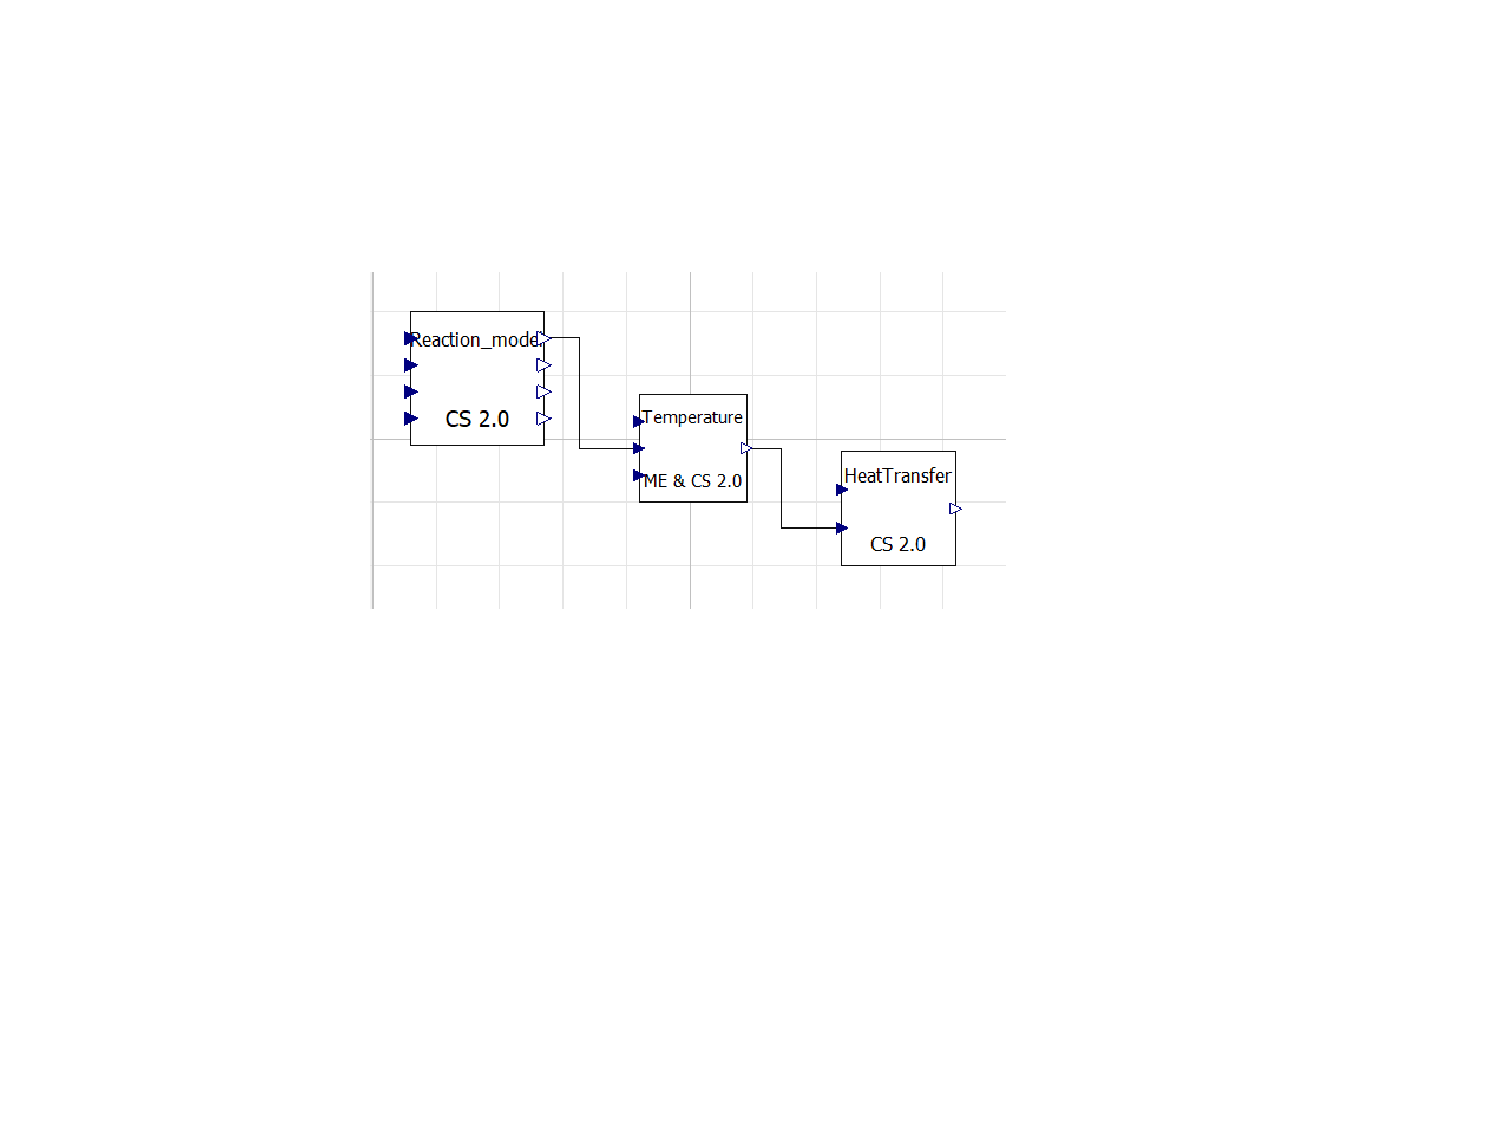
\includegraphics[scale=0.6]{figures/s1_twop_omedit.pdf}
  \caption[The SSP file rendered in OMEdit]{The SSP file rendered in OMEdit. Due to their different sources of origin, each FMU has varying supports for simulation modes, such as co-simulation version 2.0 (CS 2.0) or model exchange (ME). The FMUs also have different numbers of I/O ports. Since the models are designed to be``future-proof" for subsequent services, this is the reason why many I/O ports appear unused as they are irrelevant to this specific service}
  \label{fig:s1_twop_omedit}
\end{figure}

We choose GitHub Actions \cite{GitHubActions} as our \textit{CI/CD engine} for its native support for a vast variety of operating systems and programming frameworks. The operator can configure the pipeline using YAML---a human-readable data-serialization language that is commonly used for writing configuration files. 

As shown in Figure \ref{fig:s1_twop_cicd}, two phases (referred as jobs) are created in the pipeline, the left job represents CI, and the right job represents CD which will only be invoked if the CI job has succeeded. In the CI job, the SSP file is validated with the monitoring data which has been retrieved from a user-created trigger which activates every time new data are detected. The results will be saved as a GitHub Actions artifact. In the CD job, the task is to build and push the container image in Docker format \cite{Docker}.

\begin{figure}[hbt!]
  \centering
  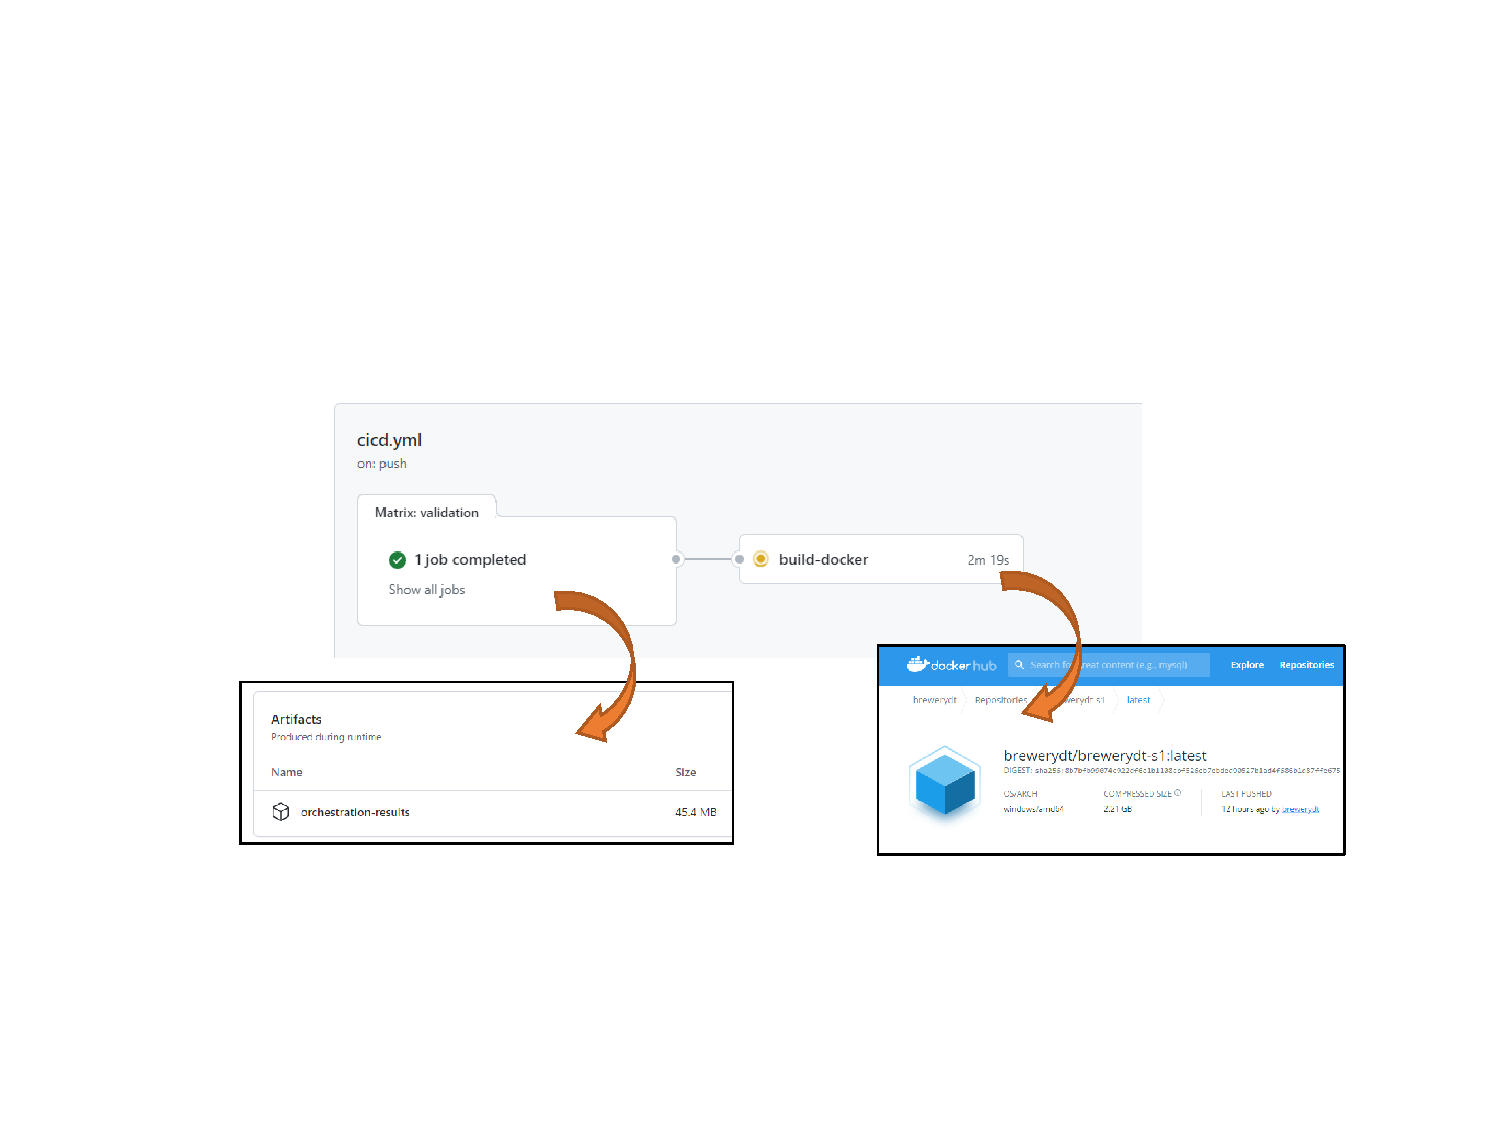
\includegraphics[scale=0.65]{figures/s1_twop_cicd.pdf}
  \caption{The CI (left) and CD (right) jobs and their outputs}
  \label{fig:s1_twop_cicd}
\end{figure}

The \textit{targets} for our use case are Raspberry Pi and Windows PC. The former is used as a data aggregation hub for all the sensor controls, and the latter is where we host our VE models.

One might notice the Kafka \cite{Kafka} block was not originally present in Subsection \ref{sec:selframe_twop} as a workflow stage. The reason being, the update path from the \textit{targets} to the \textit{model editor} stage could range from simplistic to rather complex, depending on the actual building blocks applied. In our use case, the \textit{targets} involve two different platforms---a microprocessor and a PC, leading us to introduce Kafka as an auxiliary tool to simplify the data management. In the DT context, models may access and store data in different formats and frequency. We adopt Kafka over the more traditional database due to its advantages of compartmentalized data queue and its active data streaming API. One can read more about the principles of Kafka in Appendix \ref{apd:kafka}.

\subsection{S1 in ThingsBoard}
Figure \ref{fig:s1_tb_entity} shows all the \textit{device} entities (sensors) and the \textit{asset} entities used in \textbf{S1}. The entities can be added by the operator manually in ThingsBoard UI, or be provisioned in bulk using CSV file. If multiple devices share the common settings, then one might consider creating ``device profiles" to improve entity management, like the ``Sensors" profile or the ``Models" profile shown in the figure. 

The asset named ``DT-PE" has a ``contain" \textit{relation} to all devices of the ``Sensors" profile. In other words, ``DT-PE" is an amalgamation of devices of the sensor type. The \textit{relation} defines a namespace which the \textit{rule chain} will adhere to.

\begin{figure}[hbt!]
  \centering
  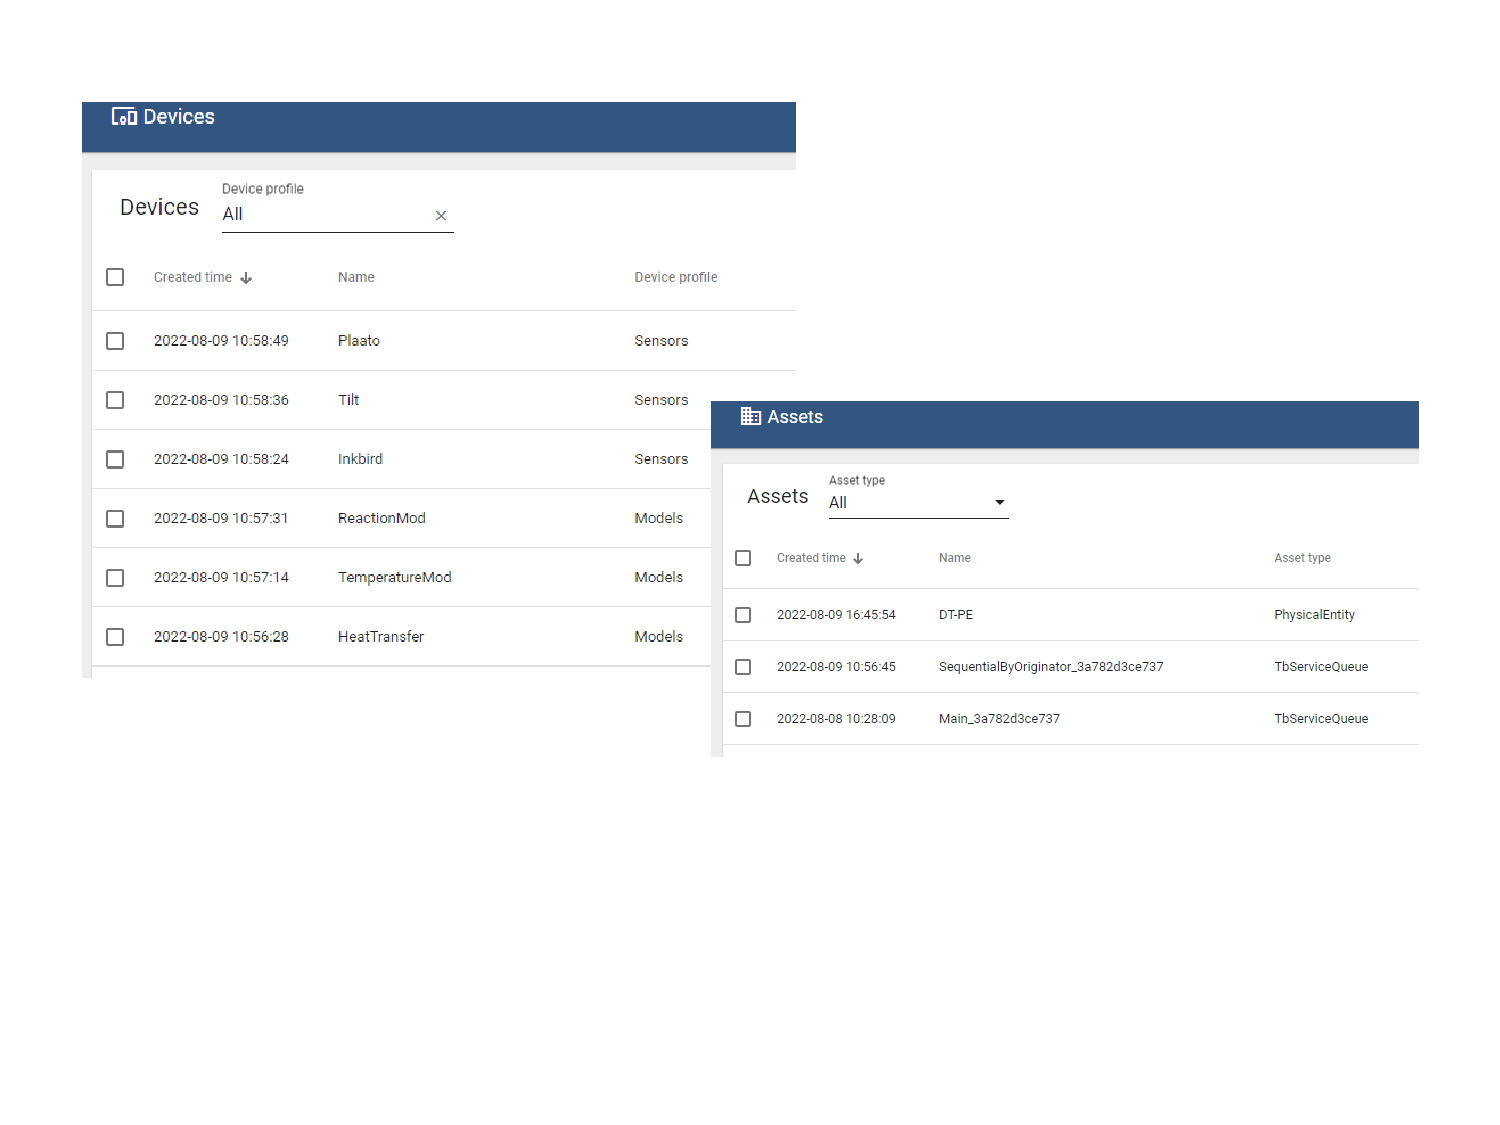
\includegraphics[scale=0.6]{figures/s1_tb_entity.pdf}
  \caption[S1 entity management in ThingsBoard]{S1 entity management in ThingsBoard. \texttt{Plaato} is the sensor used for collecting multitude of fermenter statuses; \texttt{Tilt} is a gravity detector; \texttt{Inkbird} is an ambient thermostat. The asset type \texttt{TbServiceQueue} is auto-generated  by the core process to handle network traffics.}
  \label{fig:s1_tb_entity}
\end{figure}

\begin{figure}[hbt!]
  \centering
  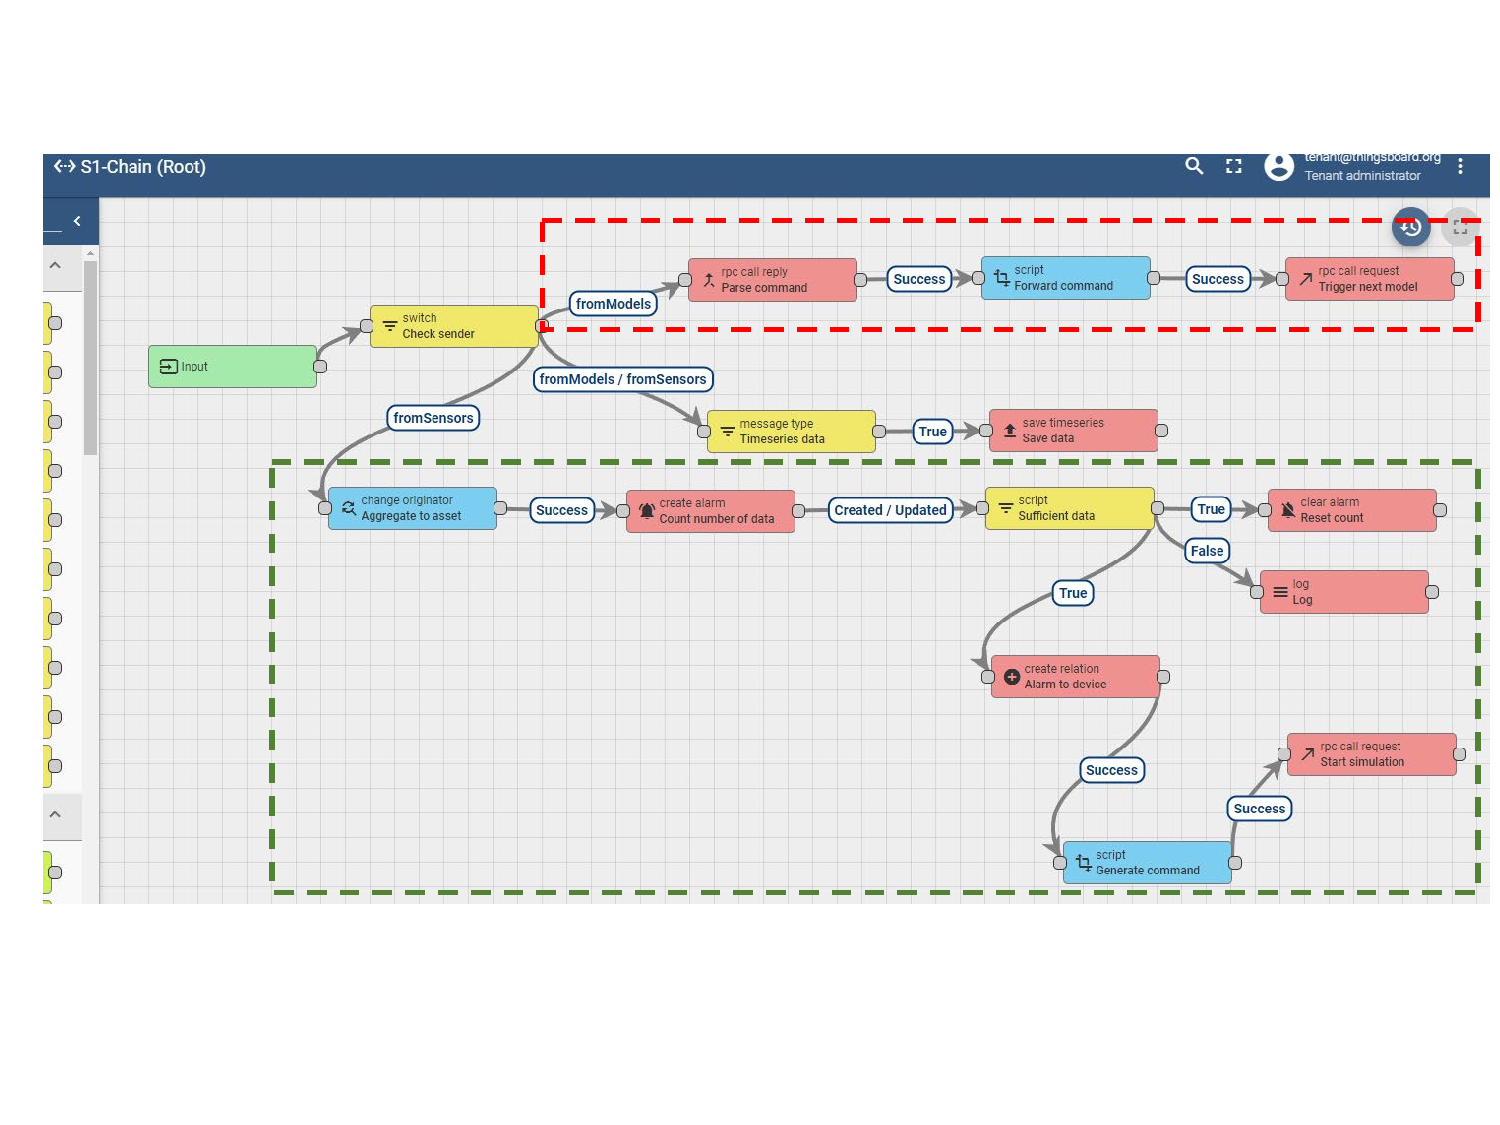
\includegraphics[scale=0.6]{figures/s1_tb_rulechain.pdf}
  \caption{S1 rule chain in ThingsbBoard}
  \label{fig:s1_tb_rulechain}
\end{figure}

Figure \ref{fig:s1_tb_rulechain} presents the \textit{rule chain}, which has three major parts:
\begin{itemize}
\item The top branch (red dashed border) is the event-based logic for inter-models procedure calls. Its primary function is to orchestrate by signaling from the originator model to the destination model, such that a correct execution sequence could be maintained. 
\item The bottom branch (green dashed border) is for updating the monitoring data from the sensors to the model states. The ``DT-PE" asset plays an important role here for transforming the local namespace of the sensor data into the global namespace of the DT, such that the models can use the data without binding to specific sensor devices.
\item The nodes in the middle are responsible for recording and saving data with timestamps for future usage by the real-time dashboard. 
\end{itemize}

\begin{figure}[hbt!]
  \centering
  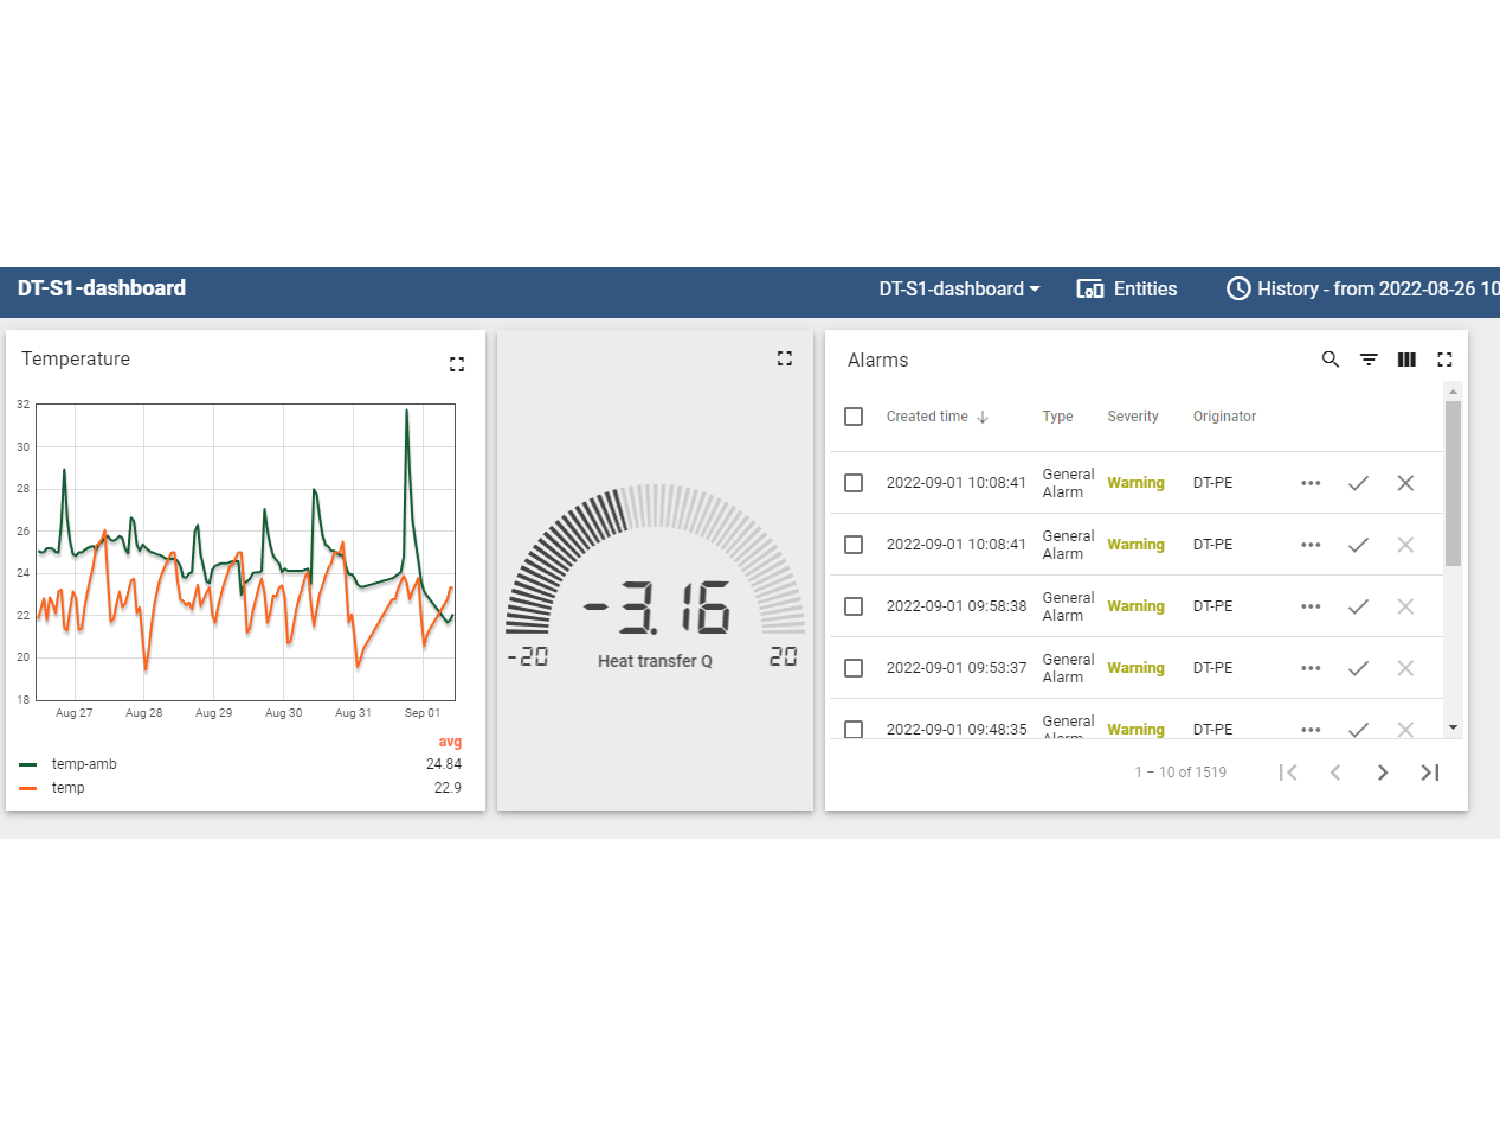
\includegraphics[scale=0.5]{figures/s1_tb_dashboard.pdf}
  \caption{A snapshot of the real-time dashboard in ThingsBoard for the \textit{heat transfer model}}
  \label{fig:s1_tb_dashboard}
\end{figure}

As introduced in Subsection \ref{sec:selframe_tb}, the real-time dashboard offers a wide range of \textit{widgets} for the operator to incorporate the human-in-the-loop concept to DT operations. In Figure \ref{fig:s1_tb_dashboard} we demonstrate the usage of built-in \textit{widgets} that visualize the system information. The plot on the left records the temperatures monitored from the PEs. The middle gauge displays the heat loss prediction at a given future moment. The alarm widget on the right side notifies the operator every time the \textit{heat transfer model} has been updated.

\subsection{S1 in Ptolemy II} \label{sec:s1demopt2}

\begin{figure}[hbt!]
  \centering
  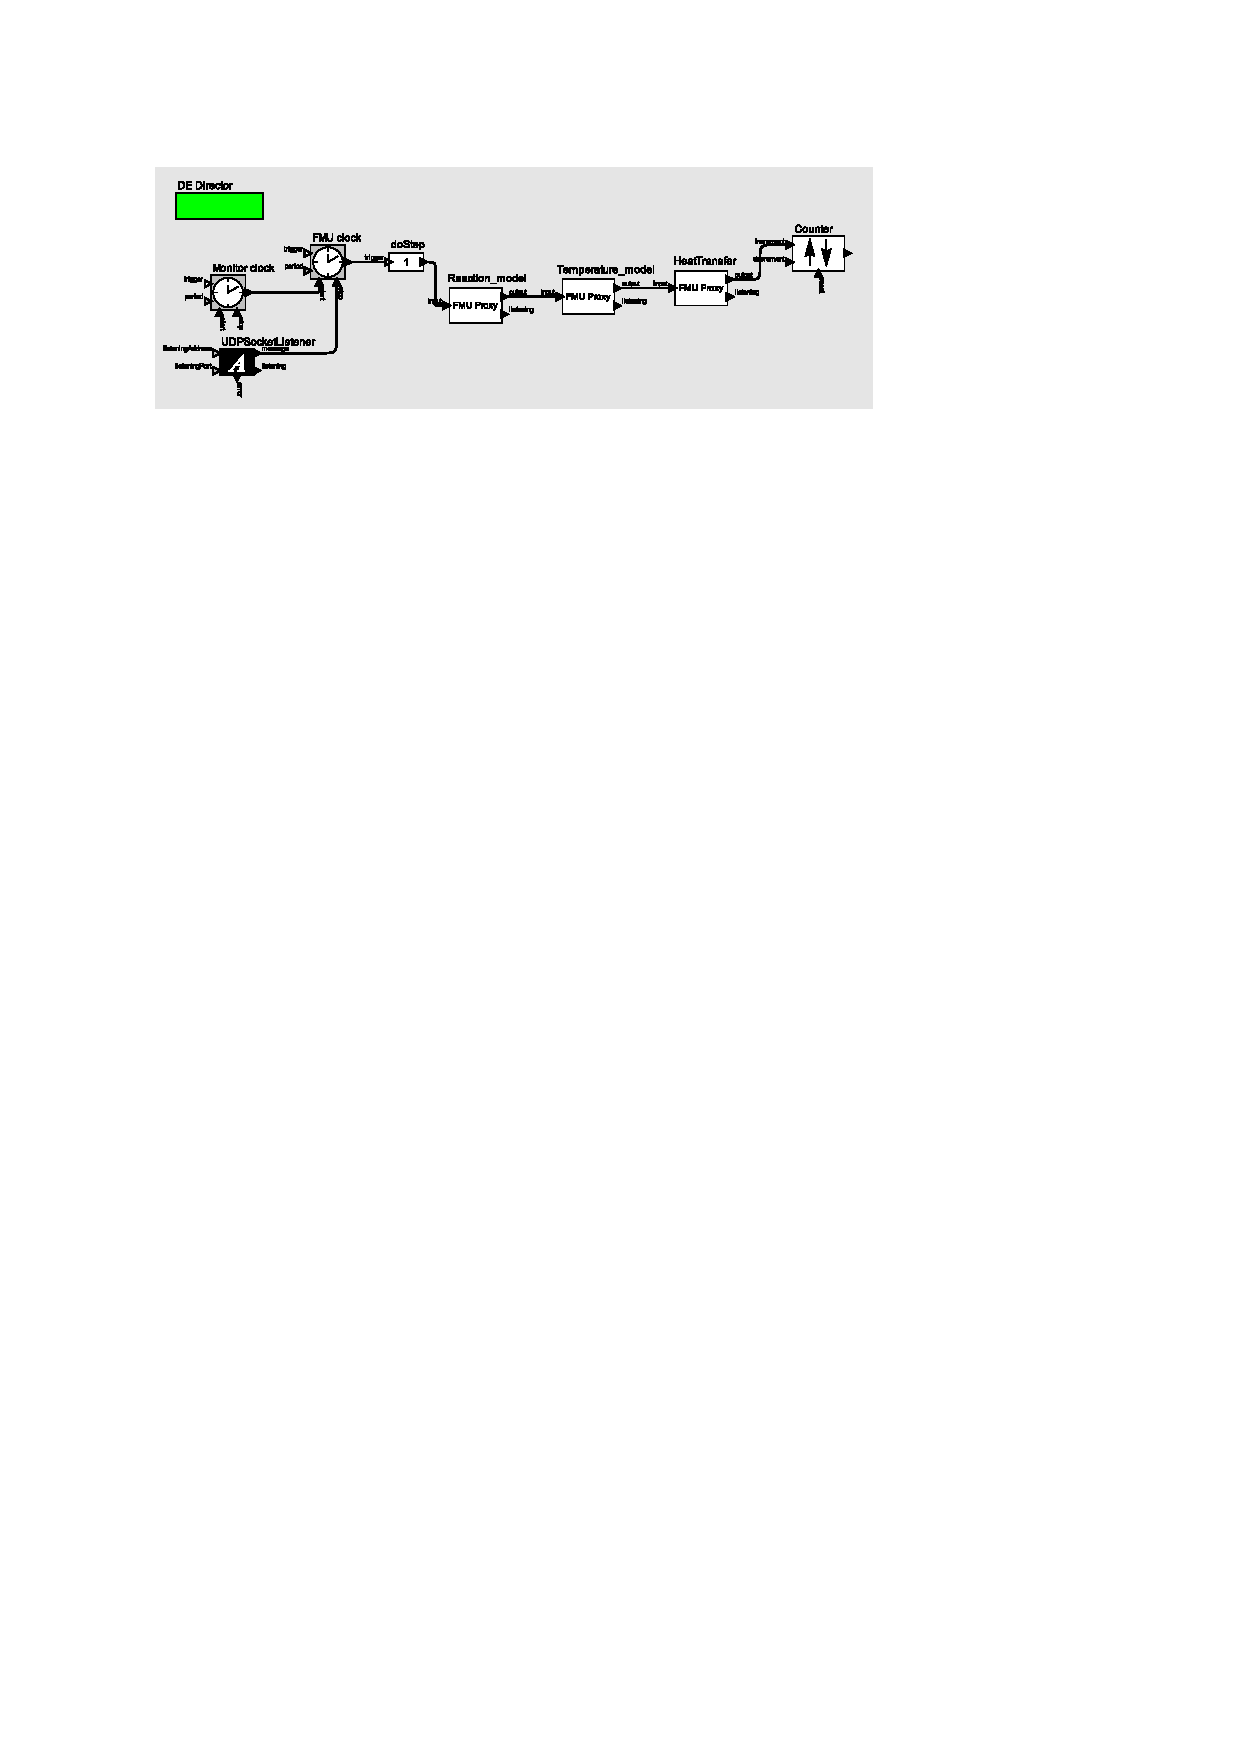
\includegraphics[scale=1.1]{figures/s1_pt_de.pdf}
  \caption{Ptolemy II design for S1}
  \label{fig:s1_pt_de}
\end{figure}

Figure \ref{fig:s1_pt_de} displays the overall design of \textbf{S1}. The Discrete Event (DE) \texttt{Director} is used as the orchestrating instructions are treated as individual ``events". There are two clock sources, \texttt{Monitor clock} is synchronized against real-world time such that it takes up the task to trigger the models based on the sensor events of PEs. On the other hand, \texttt{FMU clock} dictates the time advancement of the FMU models. It is initialized---by \texttt{Monitor clock}---when the monitoring data are ready, and is terminated when all models have completed simulations---notified via a dedicated UDP listener. Each \texttt{FMU Proxy} represents a model of the VEs.

Since Ptolemy II does not posses data management actors suitable for our DT, we utilize Kafka to fetch the monitoring data in order to update the models and to store the computed results.

Although Ptolemy II has built-in support for FMI by its \texttt{FMUImporter} actor, however, from our experiments we discover it has several weaknesses which lead to undesirable crashes (see Appendix \ref{apd:fmi} for details). As a circumvention, a user defined actor named \texttt{FMU Proxy} is created as shown in Figure \ref{fig:s1_pt_proxy}. The actor serves as a middle-man who forwards the orchestrating instructions from Ptolemy II to the solver outside of the environment via UDP sockets. Using this approach, the operator can orchestrate the FMU models as if they are inside the Ptolemy II environment.   

\begin{figure}[hbt!]
  \centering
  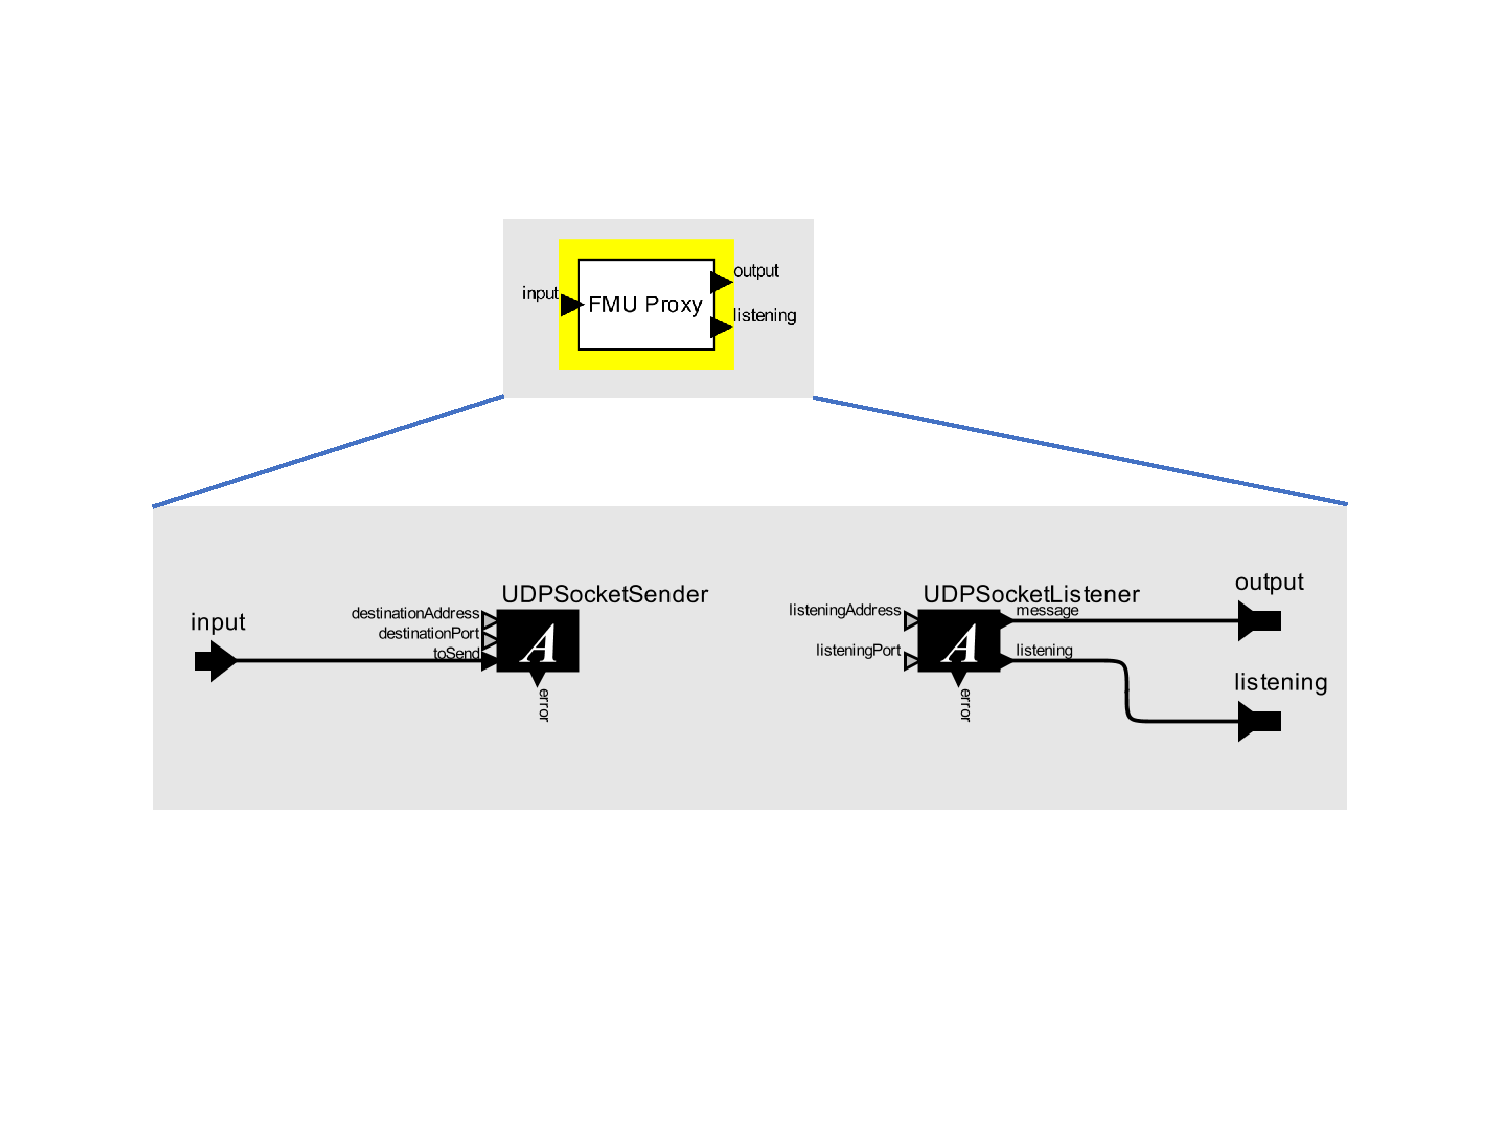
\includegraphics[scale=0.45]{figures/s1_pt_proxy.pdf}
  \caption{The internal implementation of \texttt{FMU Proxy}}
  \label{fig:s1_pt_proxy}
\end{figure}

\section{Production Control (S2) demonstrations}\label{sec:s2demo}
In \textbf{S2}, the control model generates a command based on the fed data. Then the commands are sent from the VE to the actuator---a water pump controller---of the PE. Most of the framework infrastructures are inherited from \textbf{S1}. As more services are introduced, we start to benefit from the dividends of frameworks in term of a significant reduction in developer's workload. 

An alternative implementation that uses human-in-the-loop control scheme instead of fully automated decisions can be found in Appendix \ref{apd:humanloop}. The alternative demonstrates how DTs can be used to assist the operators in a scenario where human intervention is necessary.  
  
\subsection{S2 in TwinOps} 
On top of the existing \textbf{S1} workflow, the operator can simply add the new model to the SSP file as in Figure \ref{fig:s2_twop_omedit}. After that, a new task needs to be added to the CI/CD pipeline so as to pass the computed commands to a remote webhook that controls the water pump.

\begin{figure}[hbt!]
  \centering
  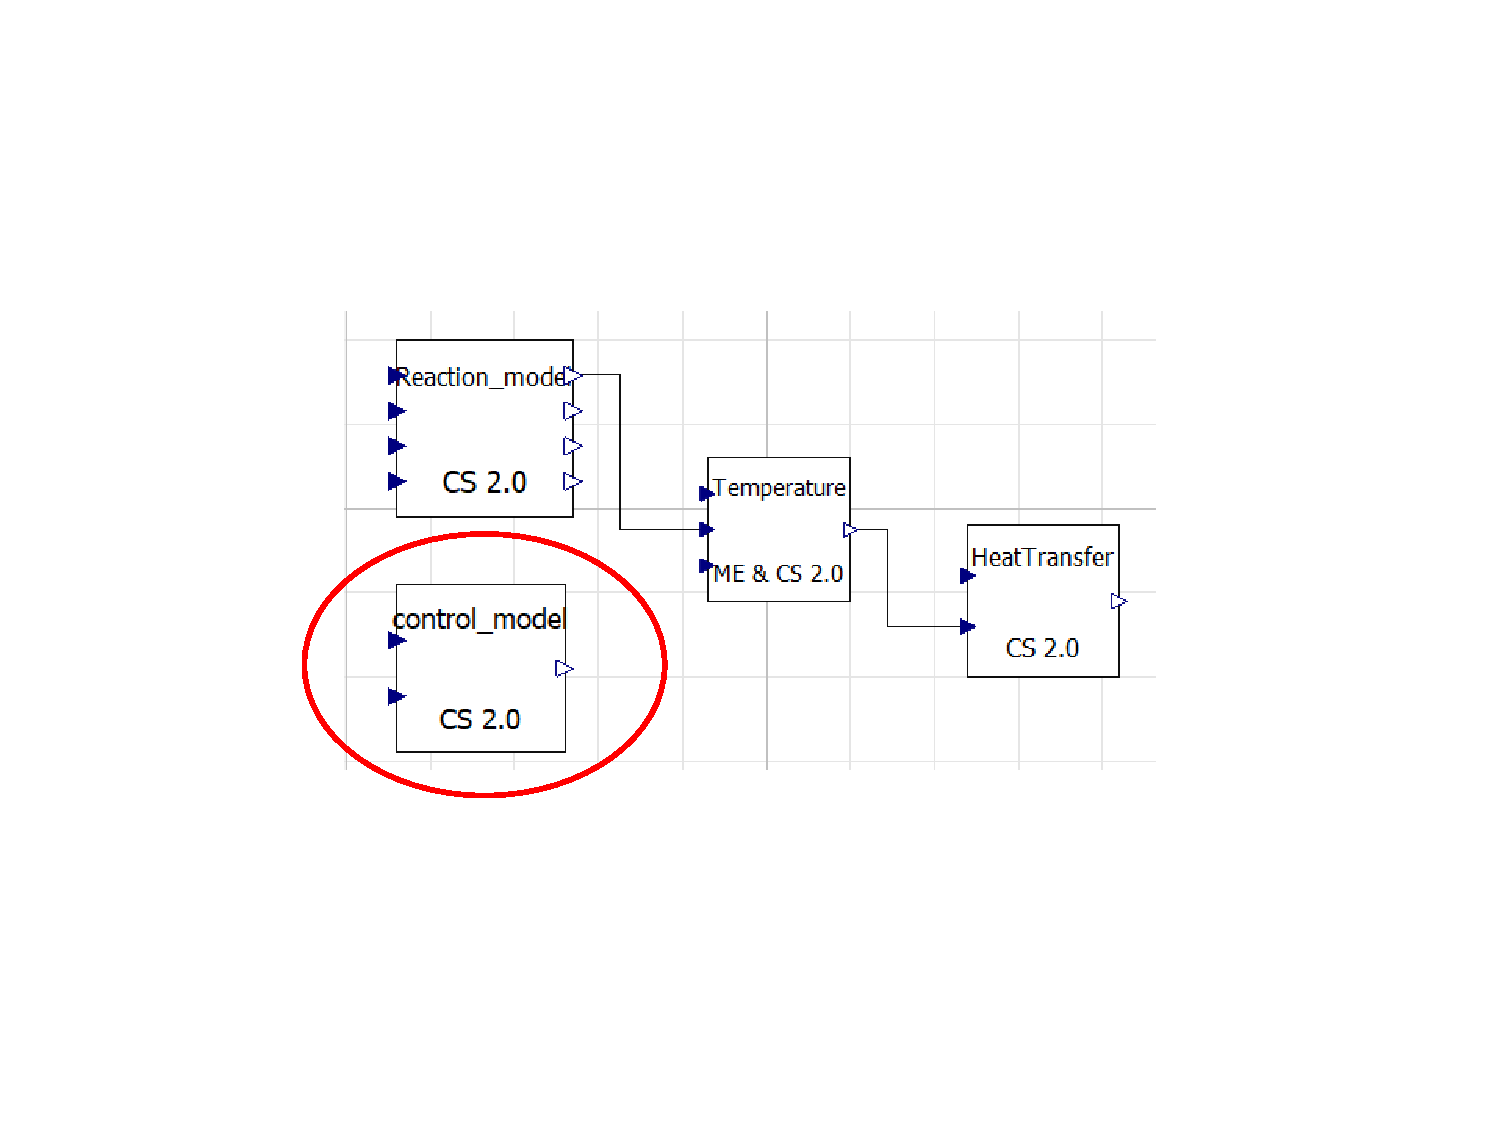
\includegraphics[scale=0.4]{figures/s2_twop_omedit.pdf}
  \caption{The SSP layout of S2}
  \label{fig:s2_twop_omedit}
\end{figure}

\subsection{S2 in ThingsBoard} 
The control model is provisioned as an entity of the ``Models" type just as with the models in \textbf{S1} previously.

A new \textit{rule chain} shown in Figure \ref{fig:s2_tb_rulechain} is added to support the control service. The top branch is responsible for triggering the control model, similarly to the way of \textbf{S1}. The bottom branch takes care of sending the command message to the actuator. 

\begin{figure}[hbt!]
  \centering
  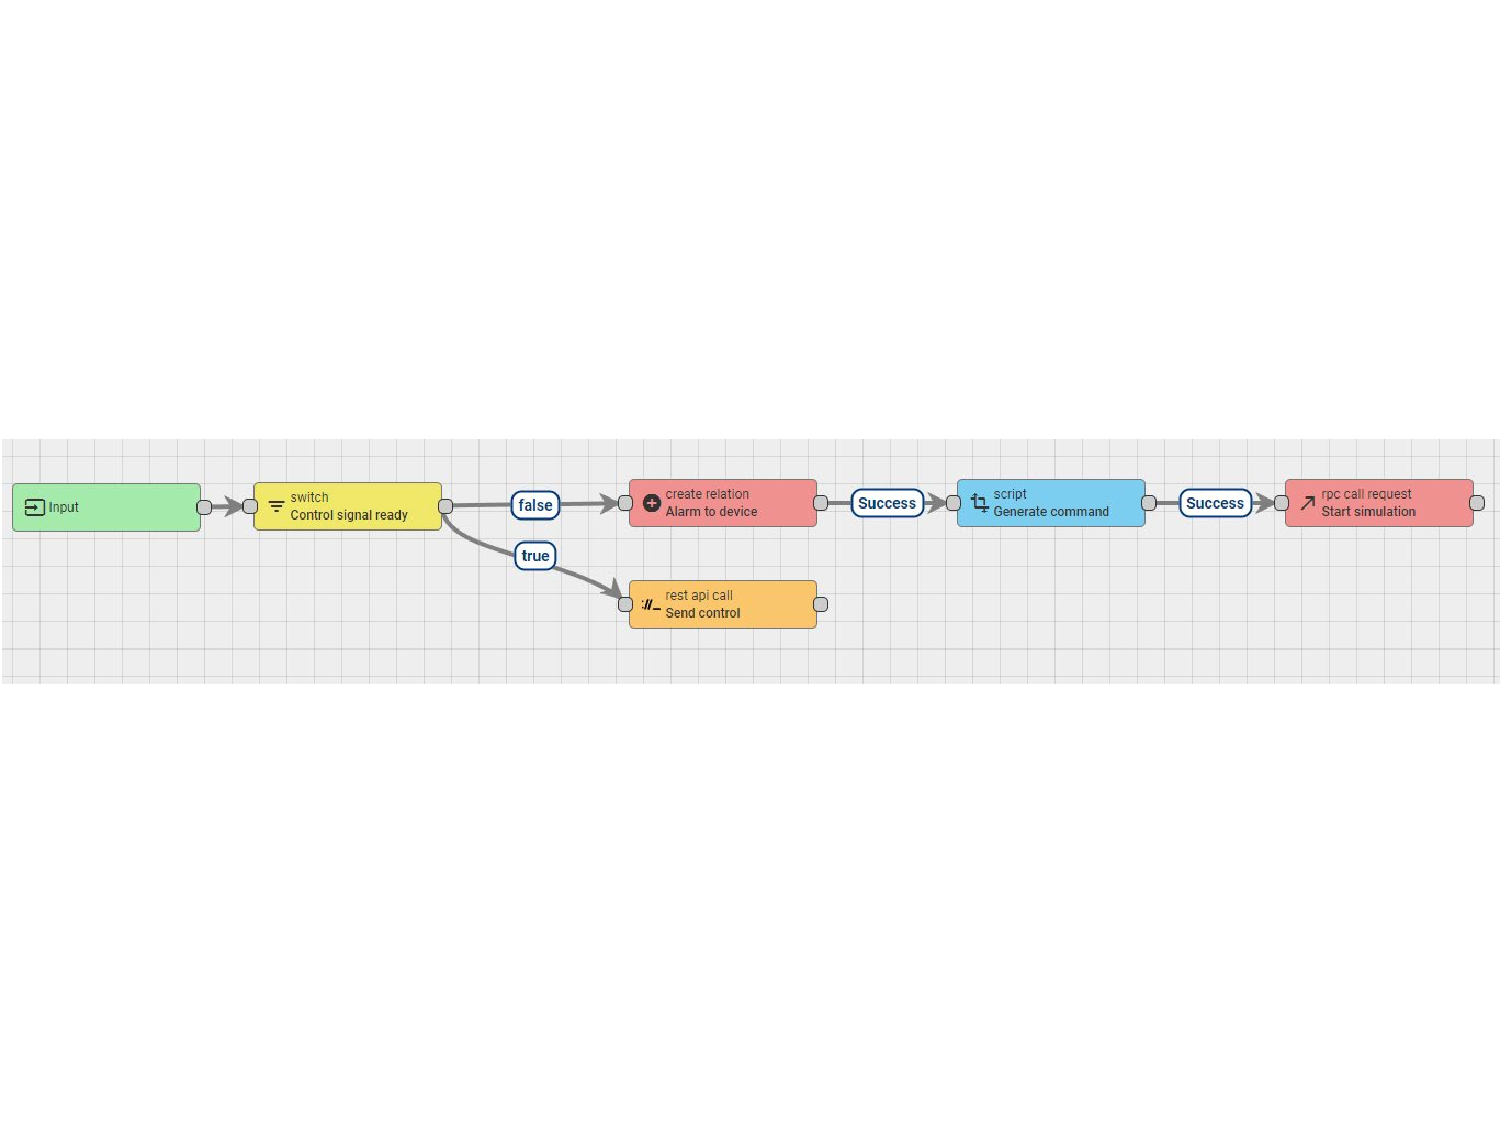
\includegraphics[scale=0.55]{figures/s2_tb_rulechain.pdf}
  \caption{S2 rule chain in ThingsBoard}
  \label{fig:s2_tb_rulechain}
\end{figure}

The \textbf{S2} \textit{rule chain} is connected to the ``root" \textit{rule chain} of \textbf{S1} via the ``Flow" type nodes (the purple color nodes in Figure \ref{fig:s2_tb_rulechain_root}), so the established data routing paths could be reused.

\begin{figure}[hbt!]
  \centering
  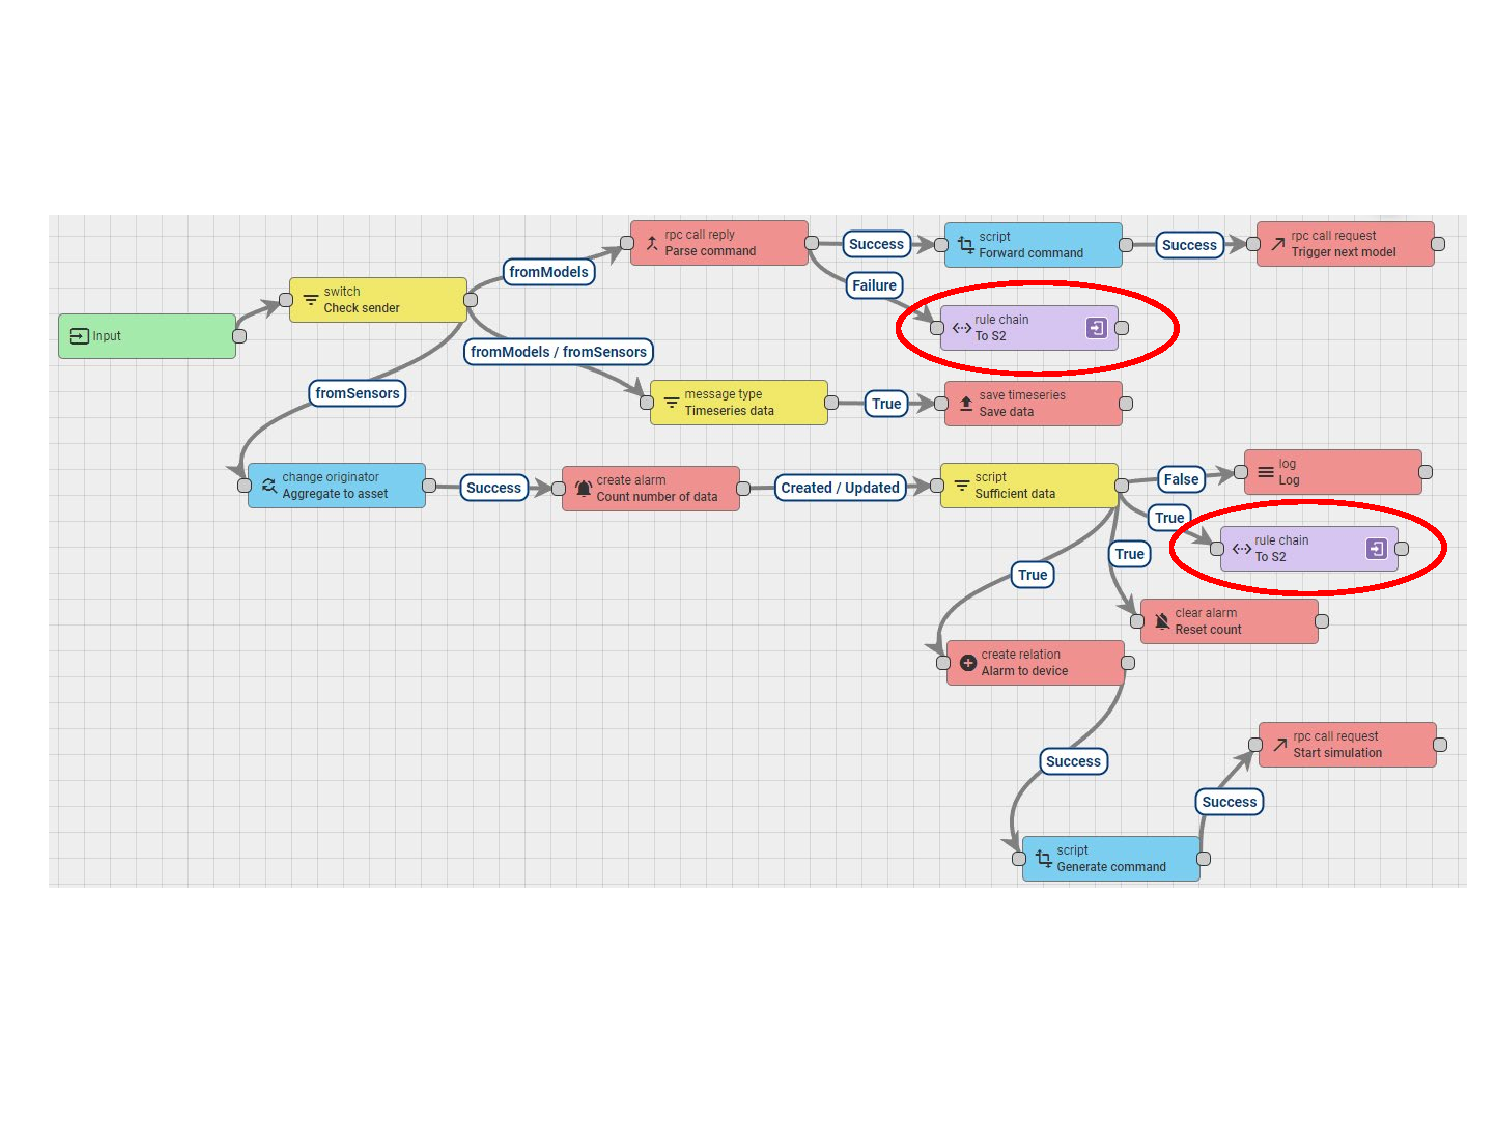
\includegraphics[scale=0.5]{figures/s2_tb_rulechain_root.pdf}
  \caption{Integration of S2 to the root rule chain}
  \label{fig:s2_tb_rulechain_root}
\end{figure}

In the real-time dashboard, the computed control signal are superimposed onto the timeseries chart of the temperatures, as shown in Figure \ref{fig:s2_tb_dashboard}. 

\begin{figure}[!htb]
  \centering
  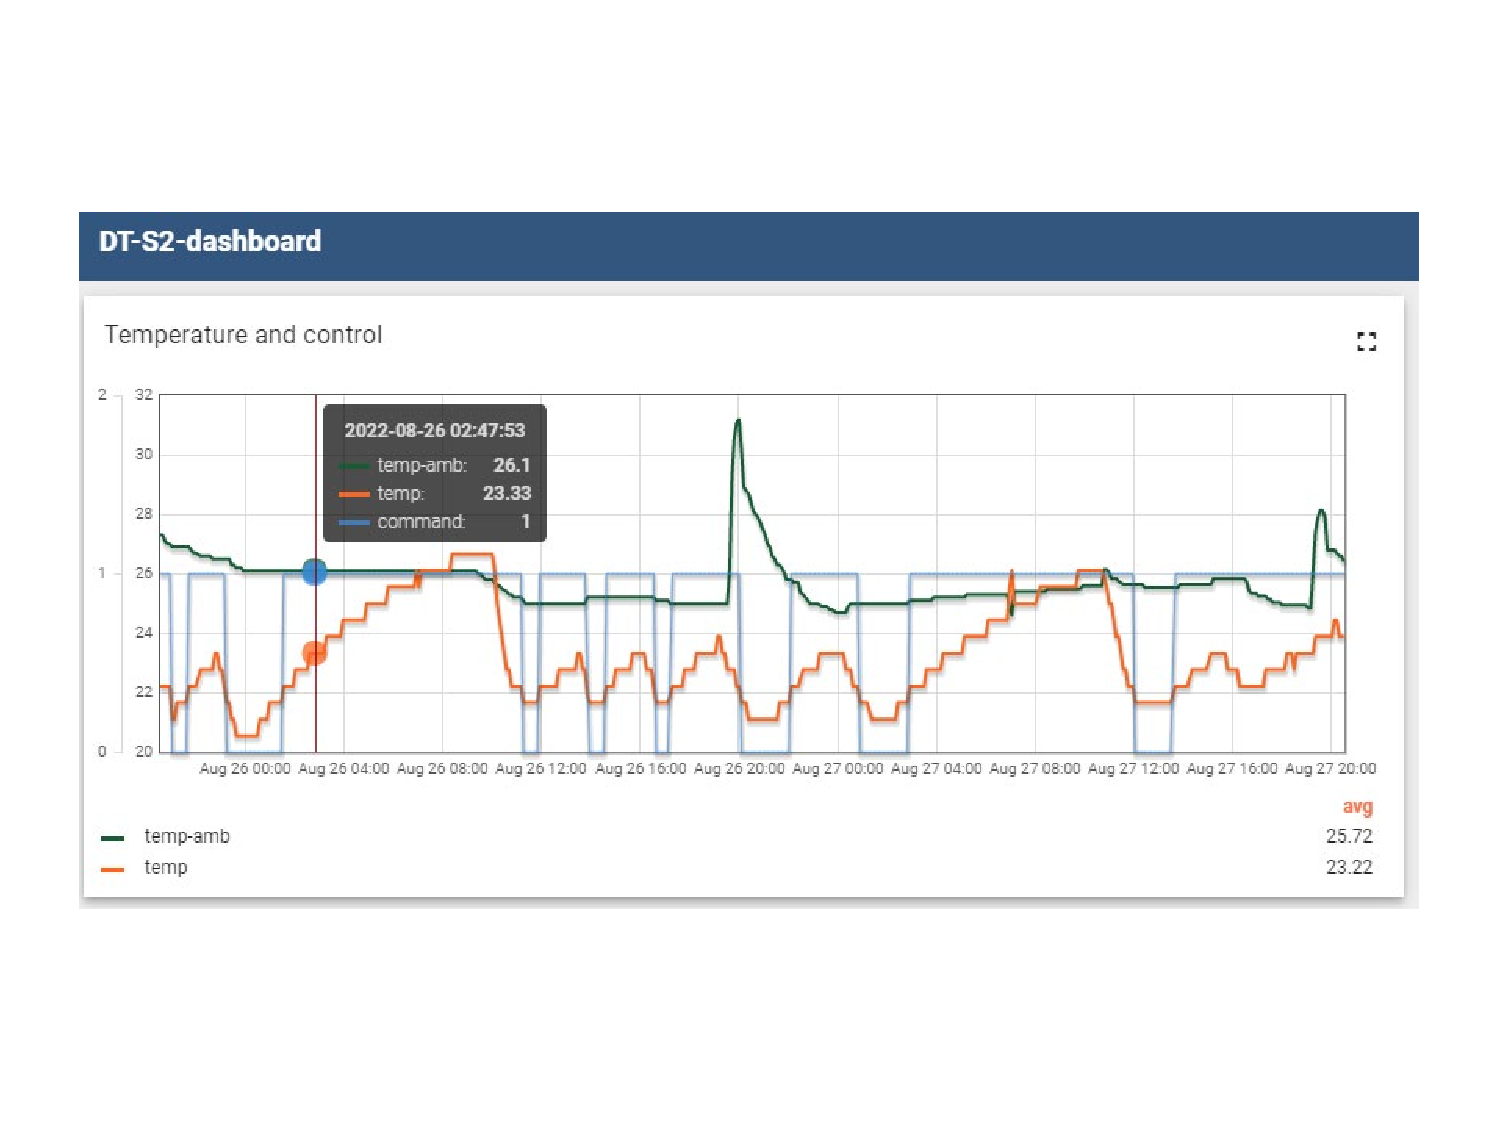
\includegraphics[scale=0.44]{figures/s2_tb_dashboard.pdf}
  \caption[A snapshot of S2 real-time dashboard]{A snapshot of S2 real-time dashboard. The chart displays the room temperature (green), the fermenter temperature (orange), and the output of the control model (blue).}
  \label{fig:s2_tb_dashboard}
\end{figure}

One can notice a pattern in which the ``high" (switch on) intervals of the control commands are followed by the climbing of the internal temperature, and vice versa. This example demonstrates how the framework can offer analytics that enable the operator to trace and assess the effects of the control system.
 
\subsection{S2 in Ptolemy II} 
Shown in Figure \ref{fig:s2_pt_composite}, we utilize the ``composite actor" (circled) in Ptolemy II to encapsulate \textbf{S2} and integrate it to the existing design of \textbf{S1}, more specifically, reusing the \texttt{clock} actors. Using composite actors improves the overall portability as the operator can attach new services to the root service (\textbf{S1}).

\begin{figure}[hbt!]
  \centering
  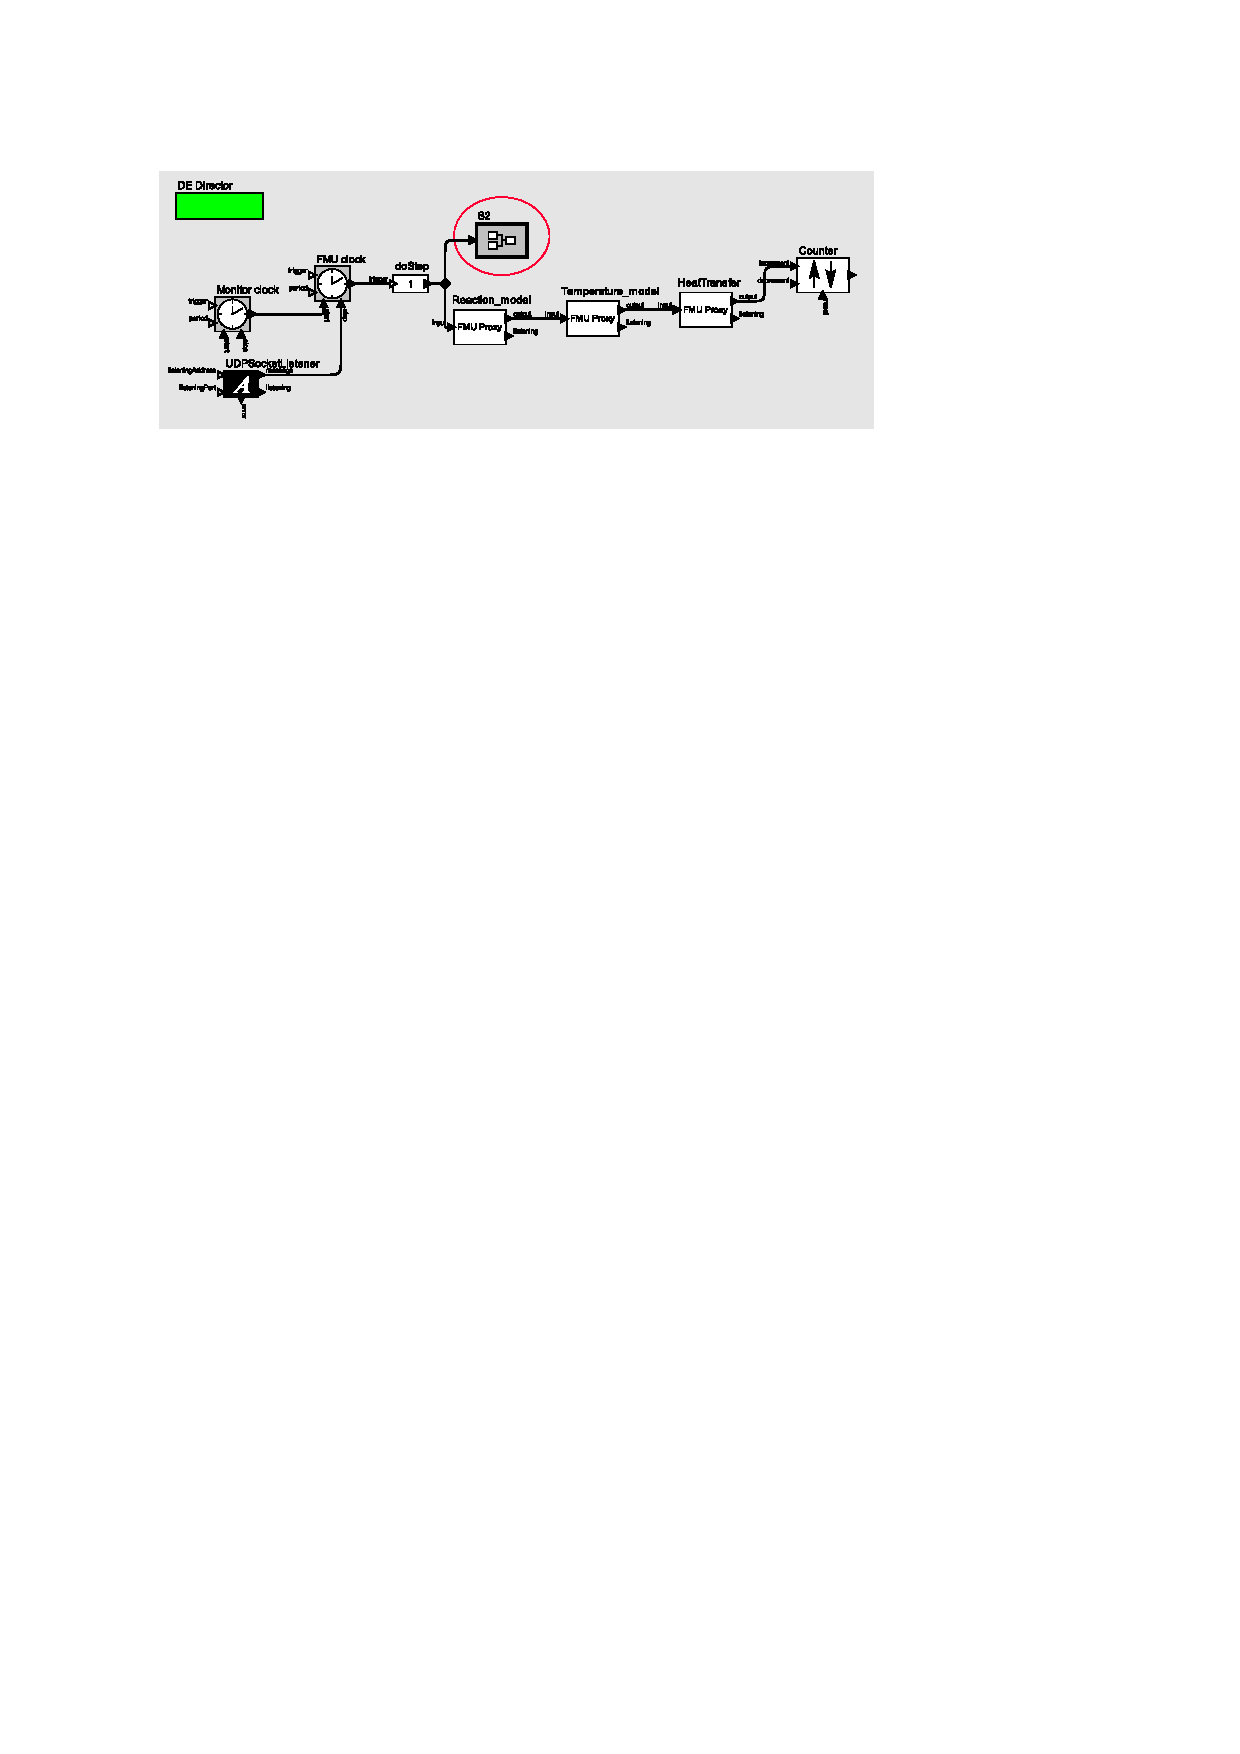
\includegraphics[scale=1.1]{figures/s2_pt_composite.pdf}
  \caption{The encapsulation of S2}
  \label{fig:s2_pt_composite}
\end{figure}

The internal implementation of \textbf{S2} is shown in Figure \ref{fig:s2_pt_internal}, where the \texttt{FMU Proxy} is triggered by the \texttt{FMU clock}---shared by \textbf{S1}---from the outside. Then the computed command is sent to a remote actuator webhook using the REST client actor.

\begin{figure}[hbt!]
  \centering
  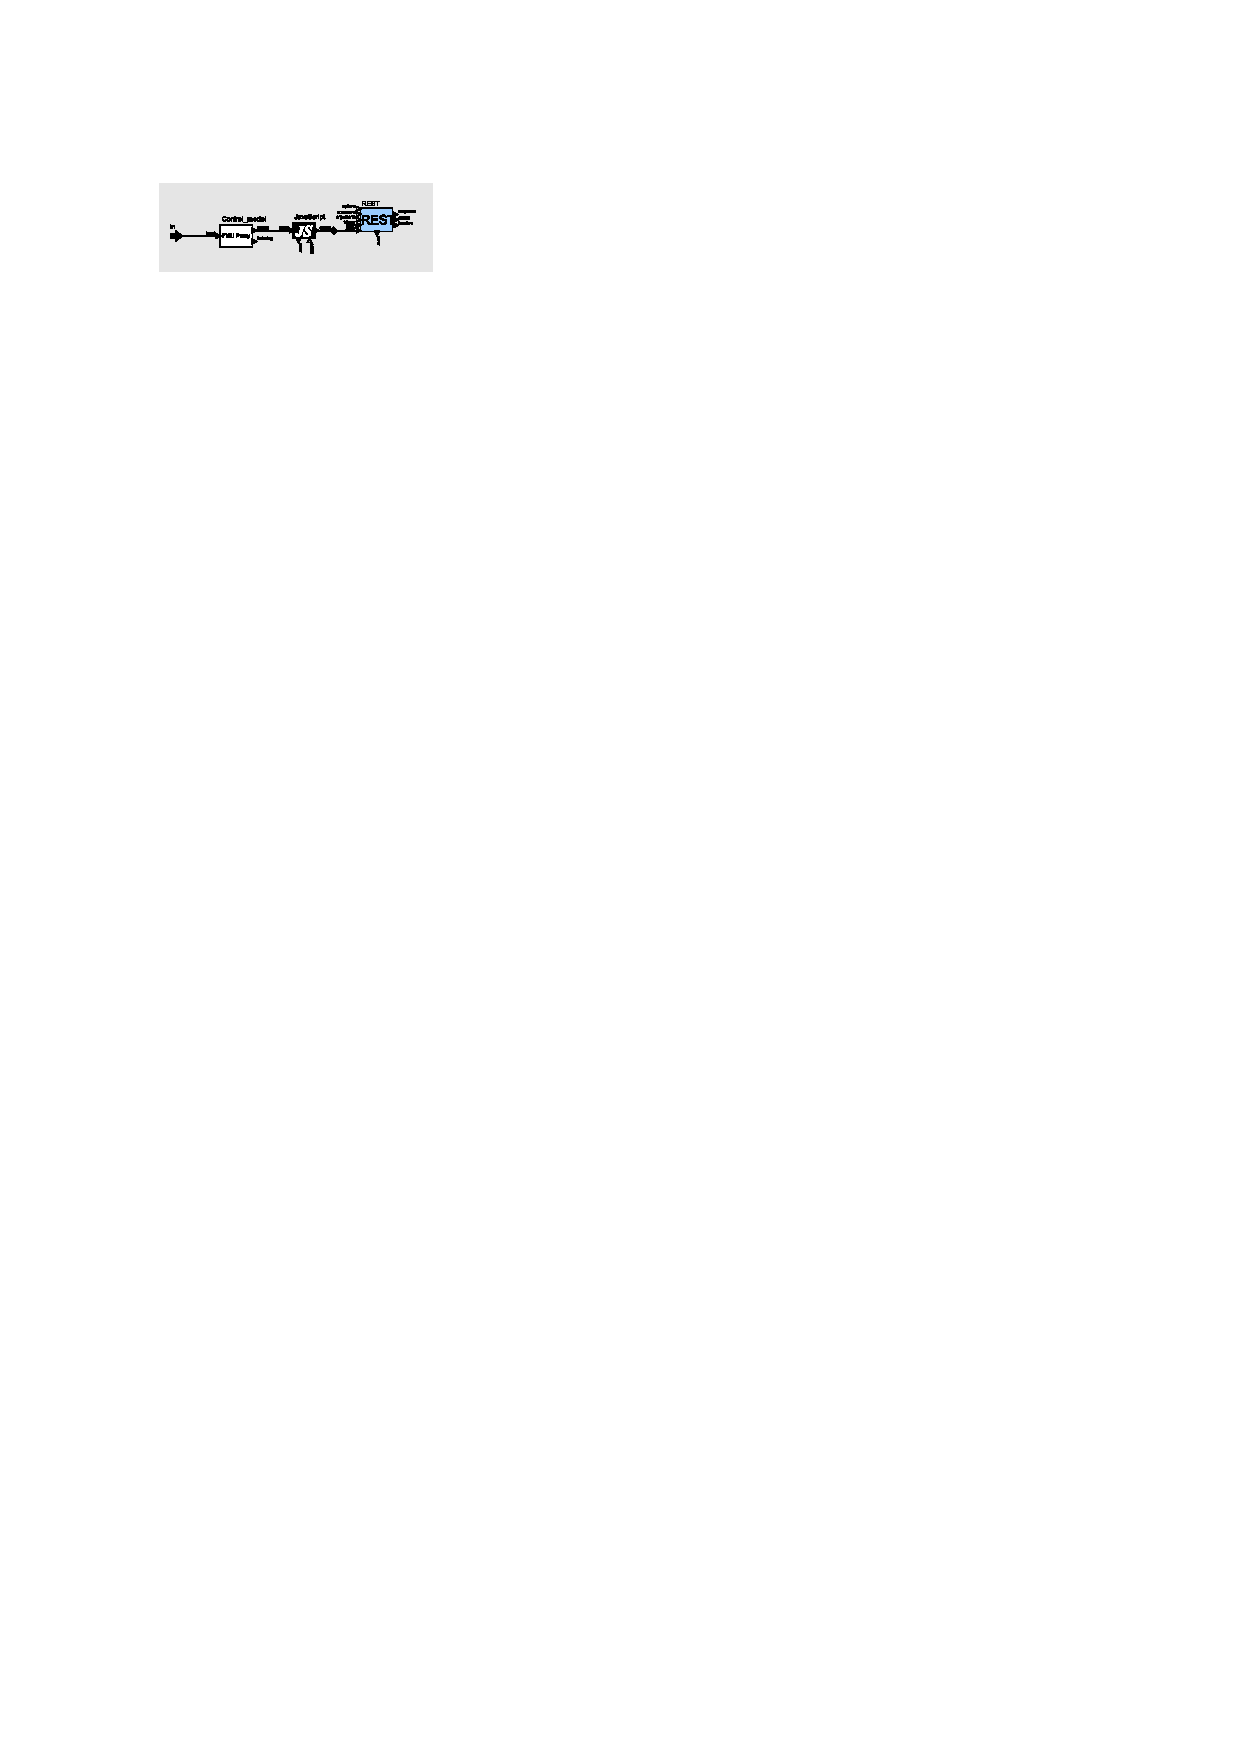
\includegraphics[scale=2.1]{figures/s2_pt_internal.pdf}
  \caption{S2 design in Ptolemy II}
  \label{fig:s2_pt_internal}
\end{figure}

We conclude the implementations for \textbf{S1} and \textbf{S2} here. In the next chapter we will compare the frameworks' characteristics, performances, and non-functional properties.


\clearpage

\chapter{Evaluation and Discussion}\label{ch:discussion}
In this chapter, we revisit the proposed KPIs of the two services, and evaluate them in regards to the framework implementations. As explained in Chapter \ref{ch:methodology}, the KPIs are meant to verify the requirements of the services, so we could confirm the effectiveness of the frameworks. After that, a summary will be made to compare the frameworks in overall.

\section{S1 KPIs evaluation}
In \textbf{S1} (Production Prediction), four KPIs are highlighted (see also Table \ref{tab:s1kpi}), namely, \textbf{level of automation}, \textbf{updating delay}, \textbf{data history}, and \textbf{modifiability}. 

\subsubsection{KPI1: level of automation}
This KPI measures the number of manual steps required in order to support the operations of the framework. Generally, fewer steps are desired as it indicates the framework has a higher level of automation. The steps referred here contribute toward the requirement \textbf{R1}---validate the model states with real-time data.

In practice, the notion of ``step" depends on the architecture of individual frameworks and the use cases. For the purpose of comparison, we have identified four primary actions that occur in \textbf{R1}: data collection, data integration, model scheduling, and status reporting. The manual steps contribute to the automation of these actions in runtime. Note that the actions we have identified here are specific to the microbrewery context. For other use cases, more or fewer actions might be needed to achieve the outcome.

In TwinOps, the collection of monitoring data is handled automatically by Kafka. The openness of the SSP format---which defines the connections between models---allows the internal variables of models to be accessed easily. The core validation process, which includes validating the simulations against real-world data and reporting the new model states, takes place in the CI/CD pipelines. The pipelines are configured in the YAML file by the user ahead of executions. This configuration is the only manual step in the full process cycle. In other words, once the pipelines are pre-configured, the rest of the process should run automatically.

As an IoT-based framework, ThingsBoard uses application-layer protocols that enhance the simplicity in data collection, shielding the user from handling low level communications. However, due to the lack of native model editor supports, the monitoring data and the models are integrated externally to the platform environment during the running of the system. In consequence, a manual step is required for interfacing back to the platform after the integration is complete. Because of that, it poses another disadvantage such that scaling could be hindered as more models are introduced. The model scheduling and its status reporting are automated using \textit{rule chains}. The user is tasked to manually define the \textit{entities} (e.g., sensors) and their \textit{relations} (e.g., sensors are \textit{contained} by the models) before the beginning of \textit{rule chains}. In overall, the two manual steps identified here are interfacing the model editor and entity provisioning. 

Ptolemy II comes with an actor type Accessors that supports external communication. In term of data integration, both the built-in \texttt{FMUImporter} and the \texttt{FMU proxy}---which we opted for---bear resemblance to a blackbox. It means that accessing the internal model states is difficult to achieve unless with an external model editor. Hence, facing the same situation as ThingsBoard, the user has to implement an additional interface. The model scheduling is automatically maintained by the MoC director and the clock actors. As we mentioned earlier, Ptolemy II lacks a data storage feature that suites our DT service. Therefore the user has to establish data logging externally, Kafka has been manually integrated for this task. All things considered, the two manual steps are interfacing the model editor and interfacing the data manager.

Table \ref{tab:kpi1compare} shows a summary of manual steps in each framework. TwinOps is the most automated framework, followed by ThingsBoard and Ptolemy II, as both require some patchworks by the user for different stages of the operation. As we can see, TwinOps enables the user to manage an extensive range of configuration options prior to runtime, it leads to less inconveniences in term of making further patchworks in various parts of the system, as in the cases with the other two frameworks. Additionally, it could also mean less risks for human errors to occur.

\begin{table}[hbt!]
\centering
\begin{tabularx}{\textwidth}{|X|p{3.5cm}|p{3.5cm}|p{3.5cm}|}
\hline
\textbf{} & {TwinOps} & {ThingsBoard} & {Ptolemy II} \\ \hline           
\textbf{Manual steps} & Pipelines configuration & (1) Interfacing model editor. (2) Entity provisioning. & (1) Interfacing model editor. (2) Interfacing data manager. \\ \hline             
\end{tabularx}
\caption{S1 KPI1 comparison}
\label{tab:kpi1compare}
\end{table}

\subsubsection{KPI2: updating delay}
We define updating delay as the time between when the framework has collected all required data and when the updated model states have been computed. Therefore, each updating cycle begins from the completion of data collection and ends in the completion of new model states output. We find that one of the main factors influencing this KPI is the communication style of the orchestration, for instance, whether it relies on external protocols or using in-memory communication. Another factor is due to the initialization process. For cloud based platforms this relates to the initiation of the ``workers" and to their load balancing algorithm, i.e., the allocation of computational power. For platforms that are hosted in local premises, loading the required resources also contributes to delays.

\begin{figure}[hbt!]
  \centering
  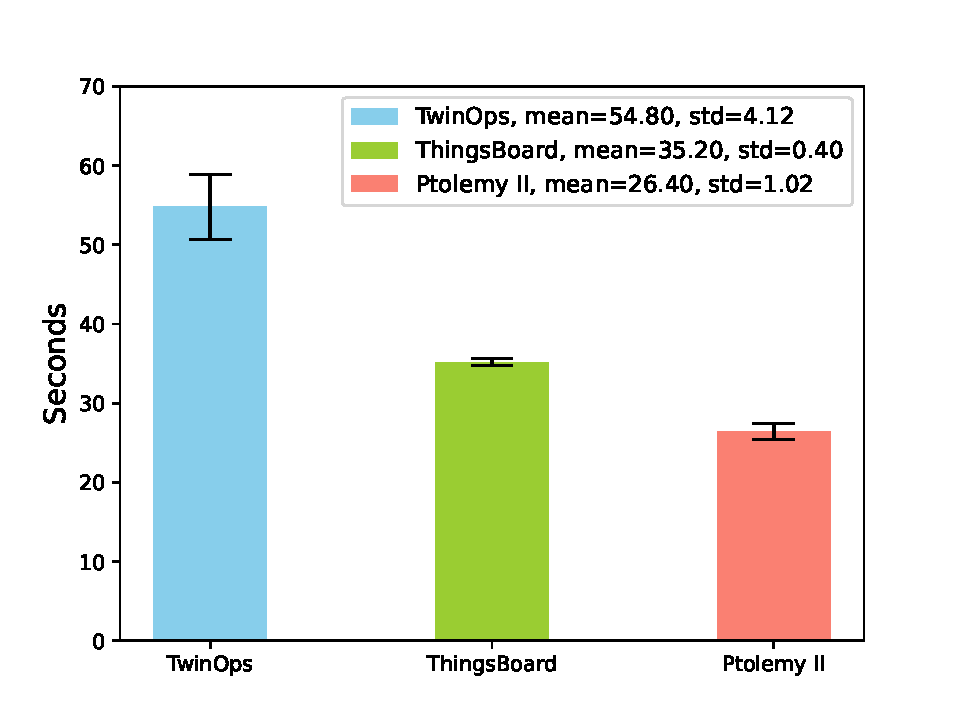
\includegraphics[scale=0.5]{figures/s1kpi2.pdf}
  \caption[S1 KPI2: updating delay]{S1 KPI2: updating delay mean value and standard deviation}
  \label{fig:s1kpi2}
\end{figure}

Figure \ref{fig:s1kpi2} shows the statistics of five updating cycles presented in a bar chart. We observe that TwinOps has the highest mean delay time as well as the greatest standard variation. This is due to the CI/CD engine being hosted in the cloud (as with most popular CI/CD engines in the market), such that it is subject to a user's pricing plan, which results in different load balancing strategies imposed by the cloud server. To keep the measurement consistent, the five updating cycles all use the same free-tier plan.

In ThingsBoard, the orchestration communication utilizes a combination of remote procedure call (RPC) and RESTful protocol. Both are  high level protocols that suggest more packet overhead. This results in the moderate delay time we have seen. In most cases, protocol APIs tend to use buffering techniques to ensure QoS, including mitigation of delay time variance. In ThingsBoard we have already seen that being imposed by the background process as \texttt{TbServiceQueue} in Chapter \ref{ch:implementation}.

For Ptolemy II, given that we use the \texttt{FMU proxy} instead of \texttt{FMUImporter}, a communication overhead is expected. Surprisingly, the mean delay time is the lowest among all the tested frameworks. There are a few hypotheses to this. Firstly, \texttt{FMU proxy} uses UDP interface for communications, which is a low level connectionless protocol. Therefore it is exempted from delays incurred by the excessive handshakes often found in connection-oriented or high level protocols. Secondly, Ptolemy II holds all of its processes together in an unified software package, meaning it needs few external communications or memory fetching beyond the program scope, in contrast to the modular architecture of TwinsOps or ThingsBoard.

It is important to acknowledge a limitation of this KPI measurement, which is that since the frameworks permit quite flexible building block choices for the user, the technologies adopted in the framework may considerably affect the system timing behaviors. For example, one might use a CI/CD engine that is not cloud-based and possibly achieve a much lower delay time; or one could opt for another M2M protocol that is not built-in to ThingsBoard, thus increase or decrease the overall communication latency. The KPI results presented here should be regarded as a reflection of our particular microbrewery DT setup, serving as a reference instead of an absolute judgment.

\subsubsection{KPI3: data history}
Data history concerns the amount of historical data ready to be used for the service. For context, the data are being used for computing future heat transfer in \textbf{S1}.

In TwinsOp, the user is able to add steps inside the CI pipeline that archive data as artifacts. On the other hand, in the CD pipeline, as we have discussed, data are containerized as images and stored in the online repository. ThingsBoard framework provides native data storage that is integrated with the \textit{rule engine}, such that the historical model states and events are constantly recorded in background. Ptolemy II on its own lacks an efficient data management system. However, we manage to solve that shortcoming by integrating the Kafka service.

In overall, all three frameworks are able to retain all historical data for the full lifecycle of the service.

\subsubsection{KPI4: modifiablility}
This KPI concerns two main aspects: the configuration of model initial values; and the configuration workflow of model executions. Our use case reveals that each framework offers varying degrees of configurability before and after startup, as discussed below.

Due to the modular nature of TwinOps, a user can customize all stages of the framework workflow, including the control of the model executions. In terms of initial value setting for the models, it could be accomplished in the SSP file. Table \ref{tab:twopconfig} summarizes the initial configuration options accessible by the user. Once all the configuration options are settled, the DT should be able to operate automatically.

\begin{table}[hbt!]
\centering
\begin{tabularx}{\textwidth}{|p{1.5cm}|p{3.5cm}|p{3.5cm}|X|}
\hline
\textbf{Type} & {SSP} & {YAML} & {Dockerfile} \\ \hline           
\textbf{Format} & \texttt{.ssp} & \texttt{.yml} & No file extension  \\ \hline
\textbf{Scope} & models editor & CI/CD engine & CI/CD engine \& container repository \\ \hline
\textbf{Purpose} & Define the execution flow and data dependencies between FMUs & Validate the updated model states & Deploy to the target platforms \\ \hline    
\end{tabularx}
\caption{TwinOps initial configurations overview}
\label{tab:twopconfig}
\end{table}

Likewise to TwinOps, the ThingsBoard framework is also highly customizable, such that all workflow stages can be configured at the beginning. Furthermore, the \textit{entity management} provides the option to set initial values and attributes to the model entities. The summary of configuration options is shown in Table \ref{tab:tbconfig}.

\begin{table}[hbt!]
\centering
\begin{tabularx}{\textwidth}{|p{1.5cm}|p{3.5cm}|p{3.5cm}|X|}
\hline
\textbf{Type} & {CSV} & {JSON} & {Configuration} \\ \hline           
\textbf{Format} & \texttt{.csv} & \texttt{.json} & \texttt{.conf}  \\ \hline
\textbf{Scope} & Entity management & Profile \& rule chain \& dashboard & ThingsBoard backend services\\ \hline
\textbf{Purpose} & Provision entities and define their relations & Setup device profiles, rule chains, and dashboards & Set parameters to ThingsBoard background processes such as memory allocation, timeout, etc.\\ \hline    
\end{tabularx}
\caption{ThingsBoard initial configurations overview}
\label{tab:tbconfig}
\end{table}
 
In contrast, the architecture of the Ptolemy II workflow is relatively monolithic and closed compared to the other two frameworks. Designing is done in the GUI of the software, where the operator performs drag-and-drop on the icons representing directors and actors, though there is the option to import or export the design in XML format. The operator could alter the execution flow by choosing the MoCs, represented by directors. Although the MoCs account for the timing progression of models, they do not address the configurations for the data collection before the model update and the data storage after the model update. It suggests the modifiablility of Ptolemy II is inadequate to cover the entire workflow for the service. Many actors in Ptolemy II do not support initialization of model parameters. Therefore, a workaround has to be made by using input variables. Although it does not affect the functionality, potential confusions may arise for the downstream user who does not develop the models in first hand.

\section{S2 KPIs evaluation}
In \textbf{S2} (Production Control), two KPIs (see also Table \ref{tab:s2kpi}) will be evaluated, which are \textbf{traceability} and \textbf{latency}. 
\subsubsection{KPI1: traceability}
In context, the traceability is concerning how much information is available to the operator which they can use to evaluate the effects of the DT's controlling actions.

In TwinOps, the building blocks in each workflow stage are only loosely coupled, they are each an independently deployable module. As a result, the trace of a model's behaviors can be quite scattered. When progressing through stages, the model artifacts, such as connection links, parameters, and states, tend to undergo format transformations that will lose some explicitness of the traces.
To illustrate, the models topology is visualized in the model editor stage, but in the CI/CD stage it becomes a part of pipeline instructions that is no longer easily readable by humans. From the CI/CD stage to the containerizing stage, another transformation occurs as the pipeline instructions are brought into a container image which requires another service (e.g. docker) to run. To sum up, the consistency of trace explicitness is often lost during the transfer of data ownership from one stage to another.

As we have seen in the dashboard demonstration in Section \ref{sec:s2demo}, the ThingsBoard framework handles the system traceability very well. It is attributed to the highly integrated operability between the \textit{rule engine}, the data storage, and the real-time dashboard. When data ownership is transferred between them, the framework ensures the data properties, e.g., timestamps, data types, etc, remain consistent throughout. Therefore, one is able to easily trace an effect back to its root cause.

In theory, Ptolemy II supports the transfer of data ownership, meaning an actor will gain full controls of data once receiving from another actor. However, this is more true when two actor types are alike. When the types are significantly different, such as between a server actor---which sends and receives internet packets---and a mathematical operation actor, all kinds of errors may occur. The user has to make sure the conversion is done properly. As more kinds of actors are adopted to support the growing DT service, it becomes harder to scale up this kind of pairing conversion. Eventually making the system traces harder to track.

\subsubsection{KPI2: latency}
This KPI measures the latency between the finishing of model updates and the completion of the control triggering. It indicates the responsiveness of the framework in dealing with VE-PE communications. Figure \ref{fig:s2kpi2} shows the statistics of five measurements.

It can be seen that TwinOps has the highest mean and standard variation. It is again due to the load balancing mechanism managed by the CI/CD host server. ThingsBoard and Ptolemy II have similar mean latency, but the former clearly has the lower of the two variances.

This KPI suffers the same limitation as \textbf{S1 KPI2}. The timeliness is sensitive to the high variability of technology choices made by the user. Although we can see a general pattern here that a centralized system such as Ptolemy II has lower latency than distributed systems like TwinOps.

Aiming for low mean latency and low variance are two particularly important properties for a time critical system, even though the microbrewery DT is not one such system. They affect the bound for worst case execution time (WCET), which is a determining factor in schedulability analysis, i.e., the computation deciding whether a set of tasks are able to meet the deadline in a real-time system.

\begin{figure}[hbt!]
  \centering
  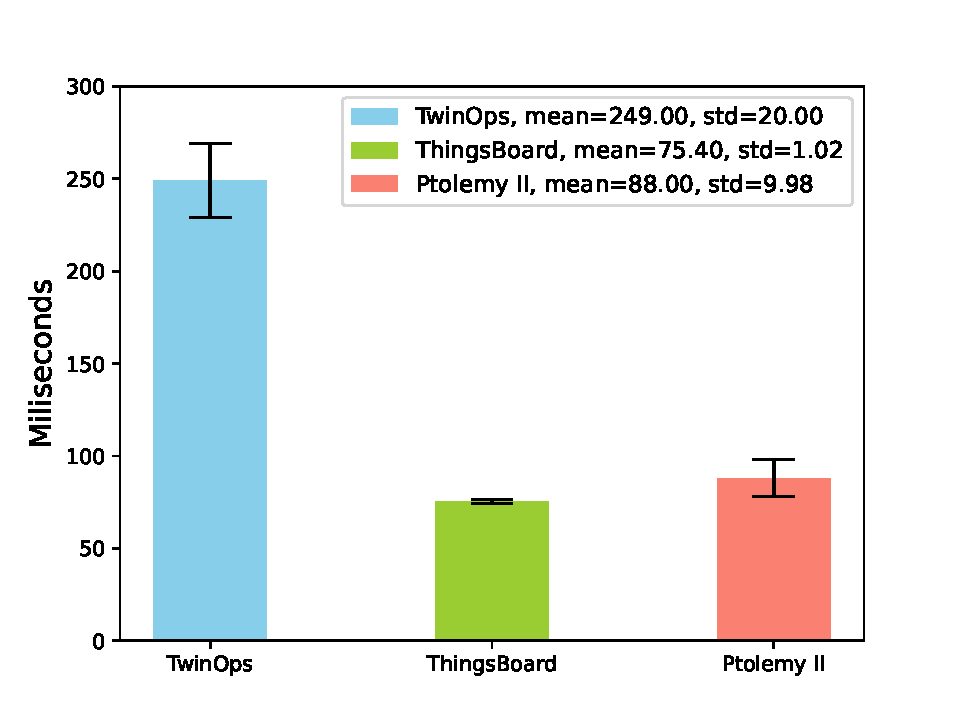
\includegraphics[scale=0.5]{figures/s2kpi2.pdf}
  \caption[S2 KPI2: latency]{S2 KPI2: latency mean value and standard deviation}
  \label{fig:s2kpi2}
\end{figure}

\section{Summary of framework comparison}
This section summarizes the most significant findings about the frameworks in terms of integration and orchestration. Table \ref{tab:framecompare} shows a side-by-side comparison. The rows represent the categories generalized from the KPIs and the requirements to a broader scope; the columns list the three frameworks. Most categories below have been introduced in the earlier chapters. ``Data transformation" covers the ability to transform the data to other forms or formats for the subsequent stages within the workflow, or for storing in case of future usages. ``Traceability", as explained in the earlier section, is an aspect of data ownership. We have decided to compare the traceability instead of the greater scope (ownership), as it is a narrower---more focused---aspect, making it easier to compare between the considerably different framework styles in this project.
 
\begin{table}[hbt!]
\centering
\begin{tabularx}{\textwidth}{|X|p{3cm}|p{3cm}|p{3cm}|}
\hline
 & \textbf{TwinOps} & \textbf{ThingsBoard} &  \textbf{Ptolemy II}\\ \hline    
\multicolumn{1}{|l|}{\textbf{Integration}} & \multicolumn{3}{c|}{}\\ \hline           
{Configurability} & high & high & medium \\ \hline
{Data transformation} & high & medium & medium \\ \hline
{Traceability} & complex & simple &  simple (but inefficient) \\ \hline
{Modularity} & high & medium & low \\ \hline   
\multicolumn{1}{|l|}{\textbf{Orchestration}} & \multicolumn{3}{c|}{}\\ \hline  
{Workflow automation} & high & medium & low\\ \hline
{Timeliness} & slow & fast & fast\\ \hline
{Managing diversity} & good & good & good (but requires external add-ons) \\ \hline 
\end{tabularx}
\caption{Framework comparison}
\label{tab:framecompare}
\end{table} 
 
Regarding the integration aspects, TwinOps is highly configurable and modular, credited to its multi-stage architecture; its data can be transformed effectively to adapt to different stages of the workflow. However, the same features make it difficult to conduct explicit ownership transfer of model artifacts, meaning the methods for data accessing may vary considerably in different stages. This can hinder the traceability of the DT behaviors. ThingsBoard also has high configurability. The components within the framework are more cohesive, resulting in a more consistent data ownership and medium modular potential. Ptolemy II, being a self-contained software, has limited---under the DT context---configuration options and limited modularity. Some data transformation can be performed by the actors, although it is often not necessary as the processes in the workflow are already tightly coupled. The actor-orientated architecture is conducive to a consistent data ownership although extra patches, such as data format conversions from one actor type to another, are often needed. That makes the tracing of the system become inefficient.

For the orchestration aspects, TwinOps is able to attain the highest automation; we argue it is correlating to the extensive preliminary configurations. It is quite slow, because the cloud-based CI/CD engine focuses on the ``continuity" angle instead of the ``speed" angle of operation. ThingsBoard takes advantages of its IoT networking backends, resulting in decent automation and decent speed. For Ptolemy II, the workflow requires some manual implementations from the user to automate. It is fast since the framework is relatively more centralized, thus its components suffer less from communications and synchronizations penalty.

Finally, all three frameworks manage to satisfy all requirements of the DT services, even though their KPIs show the weaknesses and caveats that the user has to keep in mind of during the development process. The frameworks are capable of managing diverse types of entities in the microbrewery DT, presuming the requirement for time criticality is not strict, as is the case with fermentation processes.

\clearpage

\chapter{Conclusion and Future work}\label{ch:conclusion}
\section{Conclusion}
This project contributes to the identification of the important aspects of integration and orchestration of DT models: (1) We identified the related literature, relevant requirements and KPIs. (2) We have investigated three distinctive frameworks which we believed suitable for DT developments and tested them for a microbrewery DT. In consequence, we have obtained findings that can answer the research questions:
 
\begin{itemize}

  \item \textbf{RQ1}: What are the key ingredients for integration and orchestration of models in different services for a microbrewery DT? \\ \newline
	The microbrewery DT concerns a weeks-long bio-chemical process. Many of its process variables are inferential rather than directly detectable. Taken these characteristics together, the production prediction service (\textbf{S1}) has to inter-operate several numbers of entities effectively for a prolonged time frame in order to generate reliable predictions. We argue that a multi-stage or pipelining architecture can resolve the differences across the entities sufficiently well. Since it opens up more ways to combine integration and orchestration techniques by allowing the developer to add or swap individual stages. In this type of design, the emphasis is on the configurability, and modularity of individual stages. Working with flexible building blocks alleviates many constraints for the user when integrating distinctive models.
	
	Another implication of early stage configurations is that it correlates with high level of automation during the operation phases. Our results have shown that extensive initial setups of the DT system reduce the number of orchestration and integration steps that need operator interventions later, thus mitigating the chance of human errors. 
	
	In the production control service (\textbf{S2}), the operator is most interested in knowing the effect of the control actions. Therefore, the traceability within the system becomes particularly important. The traceability is dependent not only on data availability, even more so the semantics and explicitness of data need to be consistent for the operator to access them easily afterward. Therefore, the trade-off between the degree of data transformations---for the purpose of adapting in different systems/hardwares, etc---and data consistency need to be considered. The trade-off occurs as the data format is transformed in numerous workflow stages, the means of accessing the data may also change repeatedly. That leads to a higher chance of improper data retrieval or negligence by the user, which eventually undermines the data consistency.      
	
	Coming back to the research question, the key ingredients are configurability, modularity, and traceability. 
	
  \item  \textbf{RQ2}: How can these ingredients be generalized to benefit other application domains? \\ \newline
  Most of the previously mentioned points will still hold in the DTs of other fields, as long as their development processes are also guided by MDSE and the 5D model. As these two concepts provide a structured view of a complex system, guiding developers toward the requirements and promoting the usage of recurring ingredients in order to eliminate rework. Nevertheless, in some circumstances, if a certain DT requires real-time processing within a very short cycle time, e.g., seconds, then the system timeliness becomes a more important issue. Our findings indicate that a monolithic orchestrating style has shorter delays than the distributed counterparts, mainly because it has inherently fewer communication points and synchronization barriers.
  
  As a result, when creating DTs for a new application domain, one should identify the unique requirements, and then utilize the MDSE methods and 5D model to incorporate the unique parts into the known patterns based on the past designs.
   
  \item  \textbf{RQ3}: In what circumstances do the selected frameworks best fit these ingredients?   \\ \newline  
  From this project we have learned that the choice of frameworks depends highly on the specific use case. If one's use case stresses on minimizing manual integration and verification by humans, then TwinOps will be best suited as its CI/CD paradigm is made for that very purpose. For the use cases where the models are physically separated on different machines, ThingsBoard will be a wise choice as it is supported by the underlying IoT network. We consider Ptolemy II falls short of several crucial integration aspects as a DT framework, for its lack of data management components and its relatively inflexible user modifiability. However, it serves as a good experimentation framework for testing orchestrations thanks to the variety of MoCs it supports. Apart from that, the monolithic architecture of Ptolemy II allows the fastest overall speed, useful for dealing with time critical applications.
  
\end{itemize}

To summarize, in this project we found out the frameworks of distinguishing styles can all accomplish the requirements of our microbrewery DT services. This is an encouraging finding because it allows users from different disciplines to choose what is best fit for their use cases and backgrounds---despite the different shortcomings within the individual framework to be overcame. We learned that multi-stage frameworks have the benefit of accepting more kinds of integration and orchestration techniques, but come with the cost of potentially slower system speed, and more complex system behavior traces, as the data exchanges across stages may be implemented differently. On the contrary, monolithic frameworks are less flexible with especially the integration aspects, but they have the advantage of faster system responsiveness. Ultimately, developers may take these findings as a guidance when designing their own frameworks for DTs of different use cases.


\clearpage
\section{Future work} \label{sec:futurework}
For the research on frameworks, we can start looking for extension modules/packages that may compensate for the weaknesses in each framework, just as we have shown that Kafka was adopted as a data management tool to support the frameworks that lack it. The immediate focus will be on the property of time criticality. We are interested in how the framework determines if the operations can meet the deadlines in a real-time scenario, and how can it be guaranteed. Time criticality is prioritized because it is a crucial factor for many systems such as automotives that have safety requirements---unfortunately not the case of a microbrewery.

As for the microbrewery case study, there four services proposed, but only two (\textbf{S1} and \textbf{S2}) have been implemented, and they both fall within the \textit{manufacturing phase} of the product life cycle. In this phase the main concern is the final production yield. 

The other two services, \textbf{S3} (what-if scenarios) and \textbf{S4} (predictive maintenance) belong to the \textit{service phase} which holds a different kind of objective, especially more focusing on the user-orientated aspects than the \textit{manufacturing phase}. Because of that, we predict a new set of challenges and findings will arise, making them worthy of further investigations. Table \ref{tab:s3req} and \ref{tab:s4req} present the tentative requirements for \textbf{S3} and \textbf{S4}.

\begin{table}[hbt!]
\centering
\begin{tabularx}{\textwidth}{|p{1cm}|X|}
\hline
\multicolumn{2}{|c|}{\textbf{Requirements}} \\
\hline
\textbf{ID} & \textbf{Requirement description} \\ 
\hline            
R1 & The scenario-specific data shall be handled separately from the master data. \\ 
\hline
R2 & The scenarios can be added, reset, and removed without affecting the master schedule. \\ 
\hline
R3 & The iterations of scenario may be stored and managed under version control.\\ 
\hline
\end{tabularx}
\caption{S3 requirements}
\label{tab:s3req}
\end{table}

\begin{table}[hbt!]
\centering
\begin{tabularx}{\textwidth}{|p{1cm}|X|}
\hline
\multicolumn{2}{|c|}{\textbf{Requirements}} \\
\hline
\textbf{ID} & \textbf{Requirement description} \\ 
\hline            
R1 & Dynamic data acquisition shall be used to update the static attributes in the predictive model. \\ 
\hline
R2 & Real-time measurements and simulated results shall be used in the retrofitting of the predictive model. \\ 
\hline
R3 & Data pruning and refining should be done before applying them to the predictive model \\ 
\hline
\end{tabularx}
\caption{S4 requirements}
\label{tab:s4req}
\end{table}

In the requirements for \textbf{S4} we can see a large proportion directs to the data processing aspect of the predictive model, it is because we plan to adopt a data-driven modelling approach for this service. It will be unlike the mechanistic models used in \textbf{S1} to \textbf{S3}, as the data quantity and quality will have greater influences on the final results.

\newpage
Likewise the KPIs for \textbf{S3} and \textbf{S4} are also proposed in Table \ref{tab:s3kpi} and Table \ref{tab:s4kpi}. Note that these are still in early stage of design therefore are subject to substantial refinements.

\begin{table}[hbt!]
\centering
\begin{tabularx}{\textwidth}{|p{1cm}|p{2cm}|X|p{2cm}|}
\hline
\multicolumn{4}{|c|}{\textbf{KPIs}} \\ 
\hline
\textbf{ID} & \textbf{Name} & \textbf{Description} & \textbf{Verifies} \\ 
\hline
KPI1 & Scalability & To what extent are the additional space and time bounded. & R1, R2, R3 \\ 
\hline
KPI2 & Accessibility & Are the model instances of the scenarios easily accessible to the operator. & R1, R3 \\ 
\hline
KPI3 & Modularity & Is changeover of the setup for each scenario easily adaptable. & R2 \\ 
\hline
\end{tabularx}
\caption{S3 KPIs}
\label{tab:s3kpi}
\end{table}

\begin{table}[hbt!]
\centering
\begin{tabularx}{\textwidth}{|p{1cm}|p{2.5cm}|X|p{1.5cm}|}
\hline
\multicolumn{4}{|c|}{\textbf{KPIs}} \\ 
\hline
\textbf{ID} & \textbf{Name} & \textbf{Description} & \textbf{Verifies} \\ 
\hline
KPI1 & Accuracy & What is the error of the predictive model against real-world measurement. & R1, R2 \\ 
\hline
KPI2 & Data sufficiency & How missing data may affect the overall performance of predictive model. & R1, R2 \\ 
\hline
KPI3 & Data quality & How much volume, variety, and veracity of the data is lost as the result of transferring
and merging. & R3 \\ 
\hline
\end{tabularx}
\caption{S4 KPIs}
\label{tab:s4kpi}
\end{table}

\newpage


\clearpage


\bibliographystyle{IEEEtran}
\bibliography{IEEEabrv,references}


\clearpage

%\addcontentsline{toc}{chapter}{Appendix}
\renewcommand\chaptername{Appendix}
\begin{appendices}
\chapter{DT workflow in bioprocessing domains} \label{apd:workflow}
The 5D model introduced in Section \ref{sec:overview} provides a reference for entity management in DTs. Nonetheless, in the field of bioprcessing, there are other aspects at which one often finds important to inspect. One of them is the maturity of the DT models. For this reason, Udugama et al. \cite{Udugama2021} propose a five-step workflow (illustrated in Figure \ref{fig:fivestep}) to implement a DT of bioprocessing domain. The workflow progresses in increasing order of mathematical complexity and functional requirements.

\begin{figure}[hbt!]
  \centering
  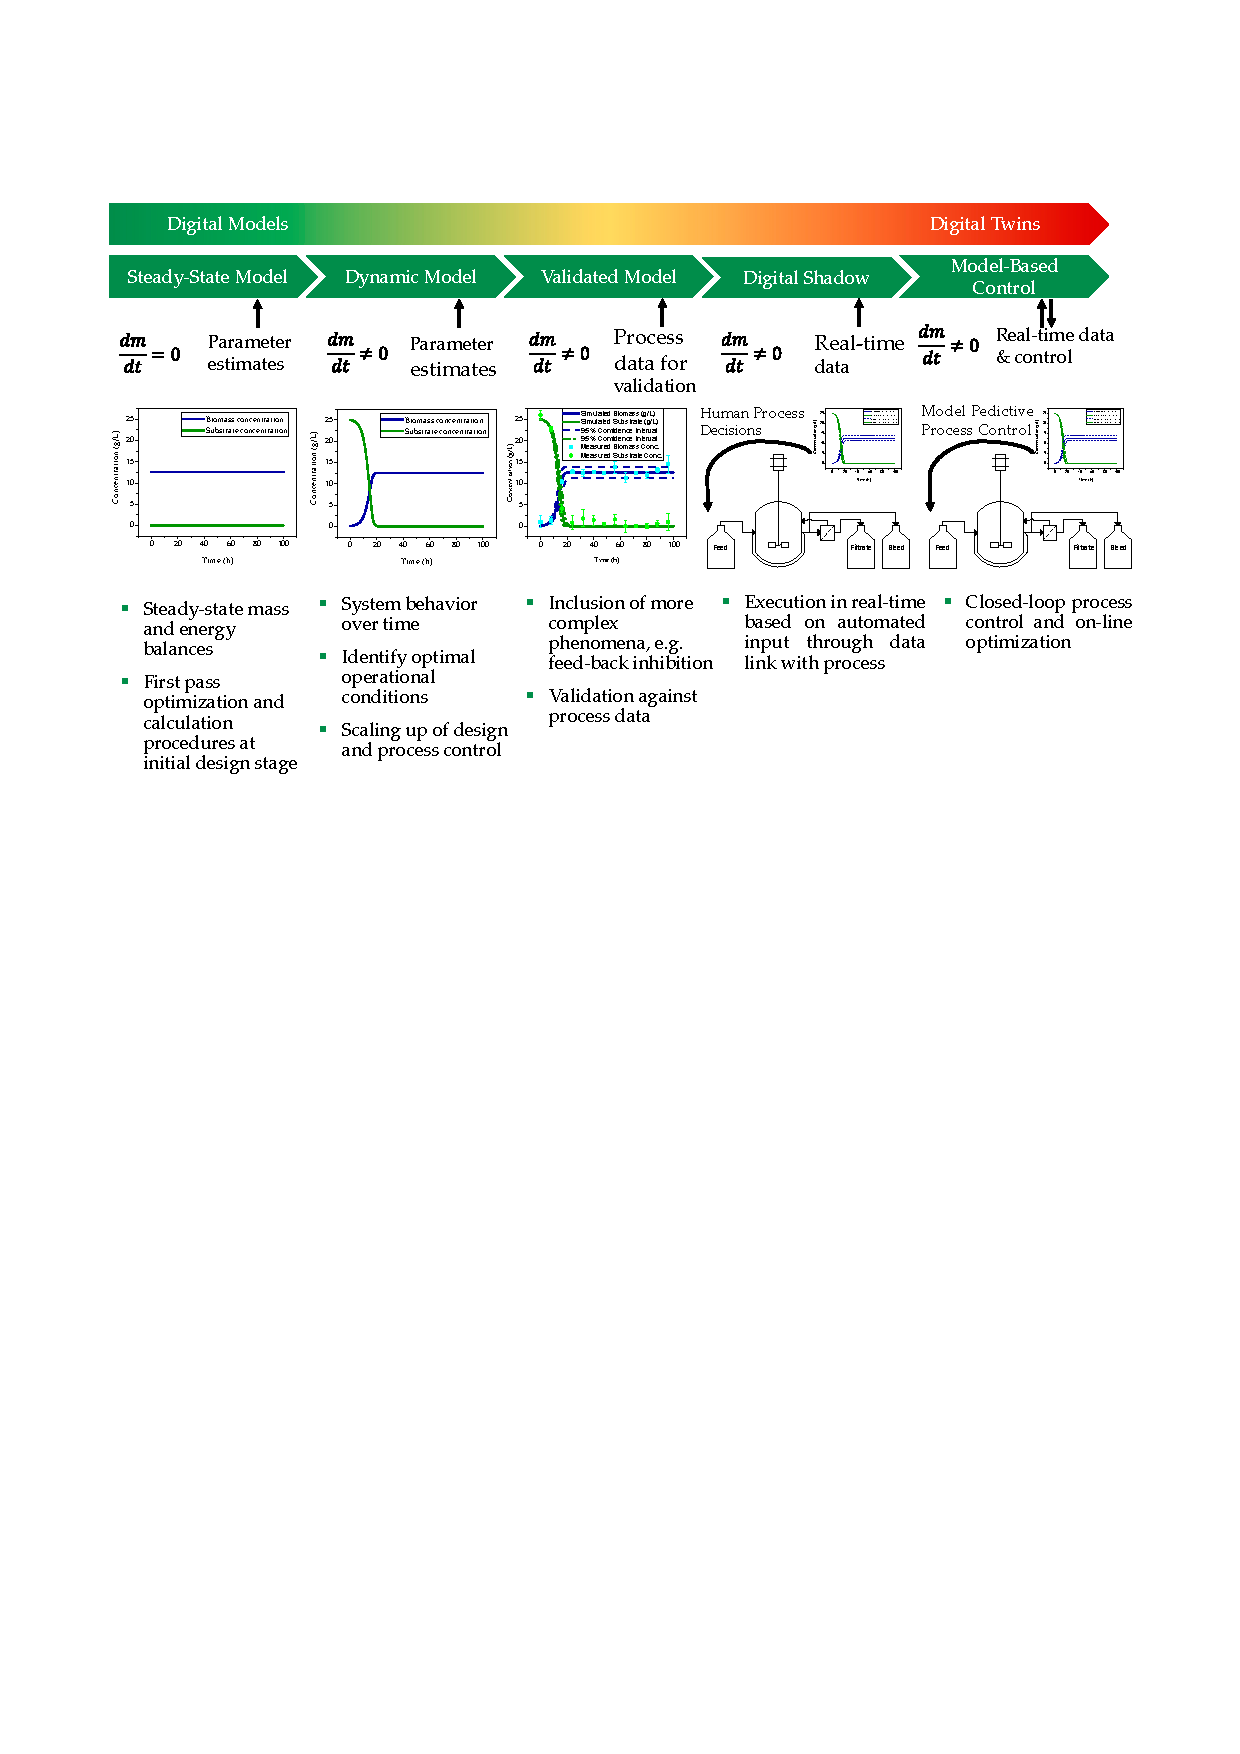
\includegraphics[scale=0.8]{figures/fivestep.pdf}
  \caption[The five-step implementation]{The five-step implementation. This workflow has been adopted in a design of DT for monoclonal antibodies manufacturing \cite{Helgers2022}.}
  \label{fig:fivestep}
\end{figure}

\begin{enumerate}
  \item \textbf{Steady‑state model}: consisted of a mass and energy balance of the different key compounds in a reaction. These models are mathematical expressions of a process
that are not time-dependent and hence carry no accumulation
term.
  \item \textbf{Dynamic model}: contains time-based derivative terms on all variables of interest.
  \item \textbf{Validated model}: extends the capabilities of dynamic process models, such that it needs to be validated against process data obtained from an actual physical process.
  \item \textbf{Digital Shadow}: consistent with the definition of Section \ref{sec:overview}; An one-way real-time monitoring model.
  \item \textbf{Digital Twin}: consistent with the definition of Section \ref{sec:overview}; A two-way real-time monitoring and control model.
\end{enumerate}

\chapter{Microbrewery physical workbench} \label{apd:workbench}
This section presents the workbench setup of the microbrewery DT. All the equipment are settled in a typical living room. A Raspberry Pi is used for aggregating all sensor data (except for those come from Airlock, they use a dedicated webhook server which is included as a part of product supports) before further processing in the DT. Figure \ref{fig:workbench_fermenter} shows the fermenter setup. 

\begin{figure}[hbt!]
  \centering
  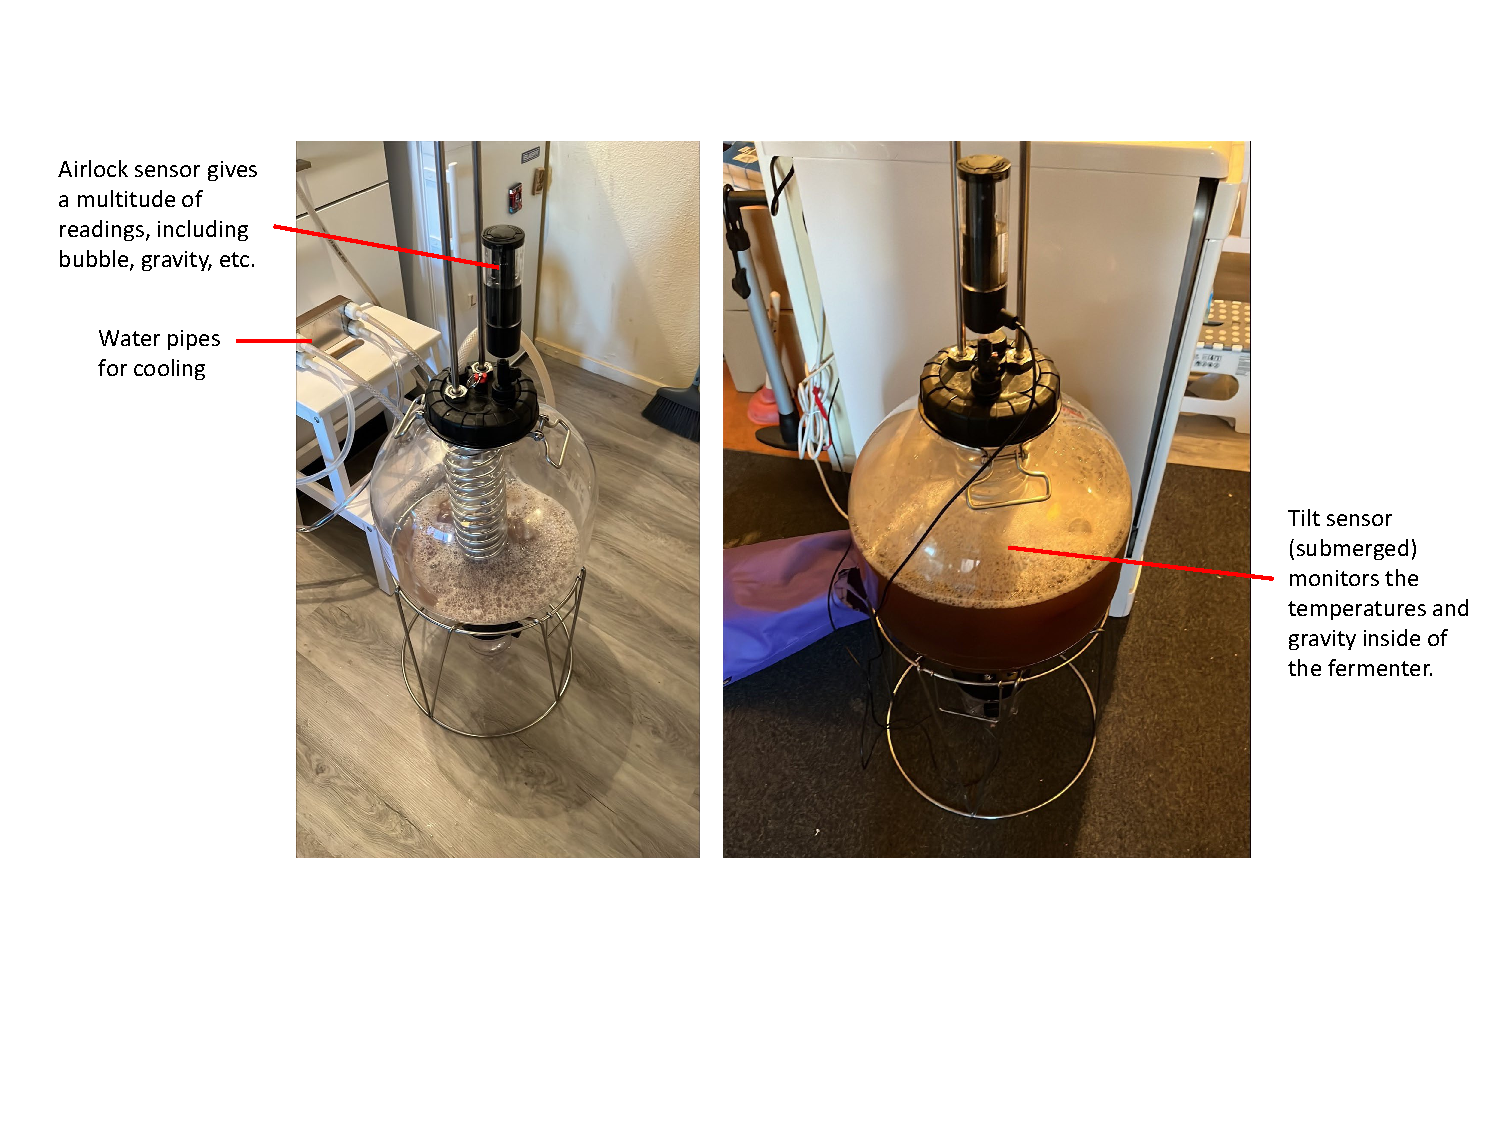
\includegraphics[scale=0.65]{figures/workbench_fermenter.pdf}
  \caption{The fermenter before (left) and after (right) being filled up with wort.}
  \label{fig:workbench_fermenter}
\end{figure}

\newpage
The other PEs that do not directly attach to the fermenter are installed in the same room, shown in Figure \ref{fig:workbench_other}. 

\begin{figure}[hbt!]
  \centering
  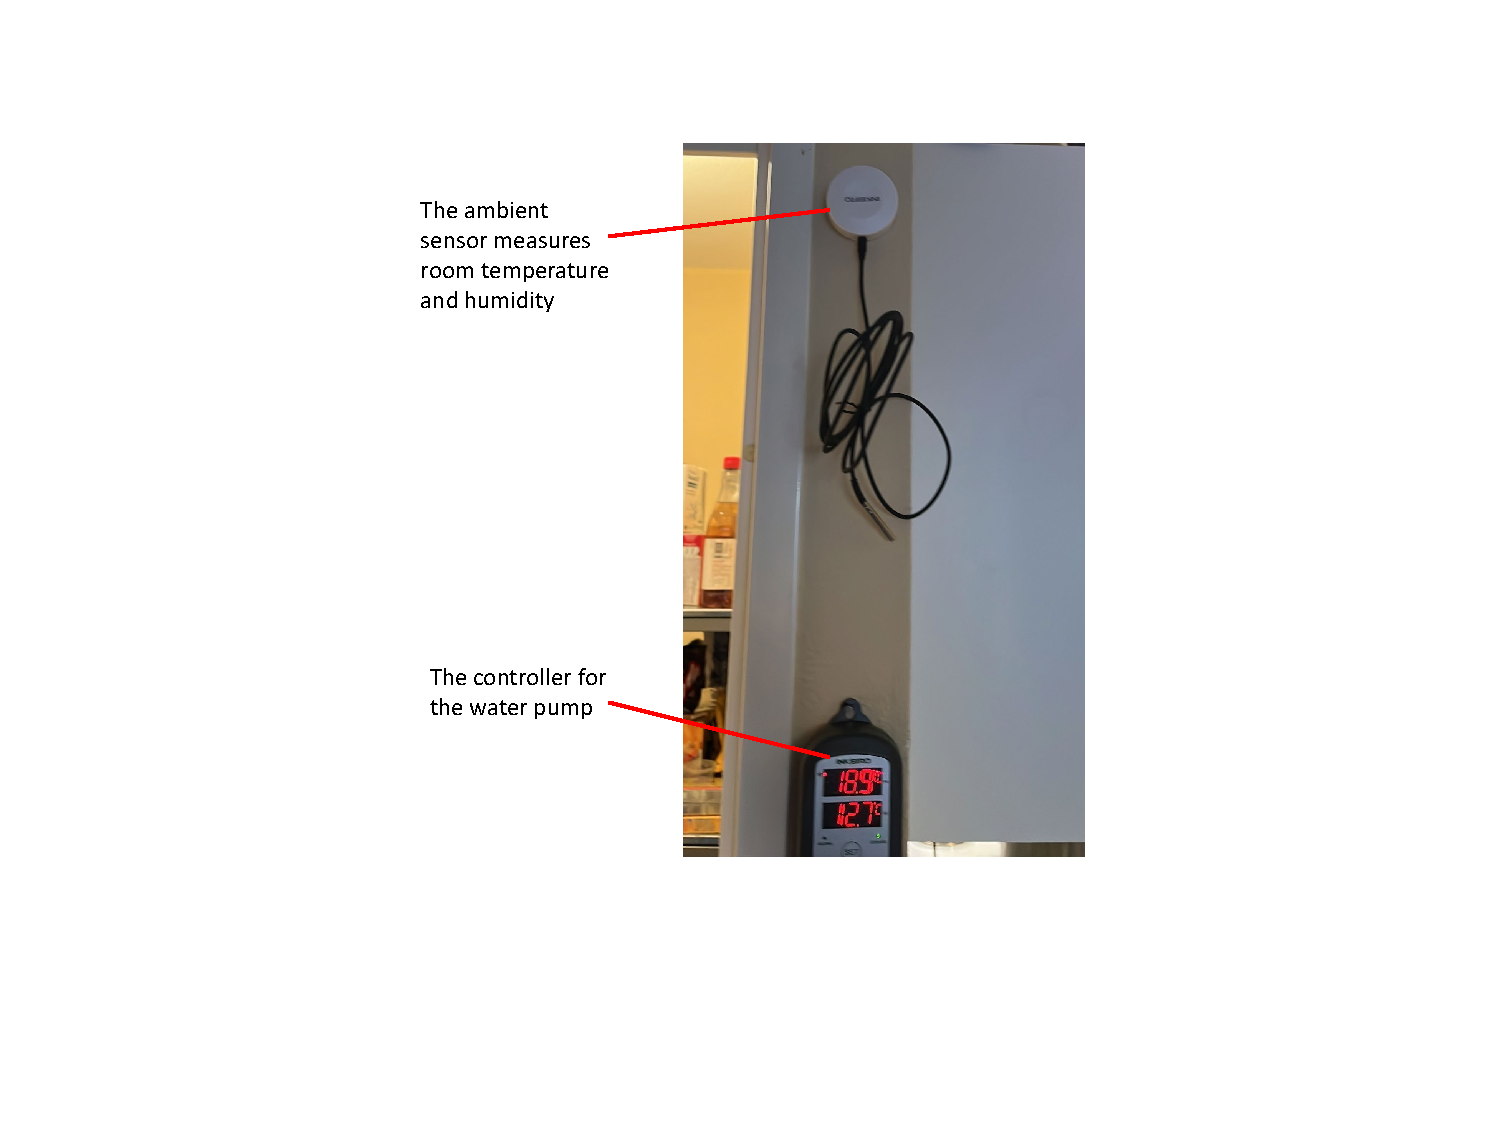
\includegraphics[scale=0.65]{figures/workbench_other.pdf}
  \caption{More devices at the workbench}
  \label{fig:workbench_other}
\end{figure}

Figure \ref{fig:workbench_map} shows the overall network topology of the workbench.

\begin{figure}[hbt!]
  \centering
  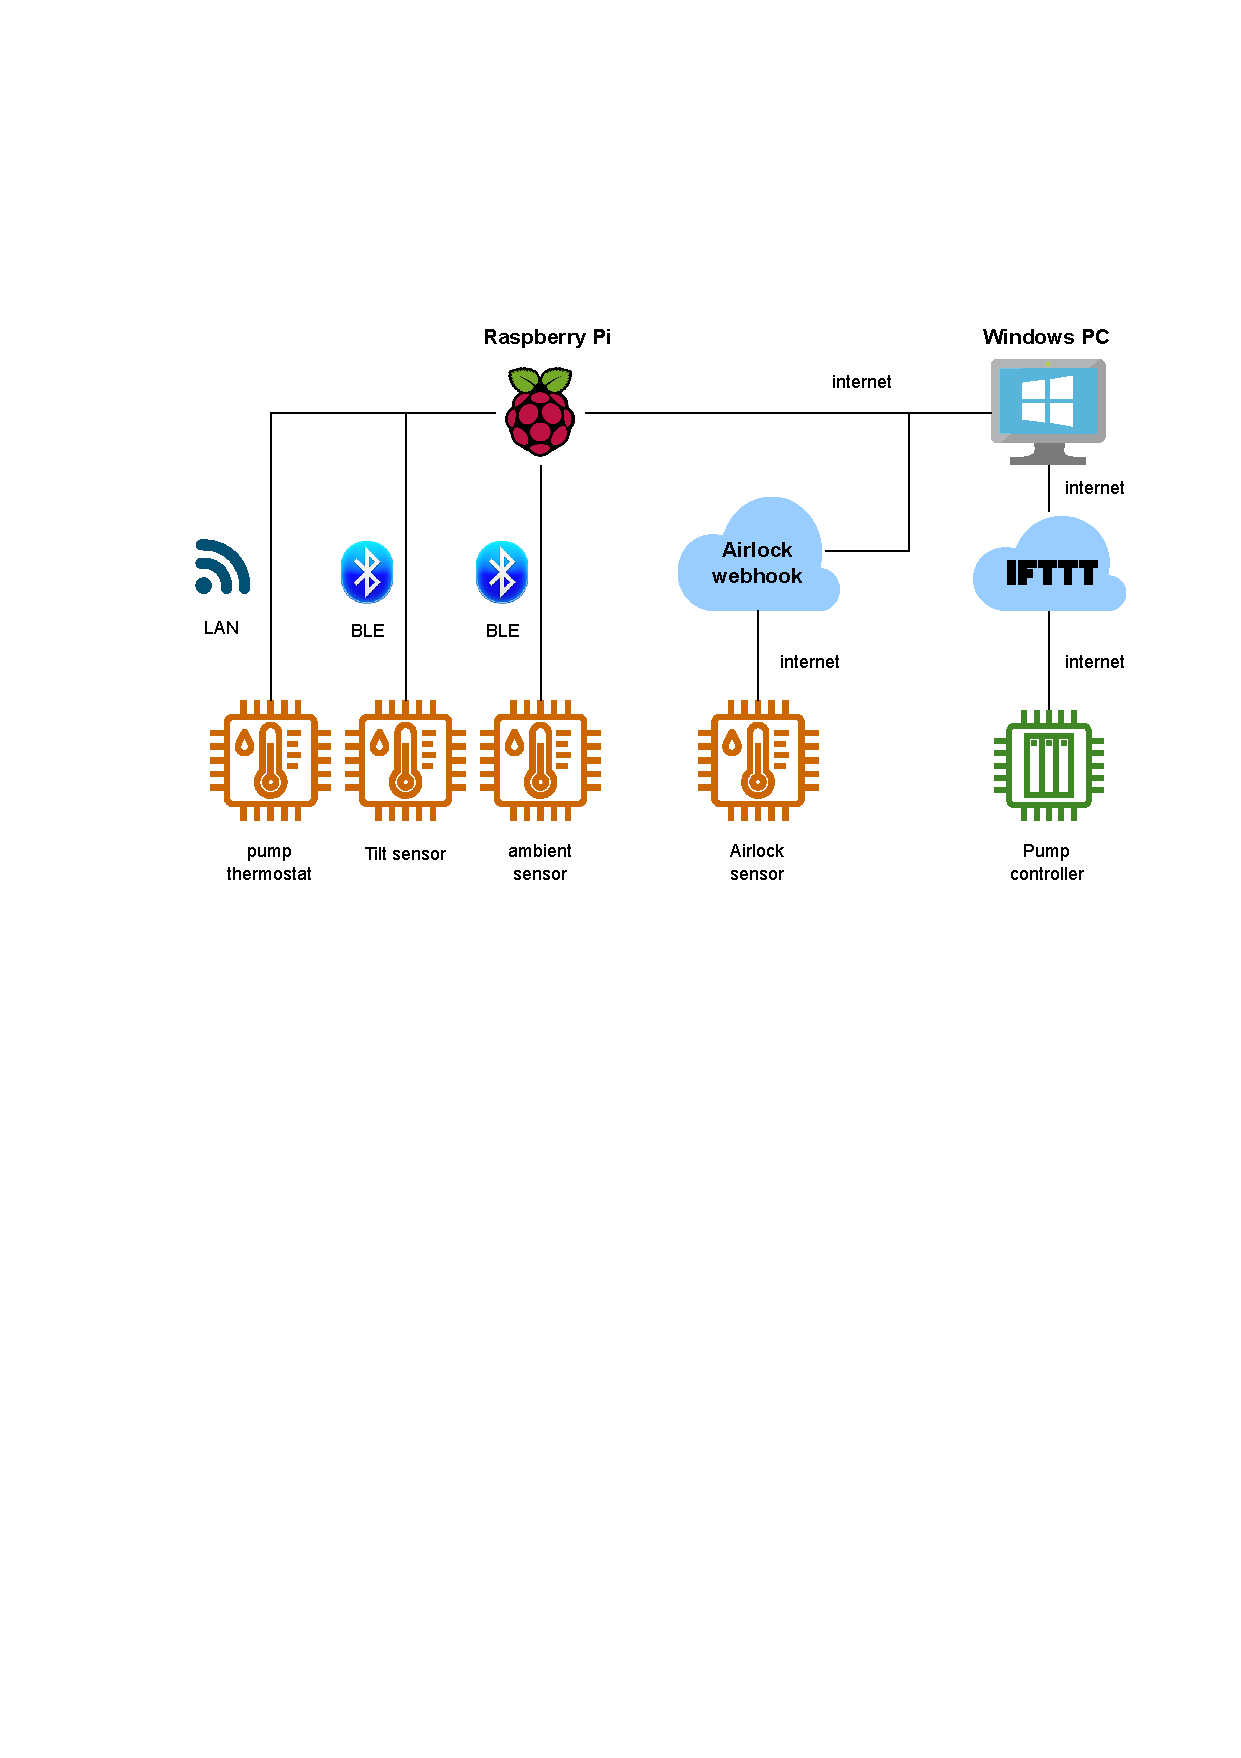
\includegraphics[scale=0.65]{figures/workbench_map.pdf}
  \caption[Network topology of the workbench]{Network topology of the workbench. Airlock sensor has an officially supported cloud server. The PC can send the control signals to the pump controller via IFTTT, which is a popular commercial service for home/smart phone automation.}
  \label{fig:workbench_map}
\end{figure}

\chapter{Kafka primer} \label{apd:kafka}
Kafka has been used extensively alongside our frameworks as a data management tool. This section will briefly introduce the main concepts of Kafka, and the advantages that make it suitable under DT contexts.

Kafka is considered an event streaming platform \cite{Kafka} that is based on the publish/subscribe design pattern (illustrated in Figure \ref{fig:kafka_example}). It supports three fundamental aspects:

\begin{figure}[hbt!]
  \centering
  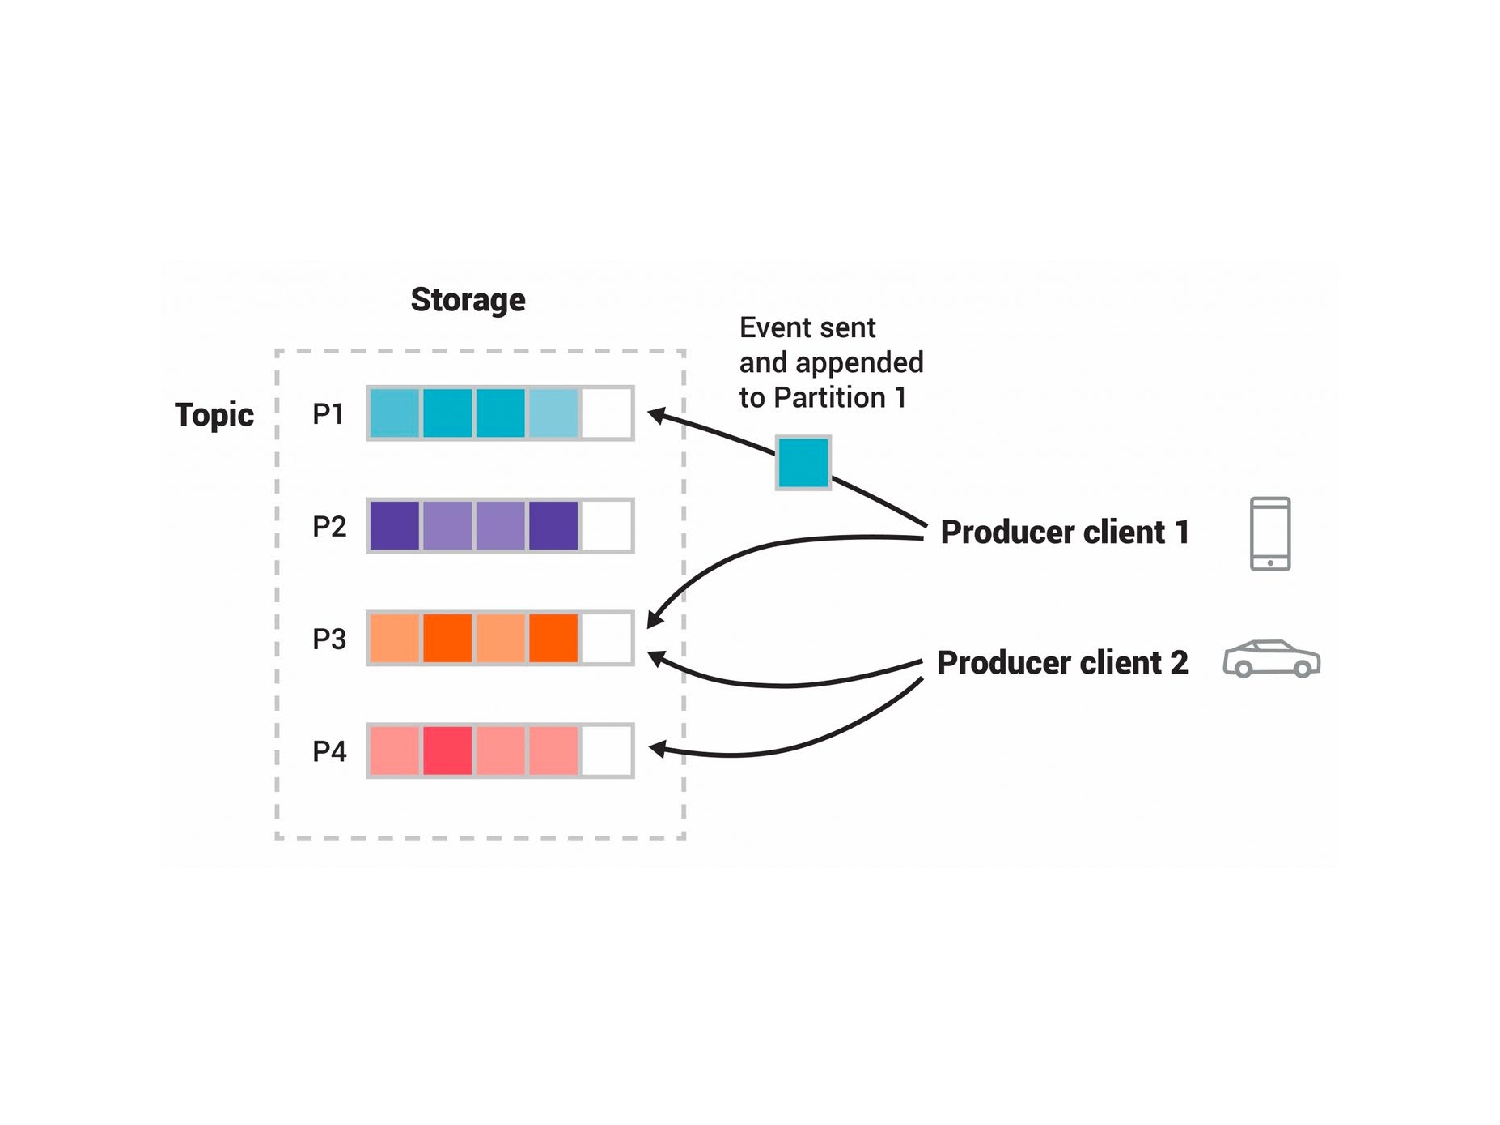
\includegraphics[scale=0.4]{figures/kafka_example.pdf}
  \caption [An example Kafka architecture] {An example Kafka architecture \cite{Kafka}}
  \label{fig:kafka_example}
\end{figure}

\begin{itemize}
\item \textbf{Publish} and \textbf{Subscribe}: the ``producer" publishes events which can be subscribed by the ``consumer". The event streams are maintained by the Kafka server such that the producer and consumer can be agnostic and decoupled to each other.
\item \textbf{Process}: referred to the enrichment and transformations of the event data. Processing can happen in real-time or in retrospect.
\item \textbf{Storage}: The event data can be stored for a duration chosen by the user.
\end{itemize} 

What makes Kafka stand out from alternative solutions of similar style (e.g., MQTT) is its emphasis on durable and persistent messages, which allows data manipulation being done either when the messages occur or retrospectively. This is important as DTs often deal with both real-time and historical data in a hybrid fashion. In Kafka the persistent storage can be accessed by ``offset tracking", a mechanism analogous to the pointer of a data structure. 

Another DT aspect Kafka manages to address is the compartmentalization of data semantics through ``topic" assignments. Conventional SQL-based approach depends on active query to data tables which sits passively in the binary objects. In contrast, Kafka turns the situation in which the data are proactively partitioned to distinct topics, while the users are ensured that different data compartments will be independent and readily accessible.  


\chapter{FMI revisit} \label{apd:fmi}
This section explains why the \texttt{FMUImporter} of Ptolemy II has failed to perform the FMUs in our case study. Our troubleshooting results indicate the root cause is due to the improper calling sequence of the FMI functions.

It begins with the FMUs used in the microbrewery DT having the property of nonlinear algebraic loop, that is, when the outputs and inputs of the model have mutual dependencies. According to the official FMI specification \cite{fmidoc}, it states that such algebraic loops may be solved in the \textit{Initialization Mode} by setting initial values to the involved inputs/outputs, which allows the solver to iteratively compute them to a convergence---when the interdependent input-output pair reaches an arbitrarily small difference. Listing \ref{lst:fmi} shows the pseudocode of what a valid calling sequence should look like.

\begin{lstlisting}[language=Python, label={lst:fmi}, caption={Resolving algebraic loop in the Initialization Mode}]
instantiate()
setupExperiment(startTime=startTime, stopTime=stopTime) 
enterInitializationMode()
setReal(inputs, values) # setting values to model variables
exitInitializationMode()
\end{lstlisting} 

However, the internal implementation of \texttt{FMUImporter} does not follow this strictly, as one can see in Figure \ref{fig:fmi_error}, in there the initialization function is terminated before setting the start values. Consequentially, the output value returns \texttt{NaN} since the FMU could not resolve the algebraic loop.

\begin{figure}[hbt!]
  \centering
  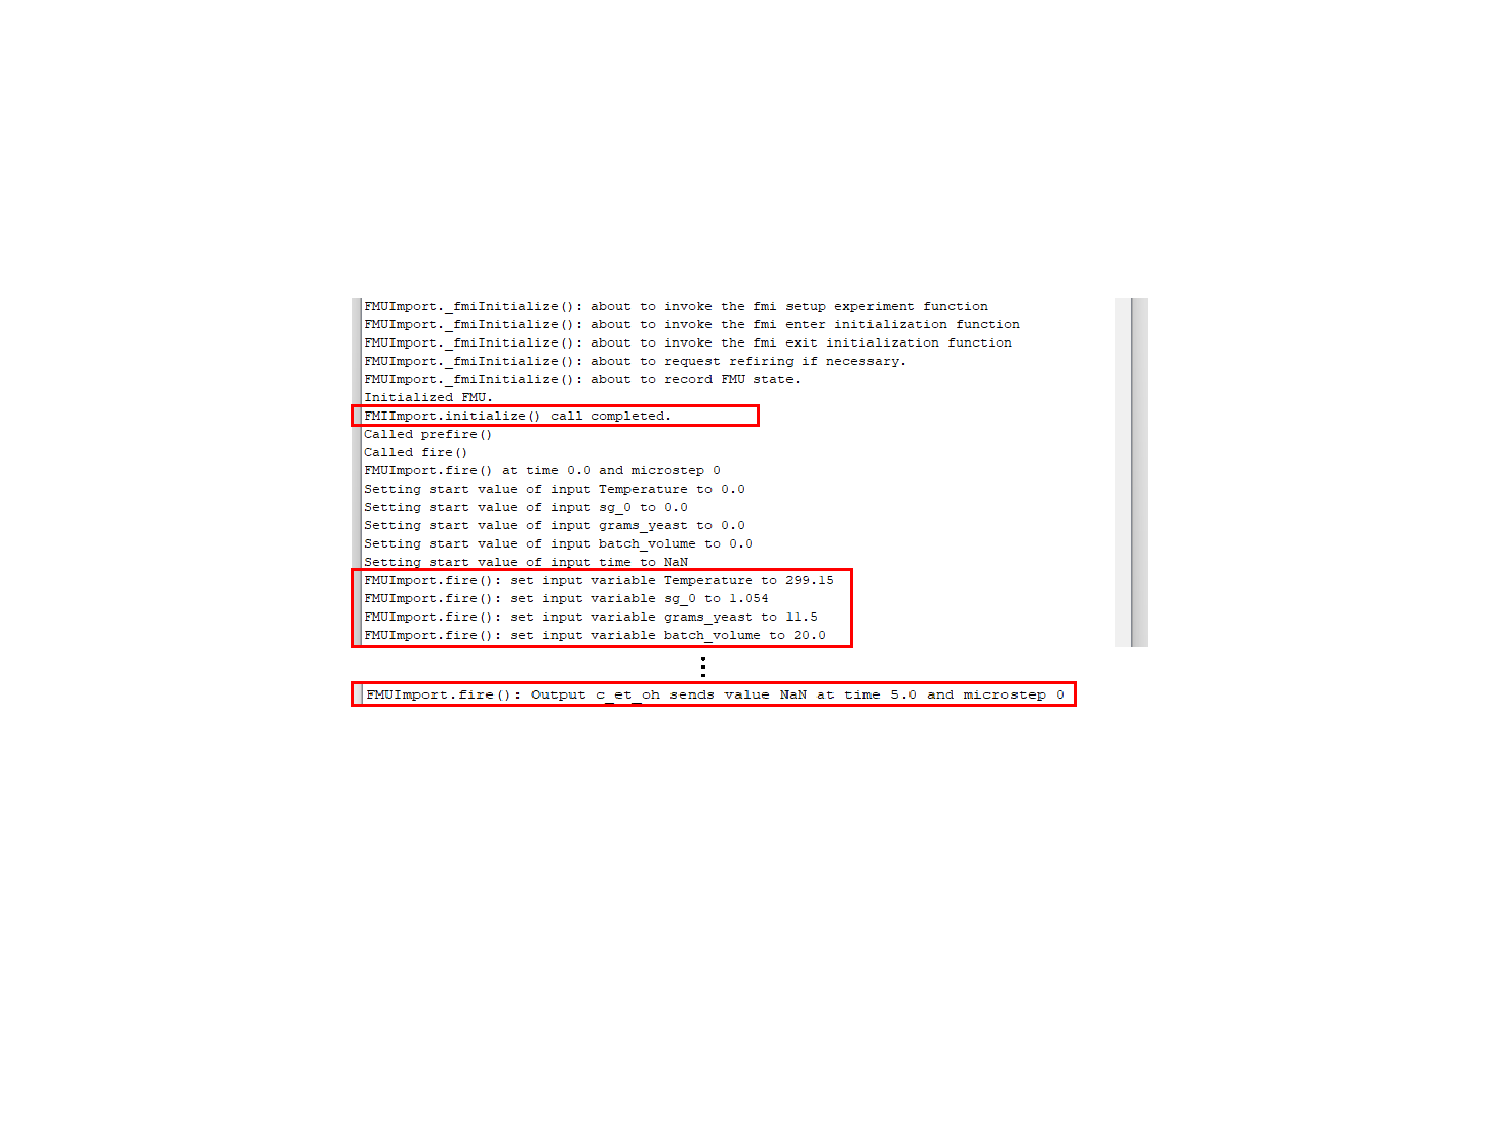
\includegraphics[scale=0.8]{figures/fmi_error.pdf}
  \caption {Incorrect function calling sequence by Ptolemy II}
  \label{fig:fmi_error}
\end{figure}

Due to this reason, along with several other limitations of Ptolemy II regarding its supports for FMI, we decide not to adopt the \texttt{FMUImporter} in the microbrewery DT implementation.

\chapter{Human-in-the-loop control scheme} \label{apd:humanloop}
This section dedicates to showcase the human-in-the-loop concept for S2---Production Control---of the microbrewery DT. For the context, a water pump is used regulate the fermentation temperature by circulating the water from a ice-cooled bucket to the fermenter and back, forming a closed water-cooling circuit. 

In the original S2, The models in VEs generate control signals that switch the power of the water pump in PEs. This operation is fully automated. Alternatively, in the human-in-the-loop version, the projection of water-cooling heat transfer is informed (via a client terminal as shown in Figure \ref{fig:hmi_client}) to the operator by the models, enabling the operator to make human judgments about replacing the ice in the bucket in order to alter the effect time of the temperature regulation. The two control schemes are illustrated Figure \ref{fig:hmi_scheme}.

\begin{figure}[hbt!]
  \centering
  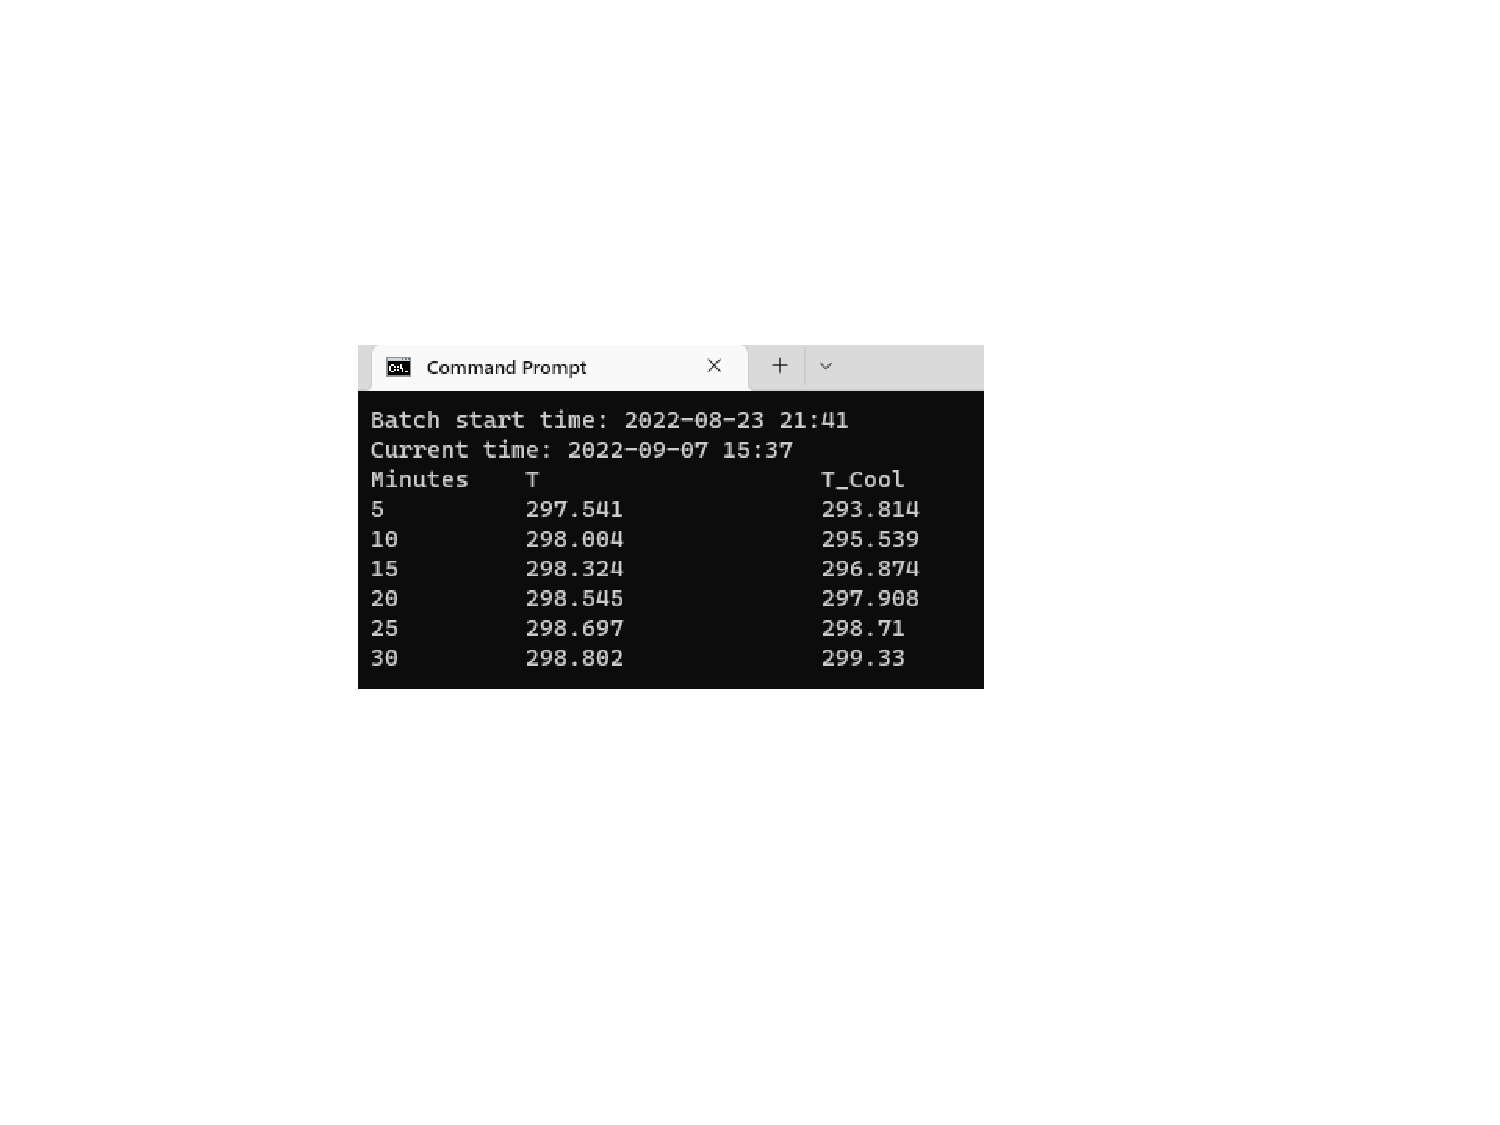
\includegraphics[scale=0.5]{figures/hmi_client.pdf}
  \caption [The client interface]{The client interface displaying a 30-minute heat predictions of the water-cooling setup}
  \label{fig:hmi_client}
\end{figure}

\begin{figure}[hbt!]
  \centering
  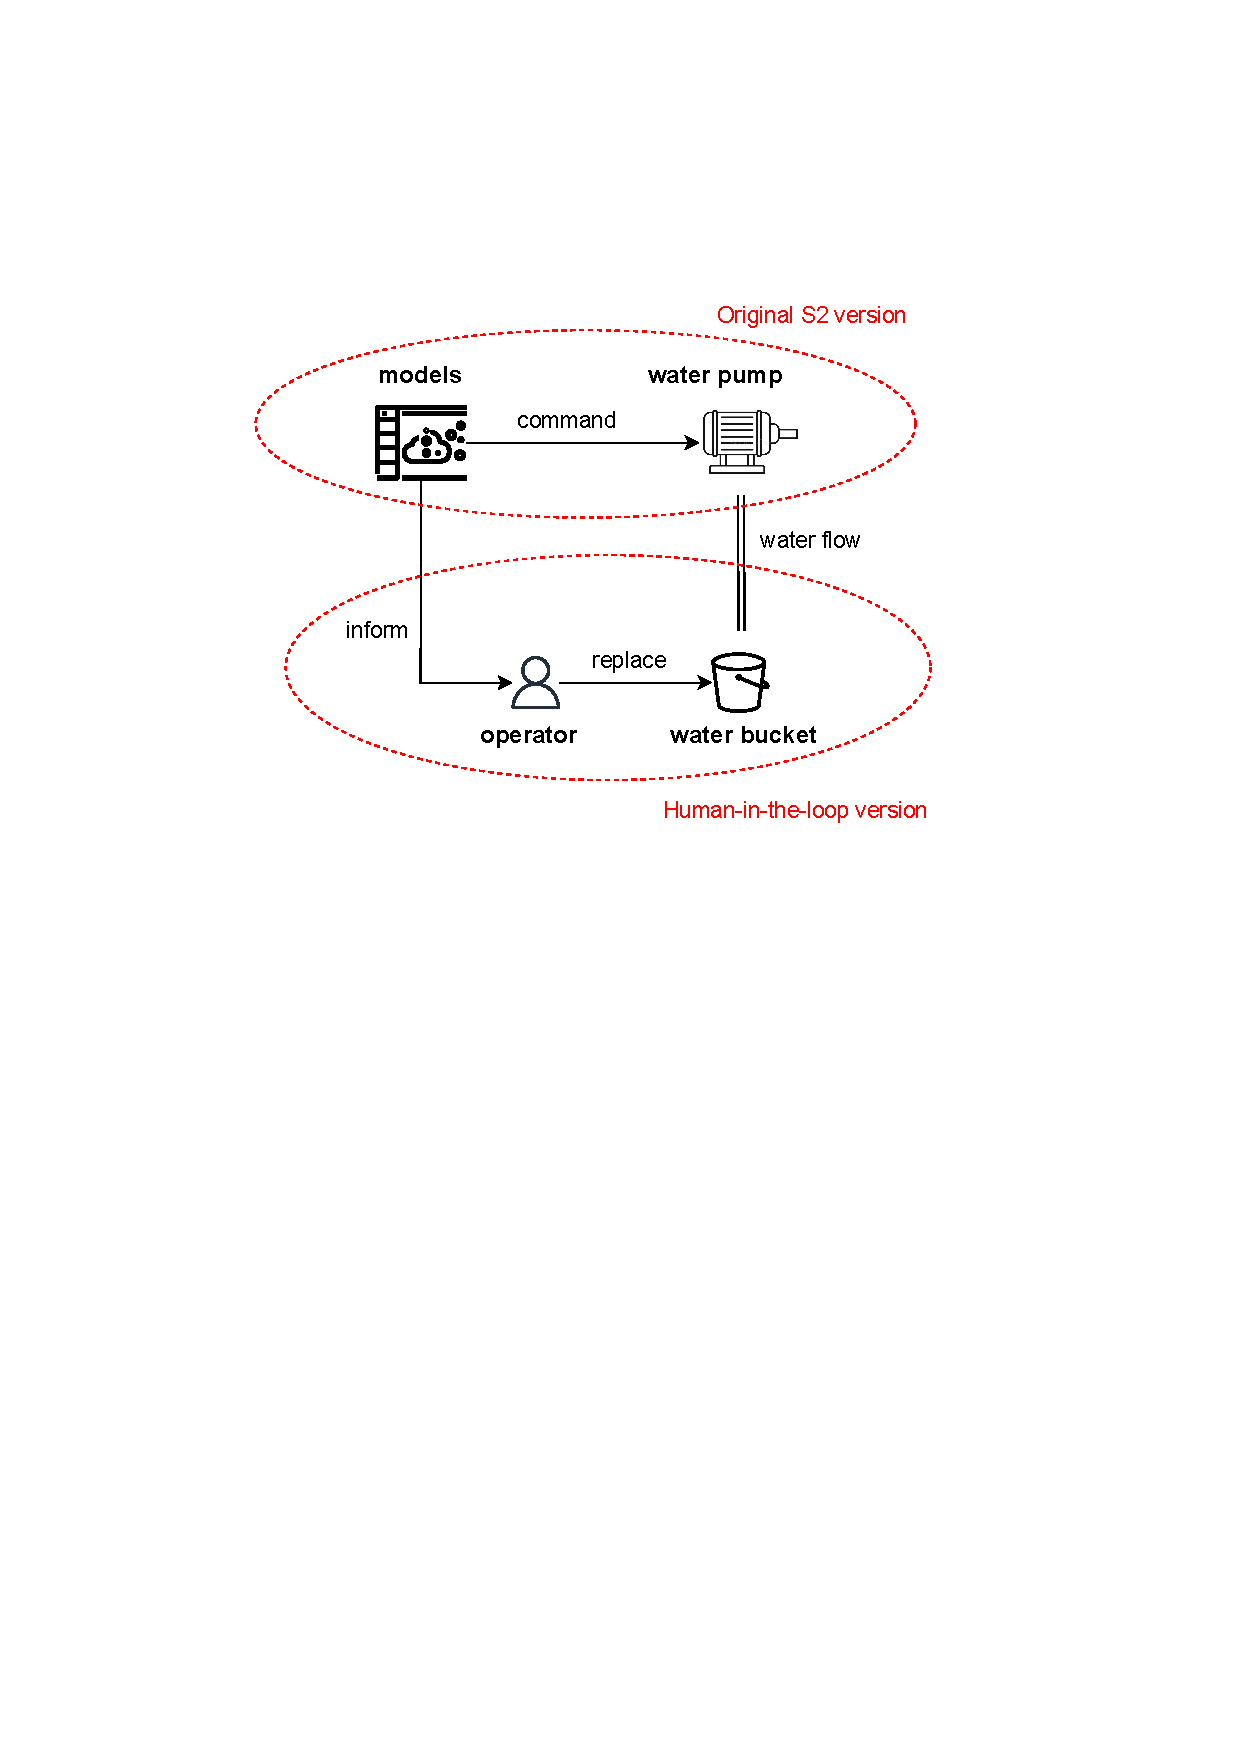
\includegraphics[scale=0.6]{figures/hmi_scheme.pdf}
  \caption {The original S2 (top) and the human-in-the-loop control scheme (bottom)}
  \label{fig:hmi_scheme}
\end{figure}

The real water circuit setup at the workbench is shown in Figure \ref{fig:workbench_bucket}.

\begin{figure}[hbt!]
  \centering
  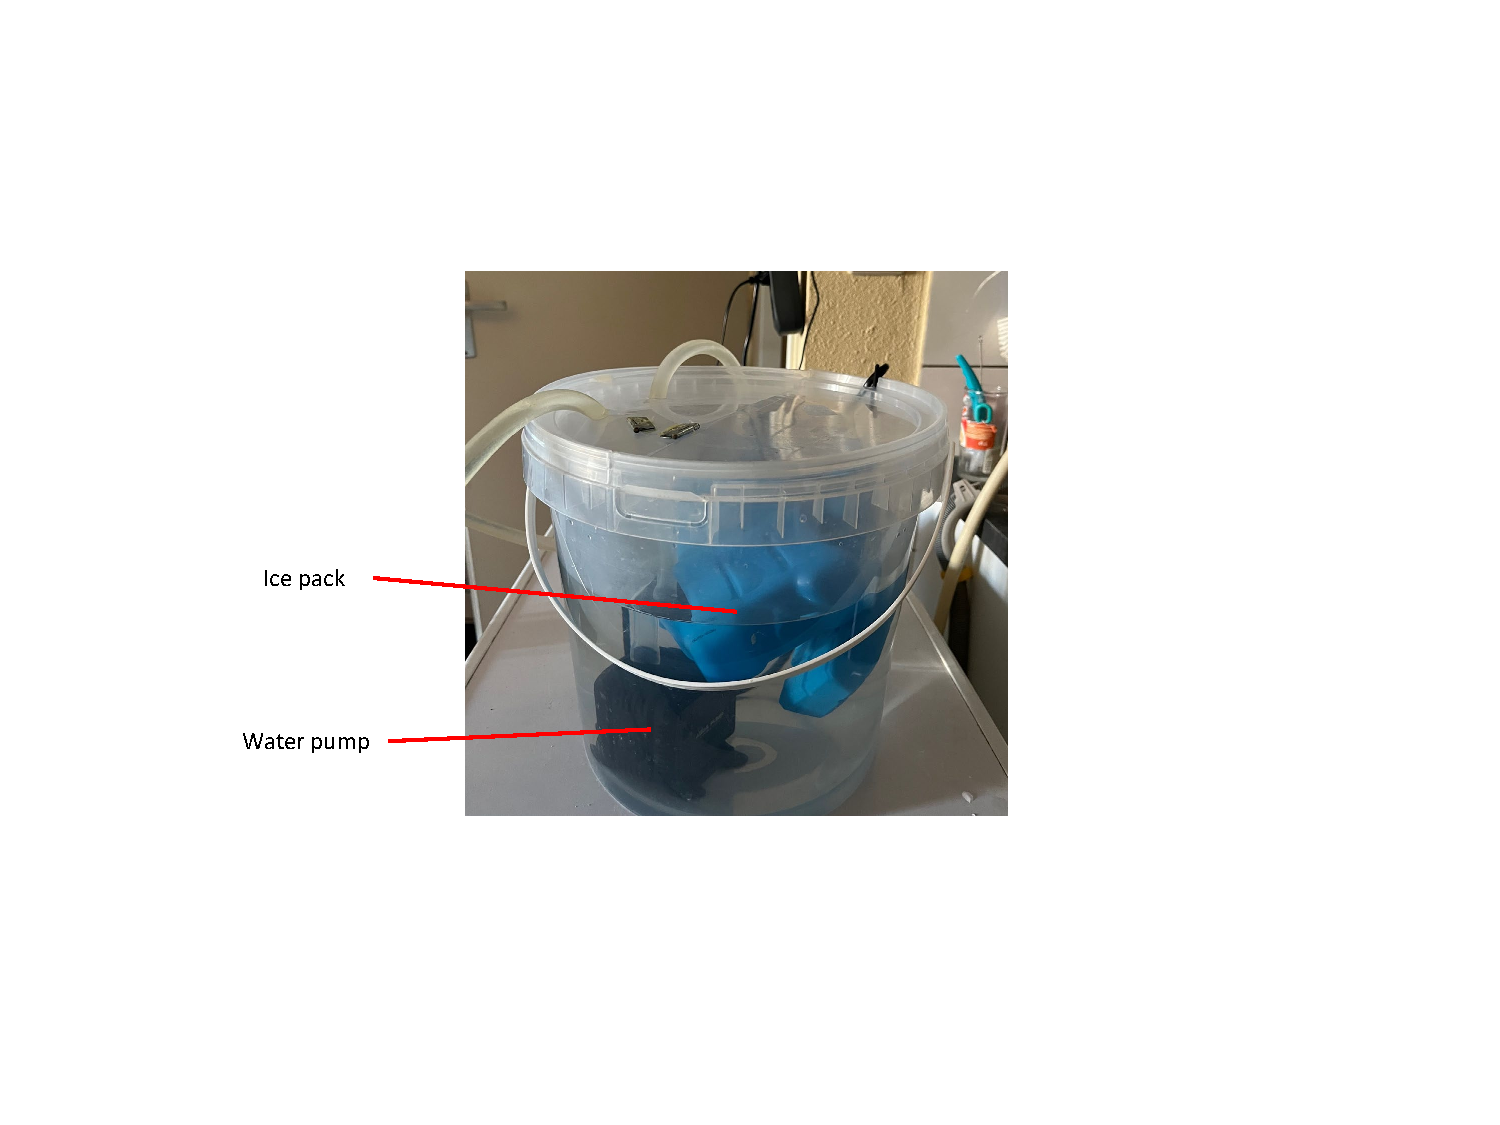
\includegraphics[scale=0.65]{figures/workbench_bucket.pdf}
  \caption{Water circuit setup}
  \label{fig:workbench_bucket}
\end{figure}

This demonstration describes a proof-of-concept for human-machine integration in a DT, although not being the primary research objective of this study, we recognize its importance for especially DTs in the bioprocessing domains.


\end{appendices}


\end{document}
